\documentclass[twoside]{book}

% Packages required by doxygen
\usepackage{calc}
\usepackage{doxygen}
\usepackage{graphicx}
\usepackage[utf8]{inputenc}
\usepackage{makeidx}
\usepackage{multicol}
\usepackage{multirow}
\usepackage{textcomp}
\usepackage[table]{xcolor}

% Font selection
\usepackage[T1]{fontenc}
\usepackage{mathptmx}
\usepackage[scaled=.90]{helvet}
\usepackage{courier}
\usepackage{amssymb}
\usepackage{sectsty}
\renewcommand{\familydefault}{\sfdefault}
\allsectionsfont{%
  \fontseries{bc}\selectfont%
  \color{darkgray}%
}
\renewcommand{\DoxyLabelFont}{%
  \fontseries{bc}\selectfont%
  \color{darkgray}%
}

% Page & text layout
\usepackage{geometry}
\geometry{%
  a4paper,%
  top=2.5cm,%
  bottom=2.5cm,%
  left=2.5cm,%
  right=2.5cm%
}
\tolerance=750
\hfuzz=15pt
\hbadness=750
\setlength{\emergencystretch}{15pt}
\setlength{\parindent}{0cm}
\setlength{\parskip}{0.2cm}
\makeatletter
\renewcommand{\paragraph}{%
  \@startsection{paragraph}{4}{0ex}{-1.0ex}{1.0ex}{%
    \normalfont\normalsize\bfseries\SS@parafont%
  }%
}
\renewcommand{\subparagraph}{%
  \@startsection{subparagraph}{5}{0ex}{-1.0ex}{1.0ex}{%
    \normalfont\normalsize\bfseries\SS@subparafont%
  }%
}
\makeatother

% Headers & footers
\usepackage{fancyhdr}
\pagestyle{fancyplain}
\fancyhead[LE]{\fancyplain{}{\bfseries\thepage}}
\fancyhead[CE]{\fancyplain{}{}}
\fancyhead[RE]{\fancyplain{}{\bfseries\leftmark}}
\fancyhead[LO]{\fancyplain{}{\bfseries\rightmark}}
\fancyhead[CO]{\fancyplain{}{}}
\fancyhead[RO]{\fancyplain{}{\bfseries\thepage}}
\fancyfoot[LE]{\fancyplain{}{}}
\fancyfoot[CE]{\fancyplain{}{}}
\fancyfoot[RE]{\fancyplain{}{\bfseries\scriptsize Generated on Mon Nov 30 2020 00\-:09\-:28 for Nysse\-Meni by Doxygen }}
\fancyfoot[LO]{\fancyplain{}{\bfseries\scriptsize Generated on Mon Nov 30 2020 00\-:09\-:28 for Nysse\-Meni by Doxygen }}
\fancyfoot[CO]{\fancyplain{}{}}
\fancyfoot[RO]{\fancyplain{}{}}
\renewcommand{\footrulewidth}{0.4pt}
\renewcommand{\chaptermark}[1]{%
  \markboth{#1}{}%
}
\renewcommand{\sectionmark}[1]{%
  \markright{\thesection\ #1}%
}

% Indices & bibliography
\usepackage{natbib}
\usepackage[titles]{tocloft}
\setcounter{tocdepth}{3}
\setcounter{secnumdepth}{5}
\makeindex

% Hyperlinks (required, but should be loaded last)
\usepackage{ifpdf}
\ifpdf
  \usepackage[pdftex,pagebackref=true]{hyperref}
\else
  \usepackage[ps2pdf,pagebackref=true]{hyperref}
\fi
\hypersetup{%
  colorlinks=true,%
  linkcolor=blue,%
  citecolor=blue,%
  unicode%
}

% Custom commands
\newcommand{\clearemptydoublepage}{%
  \newpage{\pagestyle{empty}\cleardoublepage}%
}


%===== C O N T E N T S =====

\begin{document}

% Titlepage & ToC
\hypersetup{pageanchor=false}
\pagenumbering{roman}
\begin{titlepage}
\vspace*{7cm}
\begin{center}%
{\Large Nysse\-Meni }\\
\vspace*{1cm}
{\large Generated by Doxygen 1.8.5}\\
\vspace*{0.5cm}
{\small Mon Nov 30 2020 00:09:28}\\
\end{center}
\end{titlepage}
\clearemptydoublepage
\tableofcontents
\clearemptydoublepage
\pagenumbering{arabic}
\hypersetup{pageanchor=true}

%--- Begin generated contents ---
\chapter{Namespace Index}
\section{Namespace List}
Here is a list of all namespaces with brief descriptions\-:\begin{DoxyCompactList}
\item\contentsline{section}{\hyperlink{namespace_student_side}{Student\-Side} \\*Namespace Studen\-Side, Students own imlplementations to project }{\pageref{namespace_student_side}}{}
\item\contentsline{section}{\hyperlink{namespace_ui}{Ui} \\*Namespace \hyperlink{namespace_ui}{Ui} for dialog window class }{\pageref{namespace_ui}}{}
\end{DoxyCompactList}

\chapter{Hierarchical Index}
\section{Class Hierarchy}
This inheritance list is sorted roughly, but not completely, alphabetically\-:\begin{DoxyCompactList}
\item I\-Actor\begin{DoxyCompactList}
\item \contentsline{section}{Student\-Side\-:\-:Actor}{\pageref{class_student_side_1_1_actor}}{}
\end{DoxyCompactList}
\item I\-City\begin{DoxyCompactList}
\item \contentsline{section}{Student\-Side\-:\-:City}{\pageref{class_student_side_1_1_city}}{}
\end{DoxyCompactList}
\item I\-Statistics\begin{DoxyCompactList}
\item \contentsline{section}{Student\-Side\-:\-:Statistics}{\pageref{class_student_side_1_1_statistics}}{}
\end{DoxyCompactList}
\item I\-Vehicle\begin{DoxyCompactList}
\item \contentsline{section}{Student\-Side\-:\-:Vehicle}{\pageref{class_student_side_1_1_vehicle}}{}
\end{DoxyCompactList}
\item Q\-Dialog\begin{DoxyCompactList}
\item \contentsline{section}{Student\-Side\-:\-:Dialog\-Game\-Settings}{\pageref{class_student_side_1_1_dialog_game_settings}}{}
\end{DoxyCompactList}
\item Q\-Graphics\-Pixmap\-Item\begin{DoxyCompactList}
\item \contentsline{section}{Student\-Side\-:\-:Actor\-Item}{\pageref{class_student_side_1_1_actor_item}}{}
\item \contentsline{section}{Student\-Side\-:\-:Nuke\-Actor}{\pageref{class_student_side_1_1_nuke_actor}}{}
\item \contentsline{section}{Student\-Side\-:\-:player\-Actor}{\pageref{class_student_side_1_1player_actor}}{}
\end{DoxyCompactList}
\item Q\-Main\-Window\begin{DoxyCompactList}
\item \contentsline{section}{Student\-Side\-:\-:Mainwindow}{\pageref{class_student_side_1_1_mainwindow}}{}
\end{DoxyCompactList}
\item Q\-Object\begin{DoxyCompactList}
\item \contentsline{section}{Student\-Side\-:\-:Game\-Engine}{\pageref{class_student_side_1_1_game_engine}}{}
\end{DoxyCompactList}
\item \contentsline{section}{qt\-\_\-meta\-\_\-stringdata\-\_\-\-Student\-Side\-\_\-\-\_\-\-Dialog\-Game\-Settings\-\_\-t}{\pageref{structqt__meta__stringdata___student_side_____dialog_game_settings__t}}{}
\item \contentsline{section}{qt\-\_\-meta\-\_\-stringdata\-\_\-\-Student\-Side\-\_\-\-\_\-\-Game\-Engine\-\_\-t}{\pageref{structqt__meta__stringdata___student_side_____game_engine__t}}{}
\item \contentsline{section}{qt\-\_\-meta\-\_\-stringdata\-\_\-\-Student\-Side\-\_\-\-\_\-\-Mainwindow\-\_\-t}{\pageref{structqt__meta__stringdata___student_side_____mainwindow__t}}{}
\item \contentsline{section}{Ui\-\_\-\-Dialog\-Game\-Settings}{\pageref{class_ui___dialog_game_settings}}{}
\begin{DoxyCompactList}
\item \contentsline{section}{Ui\-:\-:Dialog\-Game\-Settings}{\pageref{class_ui_1_1_dialog_game_settings}}{}
\end{DoxyCompactList}
\item \contentsline{section}{Ui\-\_\-\-Main\-Window}{\pageref{class_ui___main_window}}{}
\begin{DoxyCompactList}
\item \contentsline{section}{Ui\-:\-:Main\-Window}{\pageref{class_ui_1_1_main_window}}{}
\end{DoxyCompactList}
\end{DoxyCompactList}

\chapter{Class Index}
\section{Class List}
Here are the classes, structs, unions and interfaces with brief descriptions\-:\begin{DoxyCompactList}
\item\contentsline{section}{\hyperlink{class_student_side_1_1_actor}{Student\-Side\-::\-Actor} }{\pageref{class_student_side_1_1_actor}}{}
\item\contentsline{section}{\hyperlink{class_student_side_1_1_actor_item}{Student\-Side\-::\-Actor\-Item} }{\pageref{class_student_side_1_1_actor_item}}{}
\item\contentsline{section}{\hyperlink{class_student_side_1_1_city}{Student\-Side\-::\-City} \\*That defines city operations }{\pageref{class_student_side_1_1_city}}{}
\item\contentsline{section}{\hyperlink{class_student_side_1_1_dialog_game_settings}{Student\-Side\-::\-Dialog\-Game\-Settings} \\*The Dialog\-Gane\-Settings class sets up dialog window to get pre settings for the main game }{\pageref{class_student_side_1_1_dialog_game_settings}}{}
\item\contentsline{section}{\hyperlink{class_student_side_1_1_game_engine}{Student\-Side\-::\-Game\-Engine} \\*The Init\-Game\-Engine class is for setting the game up. It launches dialog window for settings and initializes gamewindow }{\pageref{class_student_side_1_1_game_engine}}{}
\item\contentsline{section}{\hyperlink{class_student_side_1_1_mainwindow}{Student\-Side\-::\-Mainwindow} \\*The mainwindow class }{\pageref{class_student_side_1_1_mainwindow}}{}
\item\contentsline{section}{\hyperlink{class_student_side_1_1_nuke_actor}{Student\-Side\-::\-Nuke\-Actor} }{\pageref{class_student_side_1_1_nuke_actor}}{}
\item\contentsline{section}{\hyperlink{class_student_side_1_1player_actor}{Student\-Side\-::player\-Actor} }{\pageref{class_student_side_1_1player_actor}}{}
\item\contentsline{section}{\hyperlink{class_student_side_1_1_statistics}{Student\-Side\-::\-Statistics} }{\pageref{class_student_side_1_1_statistics}}{}
\item\contentsline{section}{\hyperlink{class_student_side_1_1_vehicle}{Student\-Side\-::\-Vehicle} }{\pageref{class_student_side_1_1_vehicle}}{}
\end{DoxyCompactList}

\chapter{File Index}
\section{File List}
Here is a list of all files with brief descriptions\-:\begin{DoxyCompactList}
\item\contentsline{section}{\hyperlink{actor_8cpp}{actor.\-cpp} }{\pageref{actor_8cpp}}{}
\item\contentsline{section}{\hyperlink{actor_8hh}{actor.\-hh} \\*The Actor class }{\pageref{actor_8hh}}{}
\item\contentsline{section}{\hyperlink{actoritem_8cpp}{actoritem.\-cpp} }{\pageref{actoritem_8cpp}}{}
\item\contentsline{section}{\hyperlink{actoritem_8hh}{actoritem.\-hh} \\*The Actor\-Item class }{\pageref{actoritem_8hh}}{}
\item\contentsline{section}{\hyperlink{city_8cpp}{city.\-cpp} }{\pageref{city_8cpp}}{}
\item\contentsline{section}{\hyperlink{city_8hh}{city.\-hh} \\*Defines city operations for game that has been inherited from i\-City }{\pageref{city_8hh}}{}
\item\contentsline{section}{\hyperlink{creategame_8cpp}{creategame.\-cpp} }{\pageref{creategame_8cpp}}{}
\item\contentsline{section}{\hyperlink{dialoggamesettings_8cpp}{dialoggamesettings.\-cpp} }{\pageref{dialoggamesettings_8cpp}}{}
\item\contentsline{section}{\hyperlink{dialoggamesettings_8hh}{dialoggamesettings.\-hh} }{\pageref{dialoggamesettings_8hh}}{}
\item\contentsline{section}{\hyperlink{gameengine_8cpp}{gameengine.\-cpp} }{\pageref{gameengine_8cpp}}{}
\item\contentsline{section}{\hyperlink{gameengine_8hh}{gameengine.\-hh} }{\pageref{gameengine_8hh}}{}
\item\contentsline{section}{\hyperlink{main_8cc}{main.\-cc} }{\pageref{main_8cc}}{}
\item\contentsline{section}{\hyperlink{mainwindow_8cpp}{mainwindow.\-cpp} }{\pageref{mainwindow_8cpp}}{}
\item\contentsline{section}{\hyperlink{mainwindow_8hh}{mainwindow.\-hh} }{\pageref{mainwindow_8hh}}{}
\item\contentsline{section}{\hyperlink{nukeactor_8cpp}{nukeactor.\-cpp} }{\pageref{nukeactor_8cpp}}{}
\item\contentsline{section}{\hyperlink{nukeactor_8hh}{nukeactor.\-hh} }{\pageref{nukeactor_8hh}}{}
\item\contentsline{section}{\hyperlink{playeractor_8cpp}{playeractor.\-cpp} }{\pageref{playeractor_8cpp}}{}
\item\contentsline{section}{\hyperlink{playeractor_8hh}{playeractor.\-hh} \\*The player\-Actor class }{\pageref{playeractor_8hh}}{}
\item\contentsline{section}{\hyperlink{statistics_8cpp}{statistics.\-cpp} }{\pageref{statistics_8cpp}}{}
\item\contentsline{section}{\hyperlink{statistics_8hh}{statistics.\-hh} }{\pageref{statistics_8hh}}{}
\item\contentsline{section}{\hyperlink{vehicle_8cpp}{vehicle.\-cpp} }{\pageref{vehicle_8cpp}}{}
\item\contentsline{section}{\hyperlink{vehicle_8hh}{vehicle.\-hh} \\*The Vehicle class }{\pageref{vehicle_8hh}}{}
\end{DoxyCompactList}

\chapter{Namespace Documentation}
\hypertarget{namespace_student_side}{\section{Student\-Side Namespace Reference}
\label{namespace_student_side}\index{Student\-Side@{Student\-Side}}
}


namespace Studen\-Side, Students own imlplementations to project  


\subsection*{Classes}
\begin{DoxyCompactItemize}
\item 
class \hyperlink{class_student_side_1_1_actor}{Actor}
\item 
class \hyperlink{class_student_side_1_1_actor_item}{Actor\-Item}
\item 
class \hyperlink{class_student_side_1_1_city}{City}
\item 
class \hyperlink{class_student_side_1_1_dialog_game_settings}{Dialog\-Game\-Settings}
\begin{DoxyCompactList}\small\item\em The Dialog\-Gane\-Settings class sets up dialog window to get pre settings for the main game. \end{DoxyCompactList}\item 
class \hyperlink{class_student_side_1_1_game_engine}{Game\-Engine}
\begin{DoxyCompactList}\small\item\em The Init\-Game\-Engine class is for setting the game up. It launches dialog window for settings and initializes gamewindow. \end{DoxyCompactList}\item 
class \hyperlink{class_student_side_1_1_mainwindow}{Mainwindow}
\begin{DoxyCompactList}\small\item\em The mainwindow class. \end{DoxyCompactList}\item 
class \hyperlink{class_student_side_1_1_nuke_actor}{Nuke\-Actor}
\begin{DoxyCompactList}\small\item\em The \hyperlink{class_student_side_1_1_nuke_actor}{Nuke\-Actor} class. \end{DoxyCompactList}\item 
class \hyperlink{class_student_side_1_1player_actor}{player\-Actor}
\item 
class \hyperlink{class_student_side_1_1_statistics}{Statistics}
\item 
class \hyperlink{class_student_side_1_1_vehicle}{Vehicle}
\end{DoxyCompactItemize}


\subsection{Detailed Description}
namespace Studen\-Side, Students own imlplementations to project 
\hypertarget{namespace_ui}{\section{Ui Namespace Reference}
\label{namespace_ui}\index{Ui@{Ui}}
}


namespace \hyperlink{namespace_ui}{Ui} for dialog window class  


\subsection*{Classes}
\begin{DoxyCompactItemize}
\item 
class \hyperlink{class_ui_1_1_dialog_game_settings}{Dialog\-Game\-Settings}
\item 
class \hyperlink{class_ui_1_1_main_window}{Main\-Window}
\end{DoxyCompactItemize}


\subsection{Detailed Description}
namespace \hyperlink{namespace_ui}{Ui} for dialog window class \hyperlink{namespace_ui}{Ui} namespace for mainwindow class. 
\chapter{Class Documentation}
\hypertarget{class_student_side_1_1_actor}{\section{Student\-Side\-:\-:Actor Class Reference}
\label{class_student_side_1_1_actor}\index{Student\-Side\-::\-Actor@{Student\-Side\-::\-Actor}}
}


{\ttfamily \#include $<$actor.\-hh$>$}

Inheritance diagram for Student\-Side\-:\-:Actor\-:\begin{figure}[H]
\begin{center}
\leavevmode
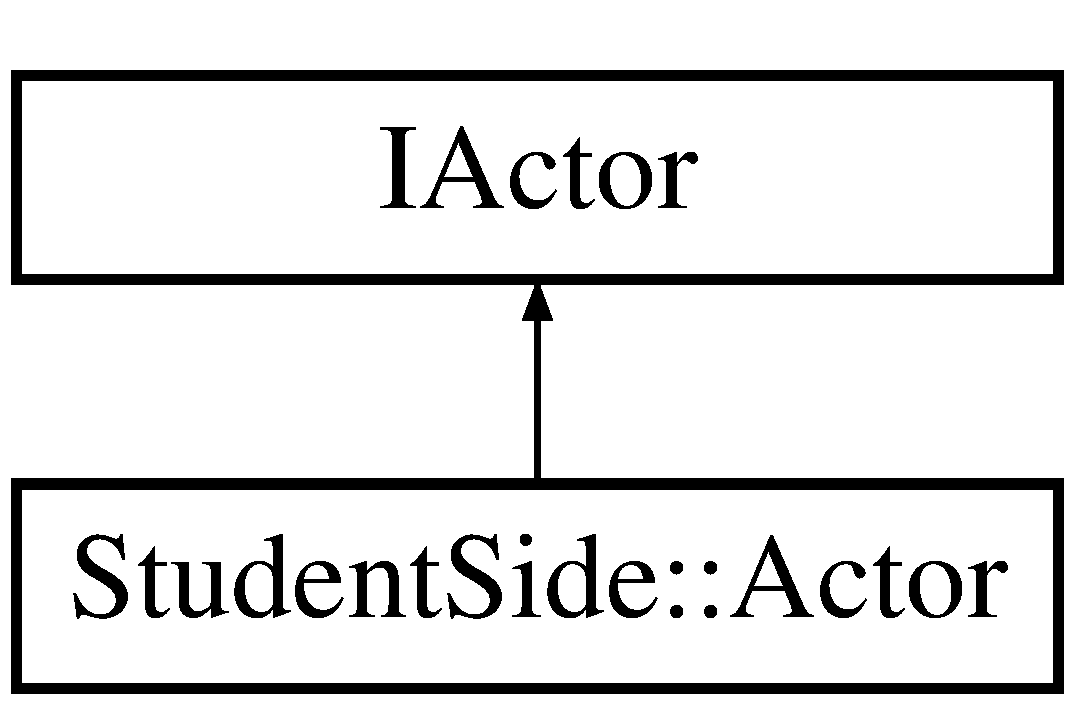
\includegraphics[height=2.000000cm]{class_student_side_1_1_actor}
\end{center}
\end{figure}
\subsection*{Public Member Functions}
\begin{DoxyCompactItemize}
\item 
\hyperlink{class_student_side_1_1_actor_a975c8c762266aaa7a77bd66fc4ec52f8}{Actor} ()
\begin{DoxyCompactList}\small\item\em Constructor for Actors. \end{DoxyCompactList}\item 
\hyperlink{class_student_side_1_1_actor_ae5f1f32ef2603cff6d9f91648ad723df}{$\sim$\-Actor} ()
\begin{DoxyCompactList}\small\item\em Destructor. \end{DoxyCompactList}\item 
Interface\-::\-Location \hyperlink{class_student_side_1_1_actor_a7da7be8bf80fd2cb6ecccb5643c5550b}{give\-Location} () const override
\begin{DoxyCompactList}\small\item\em give\-Location method gives location from Interface \end{DoxyCompactList}\item 
void \hyperlink{class_student_side_1_1_actor_ac3027790dbf5d48a783931a39876b16f}{move} (Interface\-::\-Location loc) override
\begin{DoxyCompactList}\small\item\em move the actor to wanted location \end{DoxyCompactList}\item 
bool \hyperlink{class_student_side_1_1_actor_ae43895e750efd94a11ed0377de1541a2}{is\-Removed} () const override
\begin{DoxyCompactList}\small\item\em is\-Removed checks if actor has been removed \end{DoxyCompactList}\item 
void \hyperlink{class_student_side_1_1_actor_ac5be31d931bf28cfd9044c991ea7ad18}{remove} () override
\begin{DoxyCompactList}\small\item\em remove actor \end{DoxyCompactList}\item 
void \hyperlink{class_student_side_1_1_actor_a9e2ebb8ad1118556222cb153e9a4cd3e}{add\-Location} (Interface\-::\-Location $\ast$location)
\begin{DoxyCompactList}\small\item\em add\-Location to actor \end{DoxyCompactList}\end{DoxyCompactItemize}


\subsection{Constructor \& Destructor Documentation}
\hypertarget{class_student_side_1_1_actor_a975c8c762266aaa7a77bd66fc4ec52f8}{\index{Student\-Side\-::\-Actor@{Student\-Side\-::\-Actor}!Actor@{Actor}}
\index{Actor@{Actor}!StudentSide::Actor@{Student\-Side\-::\-Actor}}
\subsubsection[{Actor}]{\setlength{\rightskip}{0pt plus 5cm}Student\-Side\-::\-Actor\-::\-Actor (
\begin{DoxyParamCaption}
{}
\end{DoxyParamCaption}
)}}\label{class_student_side_1_1_actor_a975c8c762266aaa7a77bd66fc4ec52f8}


Constructor for Actors. 

\begin{DoxyPrecond}{Precondition}
-\/ 
\end{DoxyPrecond}
\hypertarget{class_student_side_1_1_actor_ae5f1f32ef2603cff6d9f91648ad723df}{\index{Student\-Side\-::\-Actor@{Student\-Side\-::\-Actor}!$\sim$\-Actor@{$\sim$\-Actor}}
\index{$\sim$\-Actor@{$\sim$\-Actor}!StudentSide::Actor@{Student\-Side\-::\-Actor}}
\subsubsection[{$\sim$\-Actor}]{\setlength{\rightskip}{0pt plus 5cm}Student\-Side\-::\-Actor\-::$\sim$\-Actor (
\begin{DoxyParamCaption}
{}
\end{DoxyParamCaption}
)}}\label{class_student_side_1_1_actor_ae5f1f32ef2603cff6d9f91648ad723df}


Destructor. 

\begin{DoxyPrecond}{Precondition}
-\/ 
\end{DoxyPrecond}


\subsection{Member Function Documentation}
\hypertarget{class_student_side_1_1_actor_a9e2ebb8ad1118556222cb153e9a4cd3e}{\index{Student\-Side\-::\-Actor@{Student\-Side\-::\-Actor}!add\-Location@{add\-Location}}
\index{add\-Location@{add\-Location}!StudentSide::Actor@{Student\-Side\-::\-Actor}}
\subsubsection[{add\-Location}]{\setlength{\rightskip}{0pt plus 5cm}void Student\-Side\-::\-Actor\-::add\-Location (
\begin{DoxyParamCaption}
\item[{Interface\-::\-Location $\ast$}]{location}
\end{DoxyParamCaption}
)}}\label{class_student_side_1_1_actor_a9e2ebb8ad1118556222cb153e9a4cd3e}


add\-Location to actor 


\begin{DoxyParams}{Parameters}
{\em location} & of a actor \\
\hline
\end{DoxyParams}
\begin{DoxyPrecond}{Precondition}
-\/ 
\end{DoxyPrecond}
\begin{DoxyPostcond}{Postcondition}
Exception guarantee\-: Minimum 
\end{DoxyPostcond}
\hypertarget{class_student_side_1_1_actor_a7da7be8bf80fd2cb6ecccb5643c5550b}{\index{Student\-Side\-::\-Actor@{Student\-Side\-::\-Actor}!give\-Location@{give\-Location}}
\index{give\-Location@{give\-Location}!StudentSide::Actor@{Student\-Side\-::\-Actor}}
\subsubsection[{give\-Location}]{\setlength{\rightskip}{0pt plus 5cm}Interface\-::\-Location Student\-Side\-::\-Actor\-::give\-Location (
\begin{DoxyParamCaption}
{}
\end{DoxyParamCaption}
) const\hspace{0.3cm}{\ttfamily [override]}}}\label{class_student_side_1_1_actor_a7da7be8bf80fd2cb6ecccb5643c5550b}


give\-Location method gives location from Interface 

\begin{DoxyPrecond}{Precondition}
-\/ 
\end{DoxyPrecond}
\begin{DoxyPostcond}{Postcondition}
Exception guarantee\-: Strong 
\end{DoxyPostcond}
\begin{DoxyReturn}{Returns}
location of actor 
\end{DoxyReturn}
\hypertarget{class_student_side_1_1_actor_ae43895e750efd94a11ed0377de1541a2}{\index{Student\-Side\-::\-Actor@{Student\-Side\-::\-Actor}!is\-Removed@{is\-Removed}}
\index{is\-Removed@{is\-Removed}!StudentSide::Actor@{Student\-Side\-::\-Actor}}
\subsubsection[{is\-Removed}]{\setlength{\rightskip}{0pt plus 5cm}bool Student\-Side\-::\-Actor\-::is\-Removed (
\begin{DoxyParamCaption}
{}
\end{DoxyParamCaption}
) const\hspace{0.3cm}{\ttfamily [override]}}}\label{class_student_side_1_1_actor_ae43895e750efd94a11ed0377de1541a2}


is\-Removed checks if actor has been removed 

\begin{DoxyReturn}{Returns}
boolean value of if actor is removed 
\end{DoxyReturn}
\begin{DoxyPrecond}{Precondition}
-\/ 
\end{DoxyPrecond}
\begin{DoxyPostcond}{Postcondition}
Exception guarantee\-: Basic 
\end{DoxyPostcond}
\hypertarget{class_student_side_1_1_actor_ac3027790dbf5d48a783931a39876b16f}{\index{Student\-Side\-::\-Actor@{Student\-Side\-::\-Actor}!move@{move}}
\index{move@{move}!StudentSide::Actor@{Student\-Side\-::\-Actor}}
\subsubsection[{move}]{\setlength{\rightskip}{0pt plus 5cm}void Student\-Side\-::\-Actor\-::move (
\begin{DoxyParamCaption}
\item[{Interface\-::\-Location}]{loc}
\end{DoxyParamCaption}
)\hspace{0.3cm}{\ttfamily [override]}}}\label{class_student_side_1_1_actor_ac3027790dbf5d48a783931a39876b16f}


move the actor to wanted location 


\begin{DoxyParams}{Parameters}
{\em loc,location} & of the actor \\
\hline
\end{DoxyParams}
\begin{DoxyPrecond}{Precondition}
loc.\-x $>$ 0, loc.\-y $>$ 0, loc.\-x $<$ 1100, loc.\-y $<$ 590 
\end{DoxyPrecond}
\begin{DoxyPostcond}{Postcondition}
Exception guarantee\-: Strong 
\end{DoxyPostcond}
\hypertarget{class_student_side_1_1_actor_ac5be31d931bf28cfd9044c991ea7ad18}{\index{Student\-Side\-::\-Actor@{Student\-Side\-::\-Actor}!remove@{remove}}
\index{remove@{remove}!StudentSide::Actor@{Student\-Side\-::\-Actor}}
\subsubsection[{remove}]{\setlength{\rightskip}{0pt plus 5cm}void Student\-Side\-::\-Actor\-::remove (
\begin{DoxyParamCaption}
{}
\end{DoxyParamCaption}
)\hspace{0.3cm}{\ttfamily [override]}}}\label{class_student_side_1_1_actor_ac5be31d931bf28cfd9044c991ea7ad18}


remove actor 

\begin{DoxyPrecond}{Precondition}
-\/ 
\end{DoxyPrecond}
\begin{DoxyPostcond}{Postcondition}
Exception guarantee\-: nothrow 
\end{DoxyPostcond}


The documentation for this class was generated from the following files\-:\begin{DoxyCompactItemize}
\item 
Game/\hyperlink{actor_8hh}{actor.\-hh}\item 
Game/\hyperlink{actor_8cpp}{actor.\-cpp}\end{DoxyCompactItemize}

\hypertarget{class_student_side_1_1_actor_item}{\section{Student\-Side\-:\-:Actor\-Item Class Reference}
\label{class_student_side_1_1_actor_item}\index{Student\-Side\-::\-Actor\-Item@{Student\-Side\-::\-Actor\-Item}}
}


{\ttfamily \#include $<$actoritem.\-hh$>$}

Inheritance diagram for Student\-Side\-:\-:Actor\-Item\-:\begin{figure}[H]
\begin{center}
\leavevmode
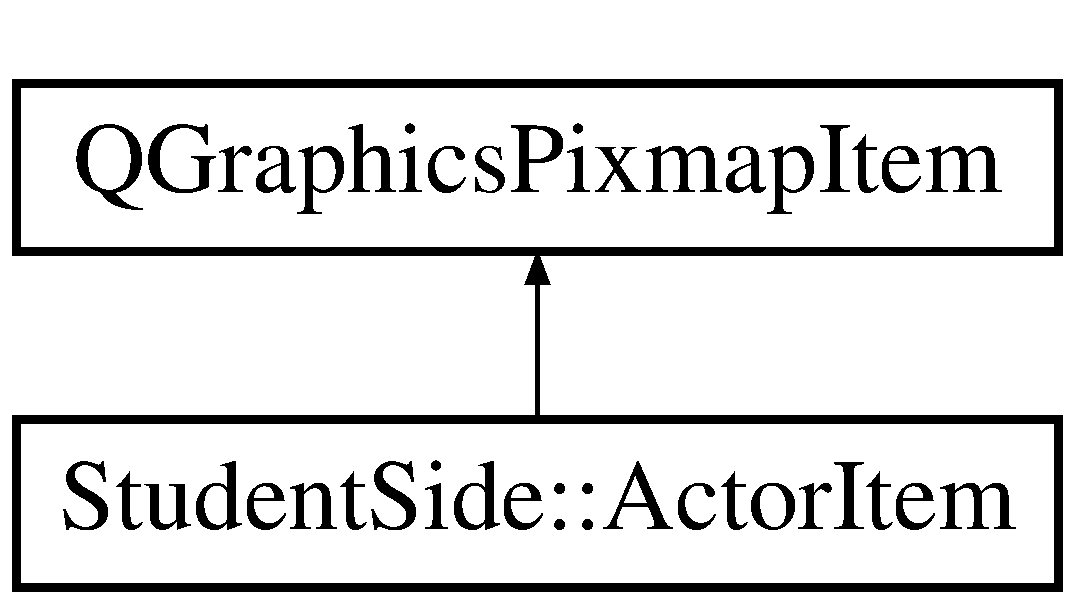
\includegraphics[height=2.000000cm]{class_student_side_1_1_actor_item}
\end{center}
\end{figure}
\subsection*{Public Member Functions}
\begin{DoxyCompactItemize}
\item 
\hyperlink{class_student_side_1_1_actor_item_a741d8a8d3413683146380fa1311e7ffa}{Actor\-Item} (int \hyperlink{jquery_8js_a4c3eadaa5164016d2c340d495fc6e55e}{x}, int y, int type=0)
\begin{DoxyCompactList}\small\item\em \hyperlink{class_student_side_1_1_actor_item}{Actor\-Item} constructor that sets the pictures for actors. \end{DoxyCompactList}\item 
\hyperlink{class_student_side_1_1_actor_item_a089e14fc439cd834bd8aec50cd55be87}{$\sim$\-Actor\-Item} ()
\begin{DoxyCompactList}\small\item\em Destructor. \end{DoxyCompactList}\item 
void \hyperlink{class_student_side_1_1_actor_item_a5a2f0d7ad57b6a71f24112682e46c9a3}{set\-Coord} (int \hyperlink{jquery_8js_a4c3eadaa5164016d2c340d495fc6e55e}{x}, int y)
\begin{DoxyCompactList}\small\item\em set\-Coord sets the actor\-Items position to the gameboard \end{DoxyCompactList}\end{DoxyCompactItemize}


\subsection{Constructor \& Destructor Documentation}
\hypertarget{class_student_side_1_1_actor_item_a741d8a8d3413683146380fa1311e7ffa}{\index{Student\-Side\-::\-Actor\-Item@{Student\-Side\-::\-Actor\-Item}!Actor\-Item@{Actor\-Item}}
\index{Actor\-Item@{Actor\-Item}!StudentSide::ActorItem@{Student\-Side\-::\-Actor\-Item}}
\subsubsection[{Actor\-Item}]{\setlength{\rightskip}{0pt plus 5cm}Student\-Side\-::\-Actor\-Item\-::\-Actor\-Item (
\begin{DoxyParamCaption}
\item[{int}]{x, }
\item[{int}]{y, }
\item[{int}]{type = {\ttfamily 0}}
\end{DoxyParamCaption}
)}}\label{class_student_side_1_1_actor_item_a741d8a8d3413683146380fa1311e7ffa}


\hyperlink{class_student_side_1_1_actor_item}{Actor\-Item} constructor that sets the pictures for actors. 


\begin{DoxyParams}{Parameters}
{\em x} & x-\/coordinate \\
\hline
{\em y} & y-\/coordinate \\
\hline
{\em type} & actor type \\
\hline
\end{DoxyParams}
\begin{DoxyPrecond}{Precondition}
coordinates must be in range of map coordinates. 
\end{DoxyPrecond}
\begin{DoxyPostcond}{Postcondition}
Exception guaranteed\-: nothrow 
\end{DoxyPostcond}
\hypertarget{class_student_side_1_1_actor_item_a089e14fc439cd834bd8aec50cd55be87}{\index{Student\-Side\-::\-Actor\-Item@{Student\-Side\-::\-Actor\-Item}!$\sim$\-Actor\-Item@{$\sim$\-Actor\-Item}}
\index{$\sim$\-Actor\-Item@{$\sim$\-Actor\-Item}!StudentSide::ActorItem@{Student\-Side\-::\-Actor\-Item}}
\subsubsection[{$\sim$\-Actor\-Item}]{\setlength{\rightskip}{0pt plus 5cm}Student\-Side\-::\-Actor\-Item\-::$\sim$\-Actor\-Item (
\begin{DoxyParamCaption}
{}
\end{DoxyParamCaption}
)}}\label{class_student_side_1_1_actor_item_a089e14fc439cd834bd8aec50cd55be87}


Destructor. 

\begin{DoxyPostcond}{Postcondition}
Exception guaranteed\-: nothrow 
\end{DoxyPostcond}


\subsection{Member Function Documentation}
\hypertarget{class_student_side_1_1_actor_item_a5a2f0d7ad57b6a71f24112682e46c9a3}{\index{Student\-Side\-::\-Actor\-Item@{Student\-Side\-::\-Actor\-Item}!set\-Coord@{set\-Coord}}
\index{set\-Coord@{set\-Coord}!StudentSide::ActorItem@{Student\-Side\-::\-Actor\-Item}}
\subsubsection[{set\-Coord}]{\setlength{\rightskip}{0pt plus 5cm}void Student\-Side\-::\-Actor\-Item\-::set\-Coord (
\begin{DoxyParamCaption}
\item[{int}]{x, }
\item[{int}]{y}
\end{DoxyParamCaption}
)}}\label{class_student_side_1_1_actor_item_a5a2f0d7ad57b6a71f24112682e46c9a3}


set\-Coord sets the actor\-Items position to the gameboard 


\begin{DoxyParams}{Parameters}
{\em x} & x-\/coordination \\
\hline
{\em y} & y-\/coordination \\
\hline
\end{DoxyParams}
\begin{DoxyPrecond}{Precondition}
-\/ 
\end{DoxyPrecond}
\begin{DoxyPostcond}{Postcondition}
Exception guaranteed\-: minimum 
\end{DoxyPostcond}


The documentation for this class was generated from the following files\-:\begin{DoxyCompactItemize}
\item 
Game/\hyperlink{actoritem_8hh}{actoritem.\-hh}\item 
Game/\hyperlink{actoritem_8cpp}{actoritem.\-cpp}\end{DoxyCompactItemize}

\hypertarget{class_student_side_1_1_city}{\section{Student\-Side\-:\-:City Class Reference}
\label{class_student_side_1_1_city}\index{Student\-Side\-::\-City@{Student\-Side\-::\-City}}
}


The \hyperlink{class_student_side_1_1_city}{City} class that defines city operations.  




{\ttfamily \#include $<$city.\-hh$>$}

Inheritance diagram for Student\-Side\-:\-:City\-:\begin{figure}[H]
\begin{center}
\leavevmode
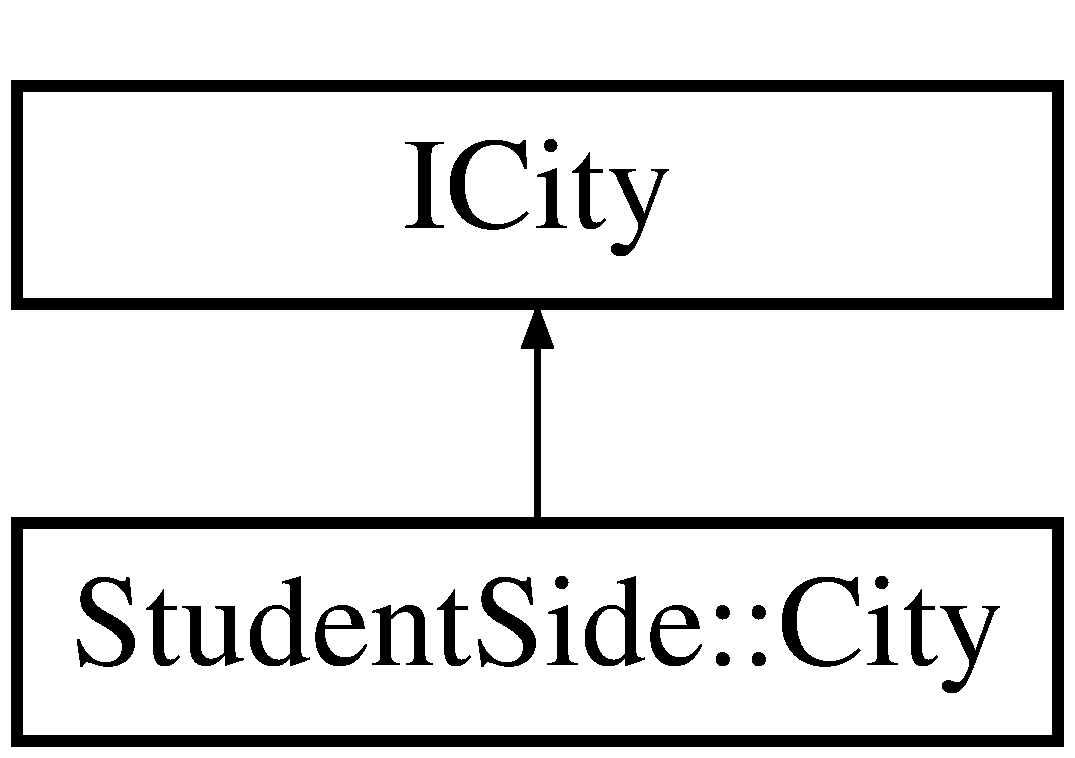
\includegraphics[height=2.000000cm]{class_student_side_1_1_city}
\end{center}
\end{figure}
\subsection*{Public Member Functions}
\begin{DoxyCompactItemize}
\item 
\hyperlink{class_student_side_1_1_city_ad5a0fd2a6e60fbd54bf0dfef0d5f849a}{City} ()
\begin{DoxyCompactList}\small\item\em \hyperlink{class_student_side_1_1_city}{City} constructor. \end{DoxyCompactList}\item 
\hyperlink{class_student_side_1_1_city_a9e98110785506a88ac9847755459988d}{$\sim$\-City} ()
\begin{DoxyCompactList}\small\item\em Destructor. \end{DoxyCompactList}\item 
void \hyperlink{class_student_side_1_1_city_a04accbc4ff8e507bc9b8cedae2444183}{set\-Background} (Q\-Image \&basicbackground, Q\-Image \&bigbackground) override
\begin{DoxyCompactList}\small\item\em set\-Background sets the map picture to game board. \end{DoxyCompactList}\item 
void \hyperlink{class_student_side_1_1_city_a7f57965f914ed8f3c544ce1324ba4fe8}{set\-Clock} (Q\-Time clock) override
\begin{DoxyCompactList}\small\item\em set\-Clock sets the time of a game clock. \end{DoxyCompactList}\item 
void \hyperlink{class_student_side_1_1_city_a54f4d302402630182a705d902c8e346a}{add\-Stop} (std\-::shared\-\_\-ptr$<$ Interface\-::\-I\-Stop $>$ stop) override
\begin{DoxyCompactList}\small\item\em add\-Stop adds a stop to the city. \end{DoxyCompactList}\item 
void \hyperlink{class_student_side_1_1_city_a10c22f1803f70837638d1f5543eb9627}{start\-Game} () override
\begin{DoxyCompactList}\small\item\em start\-Game changes game state to gamestate from initstate. \end{DoxyCompactList}\item 
void \hyperlink{class_student_side_1_1_city_af3c2bc7c60238c935c42b66e6f8d257a}{add\-Actor} (std\-::shared\-\_\-ptr$<$ Interface\-::\-I\-Actor $>$ newactor) override
\begin{DoxyCompactList}\small\item\em add\-Actor adds a new actor to the city. \end{DoxyCompactList}\item 
void \hyperlink{class_student_side_1_1_city_ae3065589fed9daf61c01978e013bdd13}{remove\-Actor} (std\-::shared\-\_\-ptr$<$ Interface\-::\-I\-Actor $>$ actor) override
\begin{DoxyCompactList}\small\item\em remove\-Actor removes the actor from the city. \end{DoxyCompactList}\item 
void \hyperlink{class_student_side_1_1_city_aa4b2cda0950f77412551403669cafd00}{actor\-Removed} (std\-::shared\-\_\-ptr$<$ Interface\-::\-I\-Actor $>$ actor) override
\begin{DoxyCompactList}\small\item\em actor\-Removed tells the city that actor is removed. \end{DoxyCompactList}\item 
bool \hyperlink{class_student_side_1_1_city_aee72420052d9af04957551474c1f7af9}{find\-Actor} (std\-::shared\-\_\-ptr$<$ Interface\-::\-I\-Actor $>$ actor) const override
\begin{DoxyCompactList}\small\item\em find\-Actor try to find if actor can be found in the city. \end{DoxyCompactList}\item 
std\-::vector$<$ std\-::shared\-\_\-ptr\\*
$<$ Interface\-::\-I\-Actor $>$ $>$ \hyperlink{class_student_side_1_1_city_a2285ee28fb606dd774b8e60979d6e820}{get\-Nearby\-Actors} (Interface\-::\-Location loc) const override
\begin{DoxyCompactList}\small\item\em get\-Nearby\-Actors returns vector containing actors that are close to given position. \end{DoxyCompactList}\item 
void \hyperlink{class_student_side_1_1_city_ae74783e6701ceb40dd9efbd3faf3e1c3}{actor\-Moved} (std\-::shared\-\_\-ptr$<$ Interface\-::\-I\-Actor $>$ actor) override
\begin{DoxyCompactList}\small\item\em actor\-Moved tells if actor is being moved \end{DoxyCompactList}\item 
bool \hyperlink{class_student_side_1_1_city_a9ca889641234d84e92fa97b999ae1ee4}{is\-Game\-Over} () const override
\begin{DoxyCompactList}\small\item\em is\-Game\-Over tells if game ends. \end{DoxyCompactList}\item 
Q\-Image \hyperlink{class_student_side_1_1_city_ab3ac8687f8213b2a26484214a7925dc2}{get\-Image} (std\-::string image\-\_\-size)
\begin{DoxyCompactList}\small\item\em get\-Image returns the image depending on wanted size. \end{DoxyCompactList}\item 
void \hyperlink{class_student_side_1_1_city_a5d7dffa807359354d94bd031fb207767}{add\-Ui} (std\-::shared\-\_\-ptr$<$ \hyperlink{class_student_side_1_1_mainwindow}{Student\-Side\-::\-Mainwindow} $>$ ui)
\begin{DoxyCompactList}\small\item\em add\-Ui adds mainwindows userinterface to city. \end{DoxyCompactList}\item 
void \hyperlink{class_student_side_1_1_city_a9e77dd00ce37d3467bb078d0fb7b3cca}{make\-Player} ()
\begin{DoxyCompactList}\small\item\em make\-Player creates player and adds it to userinterface. \end{DoxyCompactList}\item 
void \hyperlink{class_student_side_1_1_city_a3f0375a49769a2a3456853a354732efe}{Destroy\-Timo} (std\-::shared\-\_\-ptr$<$ Interface\-::\-I\-Actor $>$ actor)
\item 
std\-::vector$<$ std\-::shared\-\_\-ptr\\*
$<$ Interface\-::\-I\-Actor $>$ $>$ \hyperlink{class_student_side_1_1_city_ab12fa6213daf693fc5602317c04c363c}{give\-Moved\-Actors} ()
\begin{DoxyCompactList}\small\item\em give\-Moved\-Actors returns vector containing moved actors. \end{DoxyCompactList}\item 
std\-::vector$<$ std\-::shared\-\_\-ptr\\*
$<$ Interface\-::\-I\-Actor $>$ $>$ \hyperlink{class_student_side_1_1_city_a2e0283747d6ad3d03b445d9def9780cb}{give\-New\-Passengers} ()
\item 
void \hyperlink{class_student_side_1_1_city_a4030f4a976670a9d33b990f2c7d1f11c}{take\-Stats} (std\-::shared\-\_\-ptr$<$ \hyperlink{class_student_side_1_1_statistics}{Student\-Side\-::\-Statistics} $>$ stats)
\item 
void \hyperlink{class_student_side_1_1_city_a8daa819e3acf9ce4c7a51e2dd6d53895}{add\-Nuke} ()
\item 
void \hyperlink{class_student_side_1_1_city_af81fc684dc3cdc743d8a267e0de37f7b}{nuke\-City} ()
\end{DoxyCompactItemize}


\subsection{Detailed Description}
The \hyperlink{class_student_side_1_1_city}{City} class that defines city operations. 

\subsection{Constructor \& Destructor Documentation}
\hypertarget{class_student_side_1_1_city_ad5a0fd2a6e60fbd54bf0dfef0d5f849a}{\index{Student\-Side\-::\-City@{Student\-Side\-::\-City}!City@{City}}
\index{City@{City}!StudentSide::City@{Student\-Side\-::\-City}}
\subsubsection[{City}]{\setlength{\rightskip}{0pt plus 5cm}Student\-Side\-::\-City\-::\-City (
\begin{DoxyParamCaption}
{}
\end{DoxyParamCaption}
)}}\label{class_student_side_1_1_city_ad5a0fd2a6e60fbd54bf0dfef0d5f849a}


\hyperlink{class_student_side_1_1_city}{City} constructor. 

\hypertarget{class_student_side_1_1_city_a9e98110785506a88ac9847755459988d}{\index{Student\-Side\-::\-City@{Student\-Side\-::\-City}!$\sim$\-City@{$\sim$\-City}}
\index{$\sim$\-City@{$\sim$\-City}!StudentSide::City@{Student\-Side\-::\-City}}
\subsubsection[{$\sim$\-City}]{\setlength{\rightskip}{0pt plus 5cm}Student\-Side\-::\-City\-::$\sim$\-City (
\begin{DoxyParamCaption}
{}
\end{DoxyParamCaption}
)}}\label{class_student_side_1_1_city_a9e98110785506a88ac9847755459988d}


Destructor. 



\subsection{Member Function Documentation}
\hypertarget{class_student_side_1_1_city_ae74783e6701ceb40dd9efbd3faf3e1c3}{\index{Student\-Side\-::\-City@{Student\-Side\-::\-City}!actor\-Moved@{actor\-Moved}}
\index{actor\-Moved@{actor\-Moved}!StudentSide::City@{Student\-Side\-::\-City}}
\subsubsection[{actor\-Moved}]{\setlength{\rightskip}{0pt plus 5cm}void Student\-Side\-::\-City\-::actor\-Moved (
\begin{DoxyParamCaption}
\item[{std\-::shared\-\_\-ptr$<$ Interface\-::\-I\-Actor $>$}]{actor}
\end{DoxyParamCaption}
)\hspace{0.3cm}{\ttfamily [override]}}}\label{class_student_side_1_1_city_ae74783e6701ceb40dd9efbd3faf3e1c3}


actor\-Moved tells if actor is being moved 


\begin{DoxyParams}{Parameters}
{\em actor} & \hyperlink{class_student_side_1_1_actor}{Actor} that has moved. \\
\hline
\end{DoxyParams}
\hypertarget{class_student_side_1_1_city_aa4b2cda0950f77412551403669cafd00}{\index{Student\-Side\-::\-City@{Student\-Side\-::\-City}!actor\-Removed@{actor\-Removed}}
\index{actor\-Removed@{actor\-Removed}!StudentSide::City@{Student\-Side\-::\-City}}
\subsubsection[{actor\-Removed}]{\setlength{\rightskip}{0pt plus 5cm}void Student\-Side\-::\-City\-::actor\-Removed (
\begin{DoxyParamCaption}
\item[{std\-::shared\-\_\-ptr$<$ Interface\-::\-I\-Actor $>$}]{actor}
\end{DoxyParamCaption}
)\hspace{0.3cm}{\ttfamily [override]}}}\label{class_student_side_1_1_city_aa4b2cda0950f77412551403669cafd00}


actor\-Removed tells the city that actor is removed. 


\begin{DoxyParams}{Parameters}
{\em actor} & \hyperlink{class_student_side_1_1_actor}{Actor} that is set removed ingame. \\
\hline
\end{DoxyParams}
\hypertarget{class_student_side_1_1_city_af3c2bc7c60238c935c42b66e6f8d257a}{\index{Student\-Side\-::\-City@{Student\-Side\-::\-City}!add\-Actor@{add\-Actor}}
\index{add\-Actor@{add\-Actor}!StudentSide::City@{Student\-Side\-::\-City}}
\subsubsection[{add\-Actor}]{\setlength{\rightskip}{0pt plus 5cm}void Student\-Side\-::\-City\-::add\-Actor (
\begin{DoxyParamCaption}
\item[{std\-::shared\-\_\-ptr$<$ Interface\-::\-I\-Actor $>$}]{newactor}
\end{DoxyParamCaption}
)\hspace{0.3cm}{\ttfamily [override]}}}\label{class_student_side_1_1_city_af3c2bc7c60238c935c42b66e6f8d257a}


add\-Actor adds a new actor to the city. 


\begin{DoxyParams}{Parameters}
{\em newactor} & actor to be added to the city. \\
\hline
\end{DoxyParams}
\hypertarget{class_student_side_1_1_city_a8daa819e3acf9ce4c7a51e2dd6d53895}{\index{Student\-Side\-::\-City@{Student\-Side\-::\-City}!add\-Nuke@{add\-Nuke}}
\index{add\-Nuke@{add\-Nuke}!StudentSide::City@{Student\-Side\-::\-City}}
\subsubsection[{add\-Nuke}]{\setlength{\rightskip}{0pt plus 5cm}void Student\-Side\-::\-City\-::add\-Nuke (
\begin{DoxyParamCaption}
{}
\end{DoxyParamCaption}
)}}\label{class_student_side_1_1_city_a8daa819e3acf9ce4c7a51e2dd6d53895}
\hypertarget{class_student_side_1_1_city_a54f4d302402630182a705d902c8e346a}{\index{Student\-Side\-::\-City@{Student\-Side\-::\-City}!add\-Stop@{add\-Stop}}
\index{add\-Stop@{add\-Stop}!StudentSide::City@{Student\-Side\-::\-City}}
\subsubsection[{add\-Stop}]{\setlength{\rightskip}{0pt plus 5cm}void Student\-Side\-::\-City\-::add\-Stop (
\begin{DoxyParamCaption}
\item[{std\-::shared\-\_\-ptr$<$ Interface\-::\-I\-Stop $>$}]{stop}
\end{DoxyParamCaption}
)\hspace{0.3cm}{\ttfamily [override]}}}\label{class_student_side_1_1_city_a54f4d302402630182a705d902c8e346a}


add\-Stop adds a stop to the city. 


\begin{DoxyParams}{Parameters}
{\em stop} & pointer to a stop object. \\
\hline
\end{DoxyParams}
\hypertarget{class_student_side_1_1_city_a5d7dffa807359354d94bd031fb207767}{\index{Student\-Side\-::\-City@{Student\-Side\-::\-City}!add\-Ui@{add\-Ui}}
\index{add\-Ui@{add\-Ui}!StudentSide::City@{Student\-Side\-::\-City}}
\subsubsection[{add\-Ui}]{\setlength{\rightskip}{0pt plus 5cm}void Student\-Side\-::\-City\-::add\-Ui (
\begin{DoxyParamCaption}
\item[{std\-::shared\-\_\-ptr$<$ {\bf Student\-Side\-::\-Mainwindow} $>$}]{ui}
\end{DoxyParamCaption}
)}}\label{class_student_side_1_1_city_a5d7dffa807359354d94bd031fb207767}


add\-Ui adds mainwindows userinterface to city. 


\begin{DoxyParams}{Parameters}
{\em ui} & Userinterface. \\
\hline
\end{DoxyParams}
\hypertarget{class_student_side_1_1_city_a3f0375a49769a2a3456853a354732efe}{\index{Student\-Side\-::\-City@{Student\-Side\-::\-City}!Destroy\-Timo@{Destroy\-Timo}}
\index{Destroy\-Timo@{Destroy\-Timo}!StudentSide::City@{Student\-Side\-::\-City}}
\subsubsection[{Destroy\-Timo}]{\setlength{\rightskip}{0pt plus 5cm}void Student\-Side\-::\-City\-::\-Destroy\-Timo (
\begin{DoxyParamCaption}
\item[{std\-::shared\-\_\-ptr$<$ Interface\-::\-I\-Actor $>$}]{actor}
\end{DoxyParamCaption}
)}}\label{class_student_side_1_1_city_a3f0375a49769a2a3456853a354732efe}
\hypertarget{class_student_side_1_1_city_aee72420052d9af04957551474c1f7af9}{\index{Student\-Side\-::\-City@{Student\-Side\-::\-City}!find\-Actor@{find\-Actor}}
\index{find\-Actor@{find\-Actor}!StudentSide::City@{Student\-Side\-::\-City}}
\subsubsection[{find\-Actor}]{\setlength{\rightskip}{0pt plus 5cm}bool Student\-Side\-::\-City\-::find\-Actor (
\begin{DoxyParamCaption}
\item[{std\-::shared\-\_\-ptr$<$ Interface\-::\-I\-Actor $>$}]{actor}
\end{DoxyParamCaption}
) const\hspace{0.3cm}{\ttfamily [override]}}}\label{class_student_side_1_1_city_aee72420052d9af04957551474c1f7af9}


find\-Actor try to find if actor can be found in the city. 


\begin{DoxyParams}{Parameters}
{\em actor} & \hyperlink{class_student_side_1_1_actor}{Actor} that is looked from city. \\
\hline
\end{DoxyParams}
\begin{DoxyReturn}{Returns}
Boolean value that tells if actor can be found. 
\end{DoxyReturn}
\hypertarget{class_student_side_1_1_city_ab3ac8687f8213b2a26484214a7925dc2}{\index{Student\-Side\-::\-City@{Student\-Side\-::\-City}!get\-Image@{get\-Image}}
\index{get\-Image@{get\-Image}!StudentSide::City@{Student\-Side\-::\-City}}
\subsubsection[{get\-Image}]{\setlength{\rightskip}{0pt plus 5cm}Q\-Image Student\-Side\-::\-City\-::get\-Image (
\begin{DoxyParamCaption}
\item[{std\-::string}]{image\-\_\-size}
\end{DoxyParamCaption}
)}}\label{class_student_side_1_1_city_ab3ac8687f8213b2a26484214a7925dc2}


get\-Image returns the image depending on wanted size. 


\begin{DoxyParams}{Parameters}
{\em image\-\_\-size} & Size of the wanted image used. \\
\hline
\end{DoxyParams}
\begin{DoxyReturn}{Returns}
returns wanted image of map. 
\end{DoxyReturn}
\hypertarget{class_student_side_1_1_city_a2285ee28fb606dd774b8e60979d6e820}{\index{Student\-Side\-::\-City@{Student\-Side\-::\-City}!get\-Nearby\-Actors@{get\-Nearby\-Actors}}
\index{get\-Nearby\-Actors@{get\-Nearby\-Actors}!StudentSide::City@{Student\-Side\-::\-City}}
\subsubsection[{get\-Nearby\-Actors}]{\setlength{\rightskip}{0pt plus 5cm}std\-::vector$<$ std\-::shared\-\_\-ptr$<$ Interface\-::\-I\-Actor $>$ $>$ Student\-Side\-::\-City\-::get\-Nearby\-Actors (
\begin{DoxyParamCaption}
\item[{Interface\-::\-Location}]{loc}
\end{DoxyParamCaption}
) const\hspace{0.3cm}{\ttfamily [override]}}}\label{class_student_side_1_1_city_a2285ee28fb606dd774b8e60979d6e820}


get\-Nearby\-Actors returns vector containing actors that are close to given position. 


\begin{DoxyParams}{Parameters}
{\em loc} & Location for getting the actors close to it. \\
\hline
\end{DoxyParams}
\begin{DoxyReturn}{Returns}
Vector of actors. 
\end{DoxyReturn}
\hypertarget{class_student_side_1_1_city_ab12fa6213daf693fc5602317c04c363c}{\index{Student\-Side\-::\-City@{Student\-Side\-::\-City}!give\-Moved\-Actors@{give\-Moved\-Actors}}
\index{give\-Moved\-Actors@{give\-Moved\-Actors}!StudentSide::City@{Student\-Side\-::\-City}}
\subsubsection[{give\-Moved\-Actors}]{\setlength{\rightskip}{0pt plus 5cm}std\-::vector$<$ std\-::shared\-\_\-ptr$<$ Interface\-::\-I\-Actor $>$ $>$ Student\-Side\-::\-City\-::give\-Moved\-Actors (
\begin{DoxyParamCaption}
{}
\end{DoxyParamCaption}
)}}\label{class_student_side_1_1_city_ab12fa6213daf693fc5602317c04c363c}


give\-Moved\-Actors returns vector containing moved actors. 

\begin{DoxyReturn}{Returns}
vector containing pointer to actors. 
\end{DoxyReturn}
\hypertarget{class_student_side_1_1_city_a2e0283747d6ad3d03b445d9def9780cb}{\index{Student\-Side\-::\-City@{Student\-Side\-::\-City}!give\-New\-Passengers@{give\-New\-Passengers}}
\index{give\-New\-Passengers@{give\-New\-Passengers}!StudentSide::City@{Student\-Side\-::\-City}}
\subsubsection[{give\-New\-Passengers}]{\setlength{\rightskip}{0pt plus 5cm}std\-::vector$<$ std\-::shared\-\_\-ptr$<$ Interface\-::\-I\-Actor $>$ $>$ Student\-Side\-::\-City\-::give\-New\-Passengers (
\begin{DoxyParamCaption}
{}
\end{DoxyParamCaption}
)}}\label{class_student_side_1_1_city_a2e0283747d6ad3d03b445d9def9780cb}
\hypertarget{class_student_side_1_1_city_a9ca889641234d84e92fa97b999ae1ee4}{\index{Student\-Side\-::\-City@{Student\-Side\-::\-City}!is\-Game\-Over@{is\-Game\-Over}}
\index{is\-Game\-Over@{is\-Game\-Over}!StudentSide::City@{Student\-Side\-::\-City}}
\subsubsection[{is\-Game\-Over}]{\setlength{\rightskip}{0pt plus 5cm}bool Student\-Side\-::\-City\-::is\-Game\-Over (
\begin{DoxyParamCaption}
{}
\end{DoxyParamCaption}
) const\hspace{0.3cm}{\ttfamily [override]}}}\label{class_student_side_1_1_city_a9ca889641234d84e92fa97b999ae1ee4}


is\-Game\-Over tells if game ends. 

\begin{DoxyReturn}{Returns}
Boolean value if game is over. 
\end{DoxyReturn}
\hypertarget{class_student_side_1_1_city_a9e77dd00ce37d3467bb078d0fb7b3cca}{\index{Student\-Side\-::\-City@{Student\-Side\-::\-City}!make\-Player@{make\-Player}}
\index{make\-Player@{make\-Player}!StudentSide::City@{Student\-Side\-::\-City}}
\subsubsection[{make\-Player}]{\setlength{\rightskip}{0pt plus 5cm}void Student\-Side\-::\-City\-::make\-Player (
\begin{DoxyParamCaption}
{}
\end{DoxyParamCaption}
)}}\label{class_student_side_1_1_city_a9e77dd00ce37d3467bb078d0fb7b3cca}


make\-Player creates player and adds it to userinterface. 

\hypertarget{class_student_side_1_1_city_af81fc684dc3cdc743d8a267e0de37f7b}{\index{Student\-Side\-::\-City@{Student\-Side\-::\-City}!nuke\-City@{nuke\-City}}
\index{nuke\-City@{nuke\-City}!StudentSide::City@{Student\-Side\-::\-City}}
\subsubsection[{nuke\-City}]{\setlength{\rightskip}{0pt plus 5cm}void Student\-Side\-::\-City\-::nuke\-City (
\begin{DoxyParamCaption}
{}
\end{DoxyParamCaption}
)}}\label{class_student_side_1_1_city_af81fc684dc3cdc743d8a267e0de37f7b}
\hypertarget{class_student_side_1_1_city_ae3065589fed9daf61c01978e013bdd13}{\index{Student\-Side\-::\-City@{Student\-Side\-::\-City}!remove\-Actor@{remove\-Actor}}
\index{remove\-Actor@{remove\-Actor}!StudentSide::City@{Student\-Side\-::\-City}}
\subsubsection[{remove\-Actor}]{\setlength{\rightskip}{0pt plus 5cm}void Student\-Side\-::\-City\-::remove\-Actor (
\begin{DoxyParamCaption}
\item[{std\-::shared\-\_\-ptr$<$ Interface\-::\-I\-Actor $>$}]{actor}
\end{DoxyParamCaption}
)\hspace{0.3cm}{\ttfamily [override]}}}\label{class_student_side_1_1_city_ae3065589fed9daf61c01978e013bdd13}


remove\-Actor removes the actor from the city. 


\begin{DoxyParams}{Parameters}
{\em actor} & \hyperlink{class_student_side_1_1_actor}{Actor} to be removed. \\
\hline
\end{DoxyParams}
\hypertarget{class_student_side_1_1_city_a04accbc4ff8e507bc9b8cedae2444183}{\index{Student\-Side\-::\-City@{Student\-Side\-::\-City}!set\-Background@{set\-Background}}
\index{set\-Background@{set\-Background}!StudentSide::City@{Student\-Side\-::\-City}}
\subsubsection[{set\-Background}]{\setlength{\rightskip}{0pt plus 5cm}void Student\-Side\-::\-City\-::set\-Background (
\begin{DoxyParamCaption}
\item[{Q\-Image \&}]{basicbackground, }
\item[{Q\-Image \&}]{bigbackground}
\end{DoxyParamCaption}
)\hspace{0.3cm}{\ttfamily [override]}}}\label{class_student_side_1_1_city_a04accbc4ff8e507bc9b8cedae2444183}


set\-Background sets the map picture to game board. 


\begin{DoxyParams}{Parameters}
{\em basicbackground} & Normal sised map. \\
\hline
{\em bigbackground} & Big sized map. Used if doing scrolling map-\/expansion. \\
\hline
\end{DoxyParams}
\hypertarget{class_student_side_1_1_city_a7f57965f914ed8f3c544ce1324ba4fe8}{\index{Student\-Side\-::\-City@{Student\-Side\-::\-City}!set\-Clock@{set\-Clock}}
\index{set\-Clock@{set\-Clock}!StudentSide::City@{Student\-Side\-::\-City}}
\subsubsection[{set\-Clock}]{\setlength{\rightskip}{0pt plus 5cm}void Student\-Side\-::\-City\-::set\-Clock (
\begin{DoxyParamCaption}
\item[{Q\-Time}]{clock}
\end{DoxyParamCaption}
)\hspace{0.3cm}{\ttfamily [override]}}}\label{class_student_side_1_1_city_a7f57965f914ed8f3c544ce1324ba4fe8}


set\-Clock sets the time of a game clock. 


\begin{DoxyParams}{Parameters}
{\em clock} & Game clock time at the function call. \\
\hline
\end{DoxyParams}
\hypertarget{class_student_side_1_1_city_a10c22f1803f70837638d1f5543eb9627}{\index{Student\-Side\-::\-City@{Student\-Side\-::\-City}!start\-Game@{start\-Game}}
\index{start\-Game@{start\-Game}!StudentSide::City@{Student\-Side\-::\-City}}
\subsubsection[{start\-Game}]{\setlength{\rightskip}{0pt plus 5cm}void Student\-Side\-::\-City\-::start\-Game (
\begin{DoxyParamCaption}
{}
\end{DoxyParamCaption}
)\hspace{0.3cm}{\ttfamily [override]}}}\label{class_student_side_1_1_city_a10c22f1803f70837638d1f5543eb9627}


start\-Game changes game state to gamestate from initstate. 

\hypertarget{class_student_side_1_1_city_a4030f4a976670a9d33b990f2c7d1f11c}{\index{Student\-Side\-::\-City@{Student\-Side\-::\-City}!take\-Stats@{take\-Stats}}
\index{take\-Stats@{take\-Stats}!StudentSide::City@{Student\-Side\-::\-City}}
\subsubsection[{take\-Stats}]{\setlength{\rightskip}{0pt plus 5cm}void Student\-Side\-::\-City\-::take\-Stats (
\begin{DoxyParamCaption}
\item[{std\-::shared\-\_\-ptr$<$ {\bf Student\-Side\-::\-Statistics} $>$}]{stats}
\end{DoxyParamCaption}
)}}\label{class_student_side_1_1_city_a4030f4a976670a9d33b990f2c7d1f11c}


The documentation for this class was generated from the following files\-:\begin{DoxyCompactItemize}
\item 
\hyperlink{city_8hh}{city.\-hh}\item 
\hyperlink{city_8cpp}{city.\-cpp}\end{DoxyCompactItemize}

\hypertarget{class_student_side_1_1_dialog_game_settings}{\section{Student\-Side\-:\-:Dialog\-Game\-Settings Class Reference}
\label{class_student_side_1_1_dialog_game_settings}\index{Student\-Side\-::\-Dialog\-Game\-Settings@{Student\-Side\-::\-Dialog\-Game\-Settings}}
}


The Dialog\-Gane\-Settings class sets up dialog window to get pre settings for the main game.  




{\ttfamily \#include $<$dialoggamesettings.\-hh$>$}

Inheritance diagram for Student\-Side\-:\-:Dialog\-Game\-Settings\-:\begin{figure}[H]
\begin{center}
\leavevmode
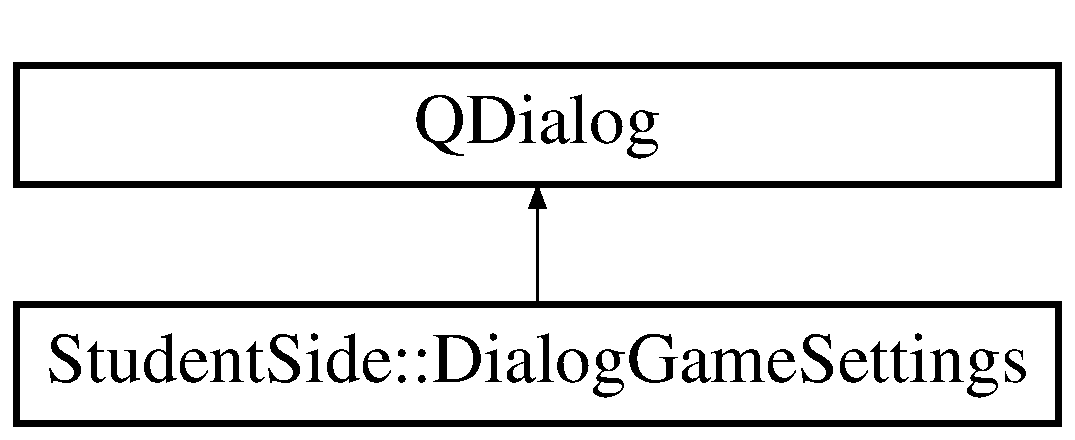
\includegraphics[height=2.000000cm]{class_student_side_1_1_dialog_game_settings}
\end{center}
\end{figure}
\subsection*{Public Slots}
\begin{DoxyCompactItemize}
\item 
void \hyperlink{class_student_side_1_1_dialog_game_settings_a9ee703736f4cde7137c785f00b0bc4d9}{normal} ()
\begin{DoxyCompactList}\small\item\em normal game \end{DoxyCompactList}\item 
void \hyperlink{class_student_side_1_1_dialog_game_settings_adce8f9e27b998911d35526350932c95a}{infinite} ()
\begin{DoxyCompactList}\small\item\em infinite time game \end{DoxyCompactList}\item 
void \hyperlink{class_student_side_1_1_dialog_game_settings_a1af75c606fddb4f29189c5cb65a4aa32}{set\-State1min} ()
\begin{DoxyCompactList}\small\item\em set\-State1min changes state of checkbox1min \end{DoxyCompactList}\item 
void \hyperlink{class_student_side_1_1_dialog_game_settings_ad8ddebcb7566ee6ee9abe7463659ce0b}{set\-State2min} ()
\begin{DoxyCompactList}\small\item\em set\-State2minc hanges state of checkbox2min \end{DoxyCompactList}\end{DoxyCompactItemize}
\subsection*{Signals}
\begin{DoxyCompactItemize}
\item 
void \hyperlink{class_student_side_1_1_dialog_game_settings_a17dedd787d5e757bcf6ac098e91938ed}{normal\-Settings} (Q\-String name, int timelimit)
\begin{DoxyCompactList}\small\item\em normal\-Settings to set normal game settings \end{DoxyCompactList}\item 
void \hyperlink{class_student_side_1_1_dialog_game_settings_ae6867086738b0a74b518d9683539dbe8}{infinite\-Settings} (Q\-String name)
\begin{DoxyCompactList}\small\item\em infinite\-Settings to set infinite time game. \end{DoxyCompactList}\end{DoxyCompactItemize}
\subsection*{Public Member Functions}
\begin{DoxyCompactItemize}
\item 
\hyperlink{class_student_side_1_1_dialog_game_settings_a862ee1ef85f8343eddc675b6737b3a39}{Dialog\-Game\-Settings} (Q\-Widget $\ast$parent=nullptr)
\begin{DoxyCompactList}\small\item\em \hyperlink{class_student_side_1_1_dialog_game_settings}{Dialog\-Game\-Settings} constructor for the dialog window. \end{DoxyCompactList}\item 
\hyperlink{class_student_side_1_1_dialog_game_settings_a1830c64fa4518461ce233aaff1674107}{$\sim$\-Dialog\-Game\-Settings} ()
\begin{DoxyCompactList}\small\item\em Destructor. \end{DoxyCompactList}\end{DoxyCompactItemize}


\subsection{Detailed Description}
The Dialog\-Gane\-Settings class sets up dialog window to get pre settings for the main game. 

\subsection{Constructor \& Destructor Documentation}
\hypertarget{class_student_side_1_1_dialog_game_settings_a862ee1ef85f8343eddc675b6737b3a39}{\index{Student\-Side\-::\-Dialog\-Game\-Settings@{Student\-Side\-::\-Dialog\-Game\-Settings}!Dialog\-Game\-Settings@{Dialog\-Game\-Settings}}
\index{Dialog\-Game\-Settings@{Dialog\-Game\-Settings}!StudentSide::DialogGameSettings@{Student\-Side\-::\-Dialog\-Game\-Settings}}
\subsubsection[{Dialog\-Game\-Settings}]{\setlength{\rightskip}{0pt plus 5cm}Student\-Side\-::\-Dialog\-Game\-Settings\-::\-Dialog\-Game\-Settings (
\begin{DoxyParamCaption}
\item[{Q\-Widget $\ast$}]{parent = {\ttfamily nullptr}}
\end{DoxyParamCaption}
)\hspace{0.3cm}{\ttfamily [explicit]}}}\label{class_student_side_1_1_dialog_game_settings_a862ee1ef85f8343eddc675b6737b3a39}


\hyperlink{class_student_side_1_1_dialog_game_settings}{Dialog\-Game\-Settings} constructor for the dialog window. 


\begin{DoxyParams}{Parameters}
{\em parent} & \\
\hline
\end{DoxyParams}
\hypertarget{class_student_side_1_1_dialog_game_settings_a1830c64fa4518461ce233aaff1674107}{\index{Student\-Side\-::\-Dialog\-Game\-Settings@{Student\-Side\-::\-Dialog\-Game\-Settings}!$\sim$\-Dialog\-Game\-Settings@{$\sim$\-Dialog\-Game\-Settings}}
\index{$\sim$\-Dialog\-Game\-Settings@{$\sim$\-Dialog\-Game\-Settings}!StudentSide::DialogGameSettings@{Student\-Side\-::\-Dialog\-Game\-Settings}}
\subsubsection[{$\sim$\-Dialog\-Game\-Settings}]{\setlength{\rightskip}{0pt plus 5cm}Student\-Side\-::\-Dialog\-Game\-Settings\-::$\sim$\-Dialog\-Game\-Settings (
\begin{DoxyParamCaption}
{}
\end{DoxyParamCaption}
)}}\label{class_student_side_1_1_dialog_game_settings_a1830c64fa4518461ce233aaff1674107}


Destructor. 

\begin{DoxyPrecond}{Precondition}
-\/ 
\end{DoxyPrecond}


\subsection{Member Function Documentation}
\hypertarget{class_student_side_1_1_dialog_game_settings_adce8f9e27b998911d35526350932c95a}{\index{Student\-Side\-::\-Dialog\-Game\-Settings@{Student\-Side\-::\-Dialog\-Game\-Settings}!infinite@{infinite}}
\index{infinite@{infinite}!StudentSide::DialogGameSettings@{Student\-Side\-::\-Dialog\-Game\-Settings}}
\subsubsection[{infinite}]{\setlength{\rightskip}{0pt plus 5cm}void Student\-Side\-::\-Dialog\-Game\-Settings\-::infinite (
\begin{DoxyParamCaption}
{}
\end{DoxyParamCaption}
)\hspace{0.3cm}{\ttfamily [slot]}}}\label{class_student_side_1_1_dialog_game_settings_adce8f9e27b998911d35526350932c95a}


infinite time game 

\hypertarget{class_student_side_1_1_dialog_game_settings_ae6867086738b0a74b518d9683539dbe8}{\index{Student\-Side\-::\-Dialog\-Game\-Settings@{Student\-Side\-::\-Dialog\-Game\-Settings}!infinite\-Settings@{infinite\-Settings}}
\index{infinite\-Settings@{infinite\-Settings}!StudentSide::DialogGameSettings@{Student\-Side\-::\-Dialog\-Game\-Settings}}
\subsubsection[{infinite\-Settings}]{\setlength{\rightskip}{0pt plus 5cm}void Student\-Side\-::\-Dialog\-Game\-Settings\-::infinite\-Settings (
\begin{DoxyParamCaption}
\item[{Q\-String}]{name}
\end{DoxyParamCaption}
)\hspace{0.3cm}{\ttfamily [signal]}}}\label{class_student_side_1_1_dialog_game_settings_ae6867086738b0a74b518d9683539dbe8}


infinite\-Settings to set infinite time game. 


\begin{DoxyParams}{Parameters}
{\em name} & Player name \\
\hline
\end{DoxyParams}
\begin{DoxyPrecond}{Precondition}
-\/ 
\end{DoxyPrecond}
\begin{DoxyPostcond}{Postcondition}
Exception guaranteed\-: nothrow 
\end{DoxyPostcond}
\hypertarget{class_student_side_1_1_dialog_game_settings_a9ee703736f4cde7137c785f00b0bc4d9}{\index{Student\-Side\-::\-Dialog\-Game\-Settings@{Student\-Side\-::\-Dialog\-Game\-Settings}!normal@{normal}}
\index{normal@{normal}!StudentSide::DialogGameSettings@{Student\-Side\-::\-Dialog\-Game\-Settings}}
\subsubsection[{normal}]{\setlength{\rightskip}{0pt plus 5cm}void Student\-Side\-::\-Dialog\-Game\-Settings\-::normal (
\begin{DoxyParamCaption}
{}
\end{DoxyParamCaption}
)\hspace{0.3cm}{\ttfamily [slot]}}}\label{class_student_side_1_1_dialog_game_settings_a9ee703736f4cde7137c785f00b0bc4d9}


normal game 

\hypertarget{class_student_side_1_1_dialog_game_settings_a17dedd787d5e757bcf6ac098e91938ed}{\index{Student\-Side\-::\-Dialog\-Game\-Settings@{Student\-Side\-::\-Dialog\-Game\-Settings}!normal\-Settings@{normal\-Settings}}
\index{normal\-Settings@{normal\-Settings}!StudentSide::DialogGameSettings@{Student\-Side\-::\-Dialog\-Game\-Settings}}
\subsubsection[{normal\-Settings}]{\setlength{\rightskip}{0pt plus 5cm}void Student\-Side\-::\-Dialog\-Game\-Settings\-::normal\-Settings (
\begin{DoxyParamCaption}
\item[{Q\-String}]{name, }
\item[{int}]{timelimit}
\end{DoxyParamCaption}
)\hspace{0.3cm}{\ttfamily [signal]}}}\label{class_student_side_1_1_dialog_game_settings_a17dedd787d5e757bcf6ac098e91938ed}


normal\-Settings to set normal game settings 


\begin{DoxyParams}{Parameters}
{\em name} & Name of the player \\
\hline
{\em timelimit} & Sets the timelimit for game \\
\hline
\end{DoxyParams}
\begin{DoxyPrecond}{Precondition}
name must be Q\-String and timelimit int 
\end{DoxyPrecond}
\begin{DoxyPostcond}{Postcondition}
Exception guaranteed\-: nothrow 
\end{DoxyPostcond}
\hypertarget{class_student_side_1_1_dialog_game_settings_a1af75c606fddb4f29189c5cb65a4aa32}{\index{Student\-Side\-::\-Dialog\-Game\-Settings@{Student\-Side\-::\-Dialog\-Game\-Settings}!set\-State1min@{set\-State1min}}
\index{set\-State1min@{set\-State1min}!StudentSide::DialogGameSettings@{Student\-Side\-::\-Dialog\-Game\-Settings}}
\subsubsection[{set\-State1min}]{\setlength{\rightskip}{0pt plus 5cm}void Student\-Side\-::\-Dialog\-Game\-Settings\-::set\-State1min (
\begin{DoxyParamCaption}
{}
\end{DoxyParamCaption}
)\hspace{0.3cm}{\ttfamily [slot]}}}\label{class_student_side_1_1_dialog_game_settings_a1af75c606fddb4f29189c5cb65a4aa32}


set\-State1min changes state of checkbox1min 

\hypertarget{class_student_side_1_1_dialog_game_settings_ad8ddebcb7566ee6ee9abe7463659ce0b}{\index{Student\-Side\-::\-Dialog\-Game\-Settings@{Student\-Side\-::\-Dialog\-Game\-Settings}!set\-State2min@{set\-State2min}}
\index{set\-State2min@{set\-State2min}!StudentSide::DialogGameSettings@{Student\-Side\-::\-Dialog\-Game\-Settings}}
\subsubsection[{set\-State2min}]{\setlength{\rightskip}{0pt plus 5cm}void Student\-Side\-::\-Dialog\-Game\-Settings\-::set\-State2min (
\begin{DoxyParamCaption}
{}
\end{DoxyParamCaption}
)\hspace{0.3cm}{\ttfamily [slot]}}}\label{class_student_side_1_1_dialog_game_settings_ad8ddebcb7566ee6ee9abe7463659ce0b}


set\-State2minc hanges state of checkbox2min 



The documentation for this class was generated from the following files\-:\begin{DoxyCompactItemize}
\item 
Game/\hyperlink{dialoggamesettings_8hh}{dialoggamesettings.\-hh}\item 
Game/\hyperlink{dialoggamesettings_8cpp}{dialoggamesettings.\-cpp}\item 
Game/\hyperlink{moc__dialoggamesettings_8cpp}{moc\-\_\-dialoggamesettings.\-cpp}\end{DoxyCompactItemize}

\hypertarget{class_student_side_1_1_game_engine}{\section{Student\-Side\-:\-:Game\-Engine Class Reference}
\label{class_student_side_1_1_game_engine}\index{Student\-Side\-::\-Game\-Engine@{Student\-Side\-::\-Game\-Engine}}
}


The Init\-Game\-Engine class is for setting the game up. It launches dialog window for settings and initializes gamewindow.  




{\ttfamily \#include $<$gameengine.\-hh$>$}

Inheritance diagram for Student\-Side\-:\-:Game\-Engine\-:\begin{figure}[H]
\begin{center}
\leavevmode
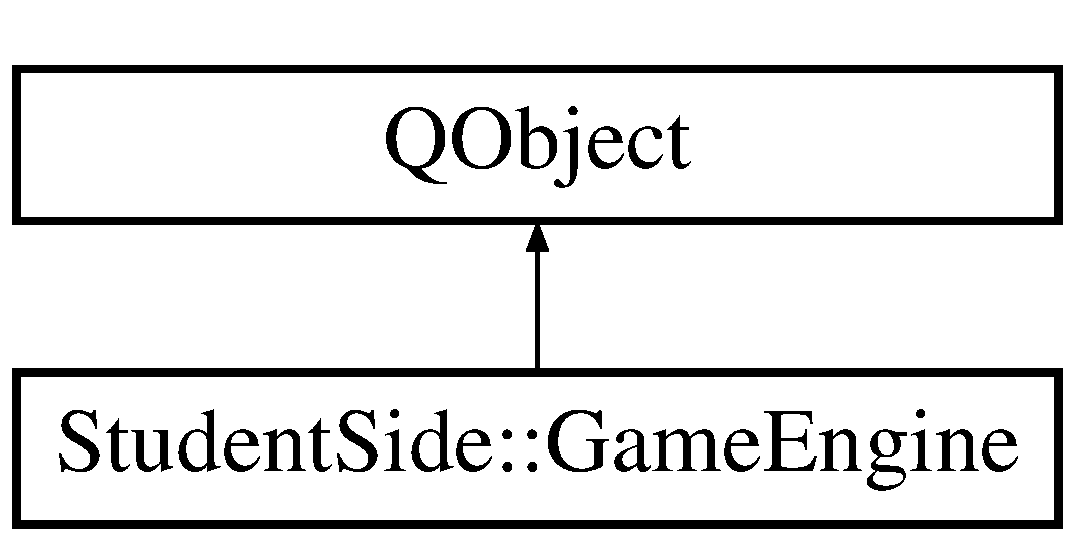
\includegraphics[height=2.000000cm]{class_student_side_1_1_game_engine}
\end{center}
\end{figure}
\subsection*{Public Member Functions}
\begin{DoxyCompactItemize}
\item 
\hyperlink{class_student_side_1_1_game_engine_a97ed7a110060bf799d7cc72f1444f160}{Game\-Engine} ()
\begin{DoxyCompactList}\small\item\em Constructor that initializes game settings and runs mainwindow. \end{DoxyCompactList}\end{DoxyCompactItemize}


\subsection{Detailed Description}
The Init\-Game\-Engine class is for setting the game up. It launches dialog window for settings and initializes gamewindow. 

\subsection{Constructor \& Destructor Documentation}
\hypertarget{class_student_side_1_1_game_engine_a97ed7a110060bf799d7cc72f1444f160}{\index{Student\-Side\-::\-Game\-Engine@{Student\-Side\-::\-Game\-Engine}!Game\-Engine@{Game\-Engine}}
\index{Game\-Engine@{Game\-Engine}!StudentSide::GameEngine@{Student\-Side\-::\-Game\-Engine}}
\subsubsection[{Game\-Engine}]{\setlength{\rightskip}{0pt plus 5cm}Student\-Side\-::\-Game\-Engine\-::\-Game\-Engine (
\begin{DoxyParamCaption}
{}
\end{DoxyParamCaption}
)}}\label{class_student_side_1_1_game_engine_a97ed7a110060bf799d7cc72f1444f160}


Constructor that initializes game settings and runs mainwindow. 



The documentation for this class was generated from the following files\-:\begin{DoxyCompactItemize}
\item 
\hyperlink{gameengine_8hh}{gameengine.\-hh}\item 
\hyperlink{gameengine_8cpp}{gameengine.\-cpp}\end{DoxyCompactItemize}

\hypertarget{class_student_side_1_1_mainwindow}{\section{Student\-Side\-:\-:Mainwindow Class Reference}
\label{class_student_side_1_1_mainwindow}\index{Student\-Side\-::\-Mainwindow@{Student\-Side\-::\-Mainwindow}}
}


The mainwindow class.  




{\ttfamily \#include $<$mainwindow.\-hh$>$}

Inheritance diagram for Student\-Side\-:\-:Mainwindow\-:\begin{figure}[H]
\begin{center}
\leavevmode
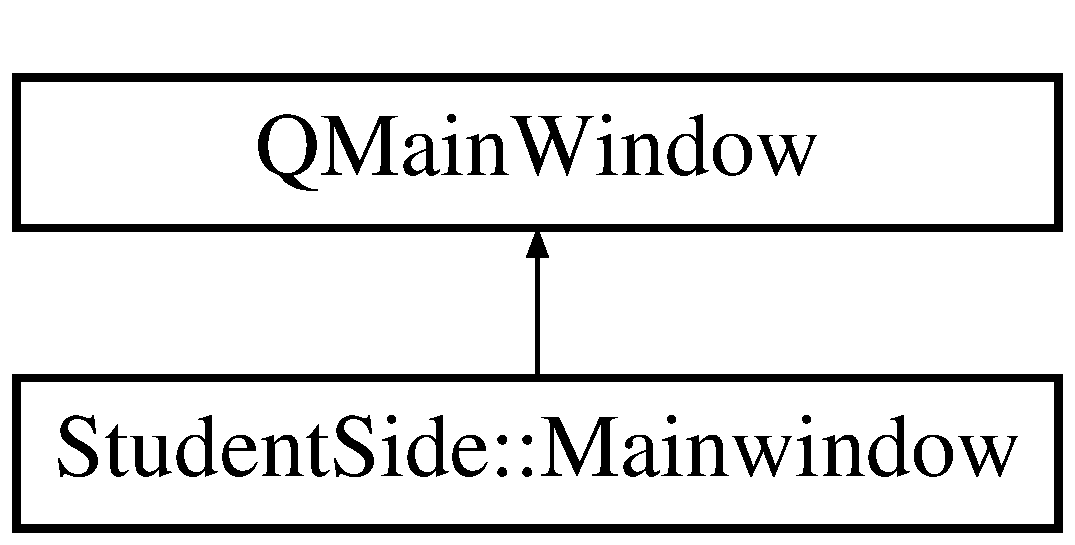
\includegraphics[height=2.000000cm]{class_student_side_1_1_mainwindow}
\end{center}
\end{figure}
\subsection*{Public Member Functions}
\begin{DoxyCompactItemize}
\item 
\hyperlink{class_student_side_1_1_mainwindow_a3be9249fcf6ae0439eab93841d84a4bc}{Mainwindow} (Q\-Widget $\ast$parent=nullptr)
\begin{DoxyCompactList}\small\item\em mainwindow constructor to create mainwindow userinterface. \end{DoxyCompactList}\item 
\hyperlink{class_student_side_1_1_mainwindow_abe12f13a949502ef80a5a4d8a649e410}{$\sim$\-Mainwindow} ()
\begin{DoxyCompactList}\small\item\em Destructor. \end{DoxyCompactList}\item 
void \hyperlink{class_student_side_1_1_mainwindow_a7cc5ee10d853012e479510ee80443d13}{set\-Background} (Q\-Pixmap \&image)
\begin{DoxyCompactList}\small\item\em set\-Background sets the game map to gamewindow \end{DoxyCompactList}\item 
void \hyperlink{class_student_side_1_1_mainwindow_aa6c19fef8cc6731de13b45764277ec67}{add\-Actor} (std\-::shared\-\_\-ptr$<$ Interface\-::\-I\-Actor $>$ actor)
\begin{DoxyCompactList}\small\item\em add\-Actor adds actor to mainwindow \end{DoxyCompactList}\item 
void \hyperlink{class_student_side_1_1_mainwindow_a27478d3419382f2bb8381c7c5af5c8ee}{add\-Stop} (std\-::shared\-\_\-ptr$<$ Interface\-::\-I\-Stop $>$ stop)
\begin{DoxyCompactList}\small\item\em add\-Stop adds bus stop to mainwindow \end{DoxyCompactList}\item 
void \hyperlink{class_student_side_1_1_mainwindow_a7c75210e41e3f9f962b77ebeaaa60811}{move\-Actor} (std\-::shared\-\_\-ptr$<$ Interface\-::\-I\-Actor $>$ actor, int \hyperlink{jquery_8js_a4c3eadaa5164016d2c340d495fc6e55e}{x}, int y)
\begin{DoxyCompactList}\small\item\em move\-Actor moves wanted actor in mainwindow \end{DoxyCompactList}\item 
void \hyperlink{class_student_side_1_1_mainwindow_ada6a000c4e9218c72425bad298e17ed9}{remove\-Actor} (std\-::shared\-\_\-ptr$<$ Interface\-::\-I\-Actor $>$ actor, bool points)
\begin{DoxyCompactList}\small\item\em remove\-Actor removes wanted actor from mainwindow \end{DoxyCompactList}\item 
void \hyperlink{class_student_side_1_1_mainwindow_ad97e4d9dd00a8d0b2b377f749504f98a}{add\-Player} (std\-::shared\-\_\-ptr$<$ \hyperlink{class_student_side_1_1_actor}{Student\-Side\-::\-Actor} $>$ player\-\_\-)
\begin{DoxyCompactList}\small\item\em add\-Player adds player to mainwindow \end{DoxyCompactList}\item 
Interface\-::\-Location \hyperlink{class_student_side_1_1_mainwindow_a487fd2b55286ec6c538c9bfbf8055dfb}{Give\-Player\-Location} ()
\begin{DoxyCompactList}\small\item\em Give\-Player\-Location gives player coordinates. \end{DoxyCompactList}\item 
\hyperlink{class_student_side_1_1player_actor}{Student\-Side\-::player\-Actor} $\ast$ \hyperlink{class_student_side_1_1_mainwindow_aa1eb590a67e0a49fd493c25ec20d189c}{return\-Player} ()
\begin{DoxyCompactList}\small\item\em return\-Player returns player graphics \end{DoxyCompactList}\item 
void \hyperlink{class_student_side_1_1_mainwindow_aed59f49514fa33ffdb6b77b0d0aa54f7}{add\-Points} ()
\begin{DoxyCompactList}\small\item\em add\-Points adds points to points\-\_\-lcd \end{DoxyCompactList}\item 
void \hyperlink{class_student_side_1_1_mainwindow_afa7eb3e3a86fab995d90d253015d3dc7}{take\-Stats} (std\-::shared\-\_\-ptr$<$ \hyperlink{class_student_side_1_1_statistics}{Student\-Side\-::\-Statistics} $>$ stats)
\begin{DoxyCompactList}\small\item\em take\-Stats \end{DoxyCompactList}\item 
Q\-Push\-Button $\ast$ \hyperlink{class_student_side_1_1_mainwindow_a0892eab493aace8eee0358c3d8e88d22}{get\-Start\-Button} ()
\begin{DoxyCompactList}\small\item\em get\-Start\-Button gives start\-Button \end{DoxyCompactList}\item 
Q\-Action $\ast$ \hyperlink{class_student_side_1_1_mainwindow_ae6bc2b06ca8ab22d7e5b5fbc10fbfe3b}{get\-Start\-Action} ()
\begin{DoxyCompactList}\small\item\em get\-Start\-Action return startaction to start the game from menubar \end{DoxyCompactList}\item 
void \hyperlink{class_student_side_1_1_mainwindow_acaa53f081e50381150eae32085f2aeea}{stop\-Game\-Timer} ()
\begin{DoxyCompactList}\small\item\em stop\-Game\-Timer stops game timer in lcd \end{DoxyCompactList}\item 
Q\-Label $\ast$ \hyperlink{class_student_side_1_1_mainwindow_a76f2312aed3a925d44111963a054512a}{get\-People\-Label} ()
\begin{DoxyCompactList}\small\item\em get\-People\-Label returns label containing people info \end{DoxyCompactList}\item 
bool \hyperlink{class_student_side_1_1_mainwindow_a413ff2fac6648addbd19f8a06a1305c7}{game\-Ended} ()
\begin{DoxyCompactList}\small\item\em game\-Ended return boolean if game is ended or not \end{DoxyCompactList}\item 
void \hyperlink{class_student_side_1_1_mainwindow_ace501f039bcececc0c7e891664bbaa50}{destroy\-Player} ()
\begin{DoxyCompactList}\small\item\em destroy\-Player destroys the player \end{DoxyCompactList}\item 
void \hyperlink{class_student_side_1_1_mainwindow_a66eadfc3c6e2f3e893b2142449b00f49}{add\-Nuke} (std\-::shared\-\_\-ptr$<$ \hyperlink{class_student_side_1_1_actor}{Student\-Side\-::\-Actor} $>$ nuke)
\begin{DoxyCompactList}\small\item\em add nuke to game \end{DoxyCompactList}\item 
bool \hyperlink{class_student_side_1_1_mainwindow_a9d393368717ac9f7cbaaae048b355e65}{is\-Nuked} ()
\begin{DoxyCompactList}\small\item\em get information if nuke has been launched by the player \end{DoxyCompactList}\end{DoxyCompactItemize}
\subsection*{Protected Member Functions}
\begin{DoxyCompactItemize}
\item 
void \hyperlink{class_student_side_1_1_mainwindow_a7dbeda19724837043388e76a17280284}{context\-Menu\-Event} (Q\-Context\-Menu\-Event $\ast$event) override
\end{DoxyCompactItemize}


\subsection{Detailed Description}
The mainwindow class. 

\subsection{Constructor \& Destructor Documentation}
\hypertarget{class_student_side_1_1_mainwindow_a3be9249fcf6ae0439eab93841d84a4bc}{\index{Student\-Side\-::\-Mainwindow@{Student\-Side\-::\-Mainwindow}!Mainwindow@{Mainwindow}}
\index{Mainwindow@{Mainwindow}!StudentSide::Mainwindow@{Student\-Side\-::\-Mainwindow}}
\subsubsection[{Mainwindow}]{\setlength{\rightskip}{0pt plus 5cm}Student\-Side\-::\-Mainwindow\-::\-Mainwindow (
\begin{DoxyParamCaption}
\item[{Q\-Widget $\ast$}]{parent = {\ttfamily nullptr}}
\end{DoxyParamCaption}
)\hspace{0.3cm}{\ttfamily [explicit]}}}\label{class_student_side_1_1_mainwindow_a3be9249fcf6ae0439eab93841d84a4bc}


mainwindow constructor to create mainwindow userinterface. 


\begin{DoxyParams}{Parameters}
{\em parent} & \\
\hline
\end{DoxyParams}
\begin{DoxyPrecond}{Precondition}
-\/ 
\end{DoxyPrecond}
\begin{DoxyPostcond}{Postcondition}
Exception guaranteed\-: nothrow 
\end{DoxyPostcond}
\hypertarget{class_student_side_1_1_mainwindow_abe12f13a949502ef80a5a4d8a649e410}{\index{Student\-Side\-::\-Mainwindow@{Student\-Side\-::\-Mainwindow}!$\sim$\-Mainwindow@{$\sim$\-Mainwindow}}
\index{$\sim$\-Mainwindow@{$\sim$\-Mainwindow}!StudentSide::Mainwindow@{Student\-Side\-::\-Mainwindow}}
\subsubsection[{$\sim$\-Mainwindow}]{\setlength{\rightskip}{0pt plus 5cm}Student\-Side\-::\-Mainwindow\-::$\sim$\-Mainwindow (
\begin{DoxyParamCaption}
{}
\end{DoxyParamCaption}
)}}\label{class_student_side_1_1_mainwindow_abe12f13a949502ef80a5a4d8a649e410}


Destructor. 



\subsection{Member Function Documentation}
\hypertarget{class_student_side_1_1_mainwindow_aa6c19fef8cc6731de13b45764277ec67}{\index{Student\-Side\-::\-Mainwindow@{Student\-Side\-::\-Mainwindow}!add\-Actor@{add\-Actor}}
\index{add\-Actor@{add\-Actor}!StudentSide::Mainwindow@{Student\-Side\-::\-Mainwindow}}
\subsubsection[{add\-Actor}]{\setlength{\rightskip}{0pt plus 5cm}void Student\-Side\-::\-Mainwindow\-::add\-Actor (
\begin{DoxyParamCaption}
\item[{std\-::shared\-\_\-ptr$<$ Interface\-::\-I\-Actor $>$}]{actor}
\end{DoxyParamCaption}
)}}\label{class_student_side_1_1_mainwindow_aa6c19fef8cc6731de13b45764277ec67}


add\-Actor adds actor to mainwindow 


\begin{DoxyParams}{Parameters}
{\em actor} & wanted actor to be added \\
\hline
\end{DoxyParams}
\begin{DoxyPrecond}{Precondition}
actor cant be null when addingt it 
\end{DoxyPrecond}
\begin{DoxyPostcond}{Postcondition}
Exception guaranteed\-: nothrow 
\end{DoxyPostcond}
\hypertarget{class_student_side_1_1_mainwindow_a66eadfc3c6e2f3e893b2142449b00f49}{\index{Student\-Side\-::\-Mainwindow@{Student\-Side\-::\-Mainwindow}!add\-Nuke@{add\-Nuke}}
\index{add\-Nuke@{add\-Nuke}!StudentSide::Mainwindow@{Student\-Side\-::\-Mainwindow}}
\subsubsection[{add\-Nuke}]{\setlength{\rightskip}{0pt plus 5cm}void Student\-Side\-::\-Mainwindow\-::add\-Nuke (
\begin{DoxyParamCaption}
\item[{std\-::shared\-\_\-ptr$<$ {\bf Student\-Side\-::\-Actor} $>$}]{nuke}
\end{DoxyParamCaption}
)}}\label{class_student_side_1_1_mainwindow_a66eadfc3c6e2f3e893b2142449b00f49}


add nuke to game 


\begin{DoxyParams}{Parameters}
{\em actor} & for nuke \\
\hline
\end{DoxyParams}
\begin{DoxyPrecond}{Precondition}
nuke must be found \-:D 
\end{DoxyPrecond}
\begin{DoxyPostcond}{Postcondition}
Exception guaranteed\-: nothrow 
\end{DoxyPostcond}
\hypertarget{class_student_side_1_1_mainwindow_ad97e4d9dd00a8d0b2b377f749504f98a}{\index{Student\-Side\-::\-Mainwindow@{Student\-Side\-::\-Mainwindow}!add\-Player@{add\-Player}}
\index{add\-Player@{add\-Player}!StudentSide::Mainwindow@{Student\-Side\-::\-Mainwindow}}
\subsubsection[{add\-Player}]{\setlength{\rightskip}{0pt plus 5cm}void Student\-Side\-::\-Mainwindow\-::add\-Player (
\begin{DoxyParamCaption}
\item[{std\-::shared\-\_\-ptr$<$ {\bf Student\-Side\-::\-Actor} $>$}]{player\-\_\-}
\end{DoxyParamCaption}
)}}\label{class_student_side_1_1_mainwindow_ad97e4d9dd00a8d0b2b377f749504f98a}


add\-Player adds player to mainwindow 


\begin{DoxyParams}{Parameters}
{\em player\-\_\-} & Player that user can move and play with \\
\hline
\end{DoxyParams}
\begin{DoxyPrecond}{Precondition}
player cant be null 
\end{DoxyPrecond}
\begin{DoxyPostcond}{Postcondition}
Exception guaranteed\-: minimum 
\end{DoxyPostcond}
\hypertarget{class_student_side_1_1_mainwindow_aed59f49514fa33ffdb6b77b0d0aa54f7}{\index{Student\-Side\-::\-Mainwindow@{Student\-Side\-::\-Mainwindow}!add\-Points@{add\-Points}}
\index{add\-Points@{add\-Points}!StudentSide::Mainwindow@{Student\-Side\-::\-Mainwindow}}
\subsubsection[{add\-Points}]{\setlength{\rightskip}{0pt plus 5cm}void Student\-Side\-::\-Mainwindow\-::add\-Points (
\begin{DoxyParamCaption}
{}
\end{DoxyParamCaption}
)}}\label{class_student_side_1_1_mainwindow_aed59f49514fa33ffdb6b77b0d0aa54f7}


add\-Points adds points to points\-\_\-lcd 

\begin{DoxyPrecond}{Precondition}
-\/ 
\end{DoxyPrecond}
\begin{DoxyPostcond}{Postcondition}
Exception guaranteed\-: nothrow 
\end{DoxyPostcond}
\hypertarget{class_student_side_1_1_mainwindow_a27478d3419382f2bb8381c7c5af5c8ee}{\index{Student\-Side\-::\-Mainwindow@{Student\-Side\-::\-Mainwindow}!add\-Stop@{add\-Stop}}
\index{add\-Stop@{add\-Stop}!StudentSide::Mainwindow@{Student\-Side\-::\-Mainwindow}}
\subsubsection[{add\-Stop}]{\setlength{\rightskip}{0pt plus 5cm}void Student\-Side\-::\-Mainwindow\-::add\-Stop (
\begin{DoxyParamCaption}
\item[{std\-::shared\-\_\-ptr$<$ Interface\-::\-I\-Stop $>$}]{stop}
\end{DoxyParamCaption}
)}}\label{class_student_side_1_1_mainwindow_a27478d3419382f2bb8381c7c5af5c8ee}


add\-Stop adds bus stop to mainwindow 


\begin{DoxyParams}{Parameters}
{\em stop} & Buss stop to be added \\
\hline
\end{DoxyParams}
\begin{DoxyPrecond}{Precondition}
stop must be found 
\end{DoxyPrecond}
\begin{DoxyPostcond}{Postcondition}
Exception guaranteed\-: nothrow 
\end{DoxyPostcond}
\hypertarget{class_student_side_1_1_mainwindow_a7dbeda19724837043388e76a17280284}{\index{Student\-Side\-::\-Mainwindow@{Student\-Side\-::\-Mainwindow}!context\-Menu\-Event@{context\-Menu\-Event}}
\index{context\-Menu\-Event@{context\-Menu\-Event}!StudentSide::Mainwindow@{Student\-Side\-::\-Mainwindow}}
\subsubsection[{context\-Menu\-Event}]{\setlength{\rightskip}{0pt plus 5cm}void Student\-Side\-::\-Mainwindow\-::context\-Menu\-Event (
\begin{DoxyParamCaption}
\item[{Q\-Context\-Menu\-Event $\ast$}]{event}
\end{DoxyParamCaption}
)\hspace{0.3cm}{\ttfamily [override]}, {\ttfamily [protected]}}}\label{class_student_side_1_1_mainwindow_a7dbeda19724837043388e76a17280284}
\hypertarget{class_student_side_1_1_mainwindow_ace501f039bcececc0c7e891664bbaa50}{\index{Student\-Side\-::\-Mainwindow@{Student\-Side\-::\-Mainwindow}!destroy\-Player@{destroy\-Player}}
\index{destroy\-Player@{destroy\-Player}!StudentSide::Mainwindow@{Student\-Side\-::\-Mainwindow}}
\subsubsection[{destroy\-Player}]{\setlength{\rightskip}{0pt plus 5cm}void Student\-Side\-::\-Mainwindow\-::destroy\-Player (
\begin{DoxyParamCaption}
{}
\end{DoxyParamCaption}
)}}\label{class_student_side_1_1_mainwindow_ace501f039bcececc0c7e891664bbaa50}


destroy\-Player destroys the player 

\begin{DoxyPrecond}{Precondition}
-\/ 
\end{DoxyPrecond}
\begin{DoxyPostcond}{Postcondition}
Exception guaranteed\-: nothrow 
\end{DoxyPostcond}
\hypertarget{class_student_side_1_1_mainwindow_a413ff2fac6648addbd19f8a06a1305c7}{\index{Student\-Side\-::\-Mainwindow@{Student\-Side\-::\-Mainwindow}!game\-Ended@{game\-Ended}}
\index{game\-Ended@{game\-Ended}!StudentSide::Mainwindow@{Student\-Side\-::\-Mainwindow}}
\subsubsection[{game\-Ended}]{\setlength{\rightskip}{0pt plus 5cm}bool Student\-Side\-::\-Mainwindow\-::game\-Ended (
\begin{DoxyParamCaption}
{}
\end{DoxyParamCaption}
)}}\label{class_student_side_1_1_mainwindow_a413ff2fac6648addbd19f8a06a1305c7}


game\-Ended return boolean if game is ended or not 

\begin{DoxyReturn}{Returns}
true when gane has ended, false otherwise 
\end{DoxyReturn}
\begin{DoxyPrecond}{Precondition}
-\/ 
\end{DoxyPrecond}
\begin{DoxyPostcond}{Postcondition}
Exception guaranteed\-: nothrow 
\end{DoxyPostcond}
\hypertarget{class_student_side_1_1_mainwindow_a76f2312aed3a925d44111963a054512a}{\index{Student\-Side\-::\-Mainwindow@{Student\-Side\-::\-Mainwindow}!get\-People\-Label@{get\-People\-Label}}
\index{get\-People\-Label@{get\-People\-Label}!StudentSide::Mainwindow@{Student\-Side\-::\-Mainwindow}}
\subsubsection[{get\-People\-Label}]{\setlength{\rightskip}{0pt plus 5cm}Q\-Label $\ast$ Student\-Side\-::\-Mainwindow\-::get\-People\-Label (
\begin{DoxyParamCaption}
{}
\end{DoxyParamCaption}
)}}\label{class_student_side_1_1_mainwindow_a76f2312aed3a925d44111963a054512a}


get\-People\-Label returns label containing people info 

\begin{DoxyReturn}{Returns}
Q\-Label 
\end{DoxyReturn}
\begin{DoxyPrecond}{Precondition}
-\/ 
\end{DoxyPrecond}
\begin{DoxyPostcond}{Postcondition}
Exception guaranteed\-: nothrow 
\end{DoxyPostcond}
\hypertarget{class_student_side_1_1_mainwindow_ae6bc2b06ca8ab22d7e5b5fbc10fbfe3b}{\index{Student\-Side\-::\-Mainwindow@{Student\-Side\-::\-Mainwindow}!get\-Start\-Action@{get\-Start\-Action}}
\index{get\-Start\-Action@{get\-Start\-Action}!StudentSide::Mainwindow@{Student\-Side\-::\-Mainwindow}}
\subsubsection[{get\-Start\-Action}]{\setlength{\rightskip}{0pt plus 5cm}Q\-Action $\ast$ Student\-Side\-::\-Mainwindow\-::get\-Start\-Action (
\begin{DoxyParamCaption}
{}
\end{DoxyParamCaption}
)}}\label{class_student_side_1_1_mainwindow_ae6bc2b06ca8ab22d7e5b5fbc10fbfe3b}


get\-Start\-Action return startaction to start the game from menubar 

\begin{DoxyReturn}{Returns}
star\-Action 
\end{DoxyReturn}
\begin{DoxyPrecond}{Precondition}
-\/ 
\end{DoxyPrecond}
\begin{DoxyPostcond}{Postcondition}
Exception guaranteed\-: nothrow 
\end{DoxyPostcond}
\hypertarget{class_student_side_1_1_mainwindow_a0892eab493aace8eee0358c3d8e88d22}{\index{Student\-Side\-::\-Mainwindow@{Student\-Side\-::\-Mainwindow}!get\-Start\-Button@{get\-Start\-Button}}
\index{get\-Start\-Button@{get\-Start\-Button}!StudentSide::Mainwindow@{Student\-Side\-::\-Mainwindow}}
\subsubsection[{get\-Start\-Button}]{\setlength{\rightskip}{0pt plus 5cm}Q\-Push\-Button $\ast$ Student\-Side\-::\-Mainwindow\-::get\-Start\-Button (
\begin{DoxyParamCaption}
{}
\end{DoxyParamCaption}
)}}\label{class_student_side_1_1_mainwindow_a0892eab493aace8eee0358c3d8e88d22}


get\-Start\-Button gives start\-Button 

\begin{DoxyReturn}{Returns}
star\-Button of userinterface 
\end{DoxyReturn}
\begin{DoxyPrecond}{Precondition}
-\/ 
\end{DoxyPrecond}
\begin{DoxyPostcond}{Postcondition}
Exception guaranteed\-: nothrow 
\end{DoxyPostcond}
\hypertarget{class_student_side_1_1_mainwindow_a487fd2b55286ec6c538c9bfbf8055dfb}{\index{Student\-Side\-::\-Mainwindow@{Student\-Side\-::\-Mainwindow}!Give\-Player\-Location@{Give\-Player\-Location}}
\index{Give\-Player\-Location@{Give\-Player\-Location}!StudentSide::Mainwindow@{Student\-Side\-::\-Mainwindow}}
\subsubsection[{Give\-Player\-Location}]{\setlength{\rightskip}{0pt plus 5cm}Interface\-::\-Location Student\-Side\-::\-Mainwindow\-::\-Give\-Player\-Location (
\begin{DoxyParamCaption}
{}
\end{DoxyParamCaption}
)}}\label{class_student_side_1_1_mainwindow_a487fd2b55286ec6c538c9bfbf8055dfb}


Give\-Player\-Location gives player coordinates. 

\begin{DoxyReturn}{Returns}
location of player 
\end{DoxyReturn}
\hypertarget{class_student_side_1_1_mainwindow_a9d393368717ac9f7cbaaae048b355e65}{\index{Student\-Side\-::\-Mainwindow@{Student\-Side\-::\-Mainwindow}!is\-Nuked@{is\-Nuked}}
\index{is\-Nuked@{is\-Nuked}!StudentSide::Mainwindow@{Student\-Side\-::\-Mainwindow}}
\subsubsection[{is\-Nuked}]{\setlength{\rightskip}{0pt plus 5cm}bool Student\-Side\-::\-Mainwindow\-::is\-Nuked (
\begin{DoxyParamCaption}
{}
\end{DoxyParamCaption}
)}}\label{class_student_side_1_1_mainwindow_a9d393368717ac9f7cbaaae048b355e65}


get information if nuke has been launched by the player 

\begin{DoxyPrecond}{Precondition}
-\/ 
\end{DoxyPrecond}
\begin{DoxyPostcond}{Postcondition}
Exception guaranteed\-: minimum 
\end{DoxyPostcond}
\hypertarget{class_student_side_1_1_mainwindow_a7c75210e41e3f9f962b77ebeaaa60811}{\index{Student\-Side\-::\-Mainwindow@{Student\-Side\-::\-Mainwindow}!move\-Actor@{move\-Actor}}
\index{move\-Actor@{move\-Actor}!StudentSide::Mainwindow@{Student\-Side\-::\-Mainwindow}}
\subsubsection[{move\-Actor}]{\setlength{\rightskip}{0pt plus 5cm}void Student\-Side\-::\-Mainwindow\-::move\-Actor (
\begin{DoxyParamCaption}
\item[{std\-::shared\-\_\-ptr$<$ Interface\-::\-I\-Actor $>$}]{actor, }
\item[{int}]{x, }
\item[{int}]{y}
\end{DoxyParamCaption}
)}}\label{class_student_side_1_1_mainwindow_a7c75210e41e3f9f962b77ebeaaa60811}


move\-Actor moves wanted actor in mainwindow 


\begin{DoxyParams}{Parameters}
{\em actor} & \hyperlink{class_student_side_1_1_actor}{Actor} to be moved \\
\hline
{\em x} & x-\/coordinate \\
\hline
{\em y} & y-\/coordinate \\
\hline
\end{DoxyParams}
\begin{DoxyPrecond}{Precondition}
actor must be found and x and y coordinates do not pass map borders 
\end{DoxyPrecond}
\begin{DoxyPostcond}{Postcondition}
Exception guaranteed\-: minimum 
\end{DoxyPostcond}
\hypertarget{class_student_side_1_1_mainwindow_ada6a000c4e9218c72425bad298e17ed9}{\index{Student\-Side\-::\-Mainwindow@{Student\-Side\-::\-Mainwindow}!remove\-Actor@{remove\-Actor}}
\index{remove\-Actor@{remove\-Actor}!StudentSide::Mainwindow@{Student\-Side\-::\-Mainwindow}}
\subsubsection[{remove\-Actor}]{\setlength{\rightskip}{0pt plus 5cm}void Student\-Side\-::\-Mainwindow\-::remove\-Actor (
\begin{DoxyParamCaption}
\item[{std\-::shared\-\_\-ptr$<$ Interface\-::\-I\-Actor $>$}]{actor, }
\item[{bool}]{points}
\end{DoxyParamCaption}
)}}\label{class_student_side_1_1_mainwindow_ada6a000c4e9218c72425bad298e17ed9}


remove\-Actor removes wanted actor from mainwindow 


\begin{DoxyParams}{Parameters}
{\em actor} & \hyperlink{class_student_side_1_1_actor}{Actor} to be removed \\
\hline
\end{DoxyParams}
\begin{DoxyPrecond}{Precondition}
actor must be found 
\end{DoxyPrecond}
\begin{DoxyPostcond}{Postcondition}
Exception guaranteed\-: nothrow 
\end{DoxyPostcond}
\hypertarget{class_student_side_1_1_mainwindow_aa1eb590a67e0a49fd493c25ec20d189c}{\index{Student\-Side\-::\-Mainwindow@{Student\-Side\-::\-Mainwindow}!return\-Player@{return\-Player}}
\index{return\-Player@{return\-Player}!StudentSide::Mainwindow@{Student\-Side\-::\-Mainwindow}}
\subsubsection[{return\-Player}]{\setlength{\rightskip}{0pt plus 5cm}{\bf player\-Actor} $\ast$ Student\-Side\-::\-Mainwindow\-::return\-Player (
\begin{DoxyParamCaption}
{}
\end{DoxyParamCaption}
)}}\label{class_student_side_1_1_mainwindow_aa1eb590a67e0a49fd493c25ec20d189c}


return\-Player returns player graphics 

\begin{DoxyReturn}{Returns}
graphics of player 
\end{DoxyReturn}
\begin{DoxyPrecond}{Precondition}
-\/ 
\end{DoxyPrecond}
\begin{DoxyPostcond}{Postcondition}
Exception guaranteed\-: minimum 
\end{DoxyPostcond}
\hypertarget{class_student_side_1_1_mainwindow_a7cc5ee10d853012e479510ee80443d13}{\index{Student\-Side\-::\-Mainwindow@{Student\-Side\-::\-Mainwindow}!set\-Background@{set\-Background}}
\index{set\-Background@{set\-Background}!StudentSide::Mainwindow@{Student\-Side\-::\-Mainwindow}}
\subsubsection[{set\-Background}]{\setlength{\rightskip}{0pt plus 5cm}void Student\-Side\-::\-Mainwindow\-::set\-Background (
\begin{DoxyParamCaption}
\item[{Q\-Pixmap \&}]{image}
\end{DoxyParamCaption}
)}}\label{class_student_side_1_1_mainwindow_a7cc5ee10d853012e479510ee80443d13}


set\-Background sets the game map to gamewindow 


\begin{DoxyParams}{Parameters}
{\em image} & Map image \\
\hline
\end{DoxyParams}
\begin{DoxyPrecond}{Precondition}
-\/ 
\end{DoxyPrecond}
\begin{DoxyPostcond}{Postcondition}
Exception guaranteed\-: nothrow 
\end{DoxyPostcond}
\hypertarget{class_student_side_1_1_mainwindow_acaa53f081e50381150eae32085f2aeea}{\index{Student\-Side\-::\-Mainwindow@{Student\-Side\-::\-Mainwindow}!stop\-Game\-Timer@{stop\-Game\-Timer}}
\index{stop\-Game\-Timer@{stop\-Game\-Timer}!StudentSide::Mainwindow@{Student\-Side\-::\-Mainwindow}}
\subsubsection[{stop\-Game\-Timer}]{\setlength{\rightskip}{0pt plus 5cm}void Student\-Side\-::\-Mainwindow\-::stop\-Game\-Timer (
\begin{DoxyParamCaption}
{}
\end{DoxyParamCaption}
)}}\label{class_student_side_1_1_mainwindow_acaa53f081e50381150eae32085f2aeea}


stop\-Game\-Timer stops game timer in lcd 

\begin{DoxyPrecond}{Precondition}
-\/ 
\end{DoxyPrecond}
\begin{DoxyPostcond}{Postcondition}
Exception guaranteed\-: nothrow 
\end{DoxyPostcond}
\hypertarget{class_student_side_1_1_mainwindow_afa7eb3e3a86fab995d90d253015d3dc7}{\index{Student\-Side\-::\-Mainwindow@{Student\-Side\-::\-Mainwindow}!take\-Stats@{take\-Stats}}
\index{take\-Stats@{take\-Stats}!StudentSide::Mainwindow@{Student\-Side\-::\-Mainwindow}}
\subsubsection[{take\-Stats}]{\setlength{\rightskip}{0pt plus 5cm}void Student\-Side\-::\-Mainwindow\-::take\-Stats (
\begin{DoxyParamCaption}
\item[{std\-::shared\-\_\-ptr$<$ {\bf Student\-Side\-::\-Statistics} $>$}]{stats}
\end{DoxyParamCaption}
)}}\label{class_student_side_1_1_mainwindow_afa7eb3e3a86fab995d90d253015d3dc7}


take\-Stats 


\begin{DoxyParams}{Parameters}
{\em stats} & \\
\hline
\end{DoxyParams}
\begin{DoxyPrecond}{Precondition}
stats must be found 
\end{DoxyPrecond}
\begin{DoxyPostcond}{Postcondition}
Exception guaranteed\-: nothrow 
\end{DoxyPostcond}


The documentation for this class was generated from the following files\-:\begin{DoxyCompactItemize}
\item 
Game/\hyperlink{mainwindow_8hh}{mainwindow.\-hh}\item 
Game/\hyperlink{mainwindow_8cpp}{mainwindow.\-cpp}\end{DoxyCompactItemize}

\hypertarget{class_student_side_1_1_nuke_actor}{\section{Student\-Side\-:\-:Nuke\-Actor Class Reference}
\label{class_student_side_1_1_nuke_actor}\index{Student\-Side\-::\-Nuke\-Actor@{Student\-Side\-::\-Nuke\-Actor}}
}


The \hyperlink{class_student_side_1_1_nuke_actor}{Nuke\-Actor} class.  




{\ttfamily \#include $<$nukeactor.\-hh$>$}

Inheritance diagram for Student\-Side\-:\-:Nuke\-Actor\-:\begin{figure}[H]
\begin{center}
\leavevmode
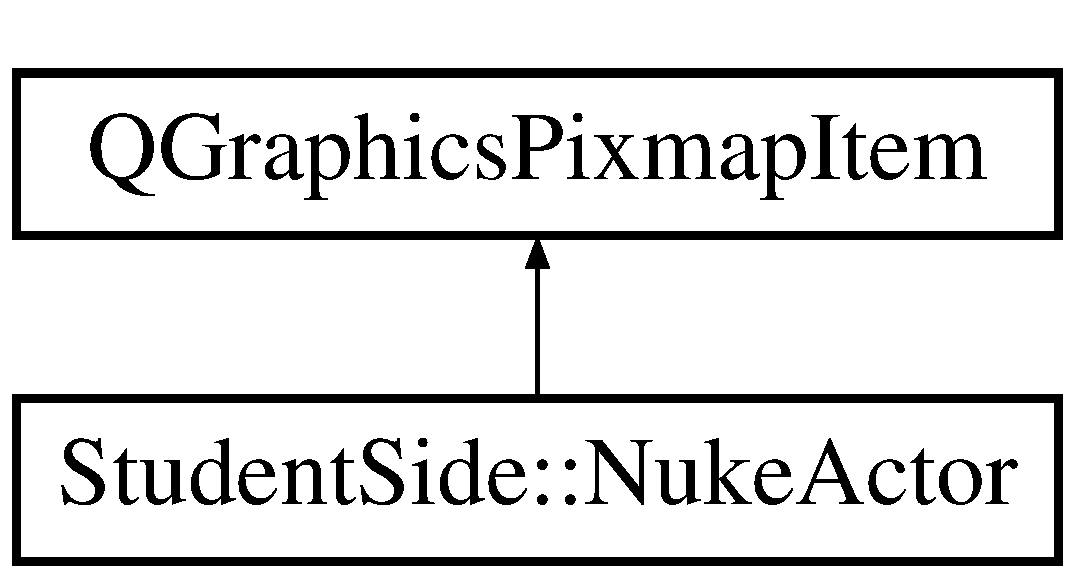
\includegraphics[height=2.000000cm]{class_student_side_1_1_nuke_actor}
\end{center}
\end{figure}
\subsection*{Public Member Functions}
\begin{DoxyCompactItemize}
\item 
\hyperlink{class_student_side_1_1_nuke_actor_abc65d6502333d97c4cd1beb37bdaa163}{Nuke\-Actor} (Interface\-::\-Location location)
\begin{DoxyCompactList}\small\item\em \hyperlink{class_student_side_1_1_nuke_actor}{Nuke\-Actor} gets nukeactor to the map. \end{DoxyCompactList}\item 
\hyperlink{class_student_side_1_1_nuke_actor_a1198514f0e17e36e243b344331c543ac}{$\sim$\-Nuke\-Actor} ()
\begin{DoxyCompactList}\small\item\em Destructor. \end{DoxyCompactList}\end{DoxyCompactItemize}


\subsection{Detailed Description}
The \hyperlink{class_student_side_1_1_nuke_actor}{Nuke\-Actor} class. 

\subsection{Constructor \& Destructor Documentation}
\hypertarget{class_student_side_1_1_nuke_actor_abc65d6502333d97c4cd1beb37bdaa163}{\index{Student\-Side\-::\-Nuke\-Actor@{Student\-Side\-::\-Nuke\-Actor}!Nuke\-Actor@{Nuke\-Actor}}
\index{Nuke\-Actor@{Nuke\-Actor}!StudentSide::NukeActor@{Student\-Side\-::\-Nuke\-Actor}}
\subsubsection[{Nuke\-Actor}]{\setlength{\rightskip}{0pt plus 5cm}Student\-Side\-::\-Nuke\-Actor\-::\-Nuke\-Actor (
\begin{DoxyParamCaption}
\item[{Interface\-::\-Location}]{location}
\end{DoxyParamCaption}
)}}\label{class_student_side_1_1_nuke_actor_abc65d6502333d97c4cd1beb37bdaa163}


\hyperlink{class_student_side_1_1_nuke_actor}{Nuke\-Actor} gets nukeactor to the map. 


\begin{DoxyParams}{Parameters}
{\em location} & Location to draw the nuke actor \\
\hline
\end{DoxyParams}
\begin{DoxyPrecond}{Precondition}
Location must be inside map coordinates 
\end{DoxyPrecond}
\begin{DoxyPostcond}{Postcondition}
Exception guaranteed\-: nothrow 
\end{DoxyPostcond}
\hypertarget{class_student_side_1_1_nuke_actor_a1198514f0e17e36e243b344331c543ac}{\index{Student\-Side\-::\-Nuke\-Actor@{Student\-Side\-::\-Nuke\-Actor}!$\sim$\-Nuke\-Actor@{$\sim$\-Nuke\-Actor}}
\index{$\sim$\-Nuke\-Actor@{$\sim$\-Nuke\-Actor}!StudentSide::NukeActor@{Student\-Side\-::\-Nuke\-Actor}}
\subsubsection[{$\sim$\-Nuke\-Actor}]{\setlength{\rightskip}{0pt plus 5cm}Student\-Side\-::\-Nuke\-Actor\-::$\sim$\-Nuke\-Actor (
\begin{DoxyParamCaption}
{}
\end{DoxyParamCaption}
)}}\label{class_student_side_1_1_nuke_actor_a1198514f0e17e36e243b344331c543ac}


Destructor. 



The documentation for this class was generated from the following files\-:\begin{DoxyCompactItemize}
\item 
Game/\hyperlink{nukeactor_8hh}{nukeactor.\-hh}\item 
Game/\hyperlink{nukeactor_8cpp}{nukeactor.\-cpp}\end{DoxyCompactItemize}

\hypertarget{class_student_side_1_1player_actor}{\section{Student\-Side\-:\-:player\-Actor Class Reference}
\label{class_student_side_1_1player_actor}\index{Student\-Side\-::player\-Actor@{Student\-Side\-::player\-Actor}}
}


{\ttfamily \#include $<$playeractor.\-hh$>$}

Inheritance diagram for Student\-Side\-:\-:player\-Actor\-:\begin{figure}[H]
\begin{center}
\leavevmode
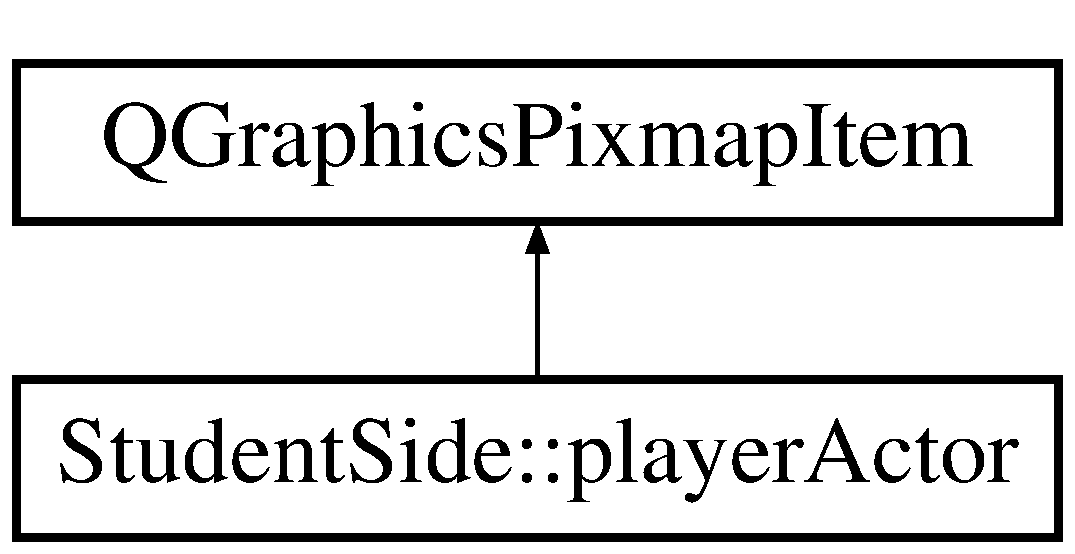
\includegraphics[height=2.000000cm]{class_student_side_1_1player_actor}
\end{center}
\end{figure}
\subsection*{Public Member Functions}
\begin{DoxyCompactItemize}
\item 
\hyperlink{class_student_side_1_1player_actor_a58a39690b97b3442cd7e01a3fae5b8bb}{player\-Actor} (Interface\-::\-Location location)
\begin{DoxyCompactList}\small\item\em \hyperlink{class_student_side_1_1player_actor}{player\-Actor} constructor to set player to map \end{DoxyCompactList}\item 
void \hyperlink{class_student_side_1_1player_actor_a6f2221903208ea8475f4c27efa76e842}{change\-Position} (int \hyperlink{jquery_8js_a4c3eadaa5164016d2c340d495fc6e55e}{x}, int y)
\begin{DoxyCompactList}\small\item\em change\-Position changes players position \end{DoxyCompactList}\item 
void \hyperlink{class_student_side_1_1player_actor_a9feca7b2dd13c5a8febc7c54aac8940e}{key\-Press\-Event} (Q\-Key\-Event $\ast$event) override
\begin{DoxyCompactList}\small\item\em key\-Press\-Event reads keyinputs \end{DoxyCompactList}\item 
Interface\-::\-Location \hyperlink{class_student_side_1_1player_actor_a551fd8c11c43a9ebb0401ed0ee9ef63c}{give\-Location} ()
\begin{DoxyCompactList}\small\item\em give\-Location returns location of player \end{DoxyCompactList}\item 
void \hyperlink{class_student_side_1_1player_actor_a2d1a691ca176eb1436febd320d2040ab}{add\-Nuke} ()
\begin{DoxyCompactList}\small\item\em Marks the nuke to be usable the player. \end{DoxyCompactList}\item 
bool \hyperlink{class_student_side_1_1player_actor_a54888fe10ceb2fdcd7b99e7f5c227da9}{is\-Nuked} ()
\begin{DoxyCompactList}\small\item\em tells if the nuke is used by the player \end{DoxyCompactList}\end{DoxyCompactItemize}


\subsection{Constructor \& Destructor Documentation}
\hypertarget{class_student_side_1_1player_actor_a58a39690b97b3442cd7e01a3fae5b8bb}{\index{Student\-Side\-::player\-Actor@{Student\-Side\-::player\-Actor}!player\-Actor@{player\-Actor}}
\index{player\-Actor@{player\-Actor}!StudentSide::playerActor@{Student\-Side\-::player\-Actor}}
\subsubsection[{player\-Actor}]{\setlength{\rightskip}{0pt plus 5cm}Student\-Side\-::player\-Actor\-::player\-Actor (
\begin{DoxyParamCaption}
\item[{Interface\-::\-Location}]{location}
\end{DoxyParamCaption}
)}}\label{class_student_side_1_1player_actor_a58a39690b97b3442cd7e01a3fae5b8bb}


\hyperlink{class_student_side_1_1player_actor}{player\-Actor} constructor to set player to map 


\begin{DoxyParams}{Parameters}
{\em location} & Location to set player \\
\hline
\end{DoxyParams}
\begin{DoxyPrecond}{Precondition}
Location must be inside map coordinates 
\end{DoxyPrecond}


\subsection{Member Function Documentation}
\hypertarget{class_student_side_1_1player_actor_a2d1a691ca176eb1436febd320d2040ab}{\index{Student\-Side\-::player\-Actor@{Student\-Side\-::player\-Actor}!add\-Nuke@{add\-Nuke}}
\index{add\-Nuke@{add\-Nuke}!StudentSide::playerActor@{Student\-Side\-::player\-Actor}}
\subsubsection[{add\-Nuke}]{\setlength{\rightskip}{0pt plus 5cm}void Student\-Side\-::player\-Actor\-::add\-Nuke (
\begin{DoxyParamCaption}
{}
\end{DoxyParamCaption}
)}}\label{class_student_side_1_1player_actor_a2d1a691ca176eb1436febd320d2040ab}


Marks the nuke to be usable the player. 

\hypertarget{class_student_side_1_1player_actor_a6f2221903208ea8475f4c27efa76e842}{\index{Student\-Side\-::player\-Actor@{Student\-Side\-::player\-Actor}!change\-Position@{change\-Position}}
\index{change\-Position@{change\-Position}!StudentSide::playerActor@{Student\-Side\-::player\-Actor}}
\subsubsection[{change\-Position}]{\setlength{\rightskip}{0pt plus 5cm}void Student\-Side\-::player\-Actor\-::change\-Position (
\begin{DoxyParamCaption}
\item[{int}]{x, }
\item[{int}]{y}
\end{DoxyParamCaption}
)}}\label{class_student_side_1_1player_actor_a6f2221903208ea8475f4c27efa76e842}


change\-Position changes players position 


\begin{DoxyParams}{Parameters}
{\em x} & x-\/coordinate \\
\hline
{\em y} & y-\/coordinate \\
\hline
\end{DoxyParams}
\begin{DoxyPrecond}{Precondition}
Coordinates must be inside map coordinates 
\end{DoxyPrecond}
\hypertarget{class_student_side_1_1player_actor_a551fd8c11c43a9ebb0401ed0ee9ef63c}{\index{Student\-Side\-::player\-Actor@{Student\-Side\-::player\-Actor}!give\-Location@{give\-Location}}
\index{give\-Location@{give\-Location}!StudentSide::playerActor@{Student\-Side\-::player\-Actor}}
\subsubsection[{give\-Location}]{\setlength{\rightskip}{0pt plus 5cm}Interface\-::\-Location Student\-Side\-::player\-Actor\-::give\-Location (
\begin{DoxyParamCaption}
{}
\end{DoxyParamCaption}
)}}\label{class_student_side_1_1player_actor_a551fd8c11c43a9ebb0401ed0ee9ef63c}


give\-Location returns location of player 

\begin{DoxyReturn}{Returns}
location of player 
\end{DoxyReturn}
\hypertarget{class_student_side_1_1player_actor_a54888fe10ceb2fdcd7b99e7f5c227da9}{\index{Student\-Side\-::player\-Actor@{Student\-Side\-::player\-Actor}!is\-Nuked@{is\-Nuked}}
\index{is\-Nuked@{is\-Nuked}!StudentSide::playerActor@{Student\-Side\-::player\-Actor}}
\subsubsection[{is\-Nuked}]{\setlength{\rightskip}{0pt plus 5cm}bool Student\-Side\-::player\-Actor\-::is\-Nuked (
\begin{DoxyParamCaption}
{}
\end{DoxyParamCaption}
)}}\label{class_student_side_1_1player_actor_a54888fe10ceb2fdcd7b99e7f5c227da9}


tells if the nuke is used by the player 

\begin{DoxyReturn}{Returns}
the boolean value of the status of the nuke 
\end{DoxyReturn}
\hypertarget{class_student_side_1_1player_actor_a9feca7b2dd13c5a8febc7c54aac8940e}{\index{Student\-Side\-::player\-Actor@{Student\-Side\-::player\-Actor}!key\-Press\-Event@{key\-Press\-Event}}
\index{key\-Press\-Event@{key\-Press\-Event}!StudentSide::playerActor@{Student\-Side\-::player\-Actor}}
\subsubsection[{key\-Press\-Event}]{\setlength{\rightskip}{0pt plus 5cm}void Student\-Side\-::player\-Actor\-::key\-Press\-Event (
\begin{DoxyParamCaption}
\item[{Q\-Key\-Event $\ast$}]{event}
\end{DoxyParamCaption}
)\hspace{0.3cm}{\ttfamily [override]}}}\label{class_student_side_1_1player_actor_a9feca7b2dd13c5a8febc7c54aac8940e}


key\-Press\-Event reads keyinputs 


\begin{DoxyParams}{Parameters}
{\em event} & from key presses \\
\hline
\end{DoxyParams}


The documentation for this class was generated from the following files\-:\begin{DoxyCompactItemize}
\item 
Game/\hyperlink{playeractor_8hh}{playeractor.\-hh}\item 
Game/\hyperlink{playeractor_8cpp}{playeractor.\-cpp}\end{DoxyCompactItemize}

\hypertarget{class_student_side_1_1_statistics}{\section{Student\-Side\-:\-:Statistics Class Reference}
\label{class_student_side_1_1_statistics}\index{Student\-Side\-::\-Statistics@{Student\-Side\-::\-Statistics}}
}


{\ttfamily \#include $<$statistics.\-hh$>$}

Inheritance diagram for Student\-Side\-:\-:Statistics\-:\begin{figure}[H]
\begin{center}
\leavevmode
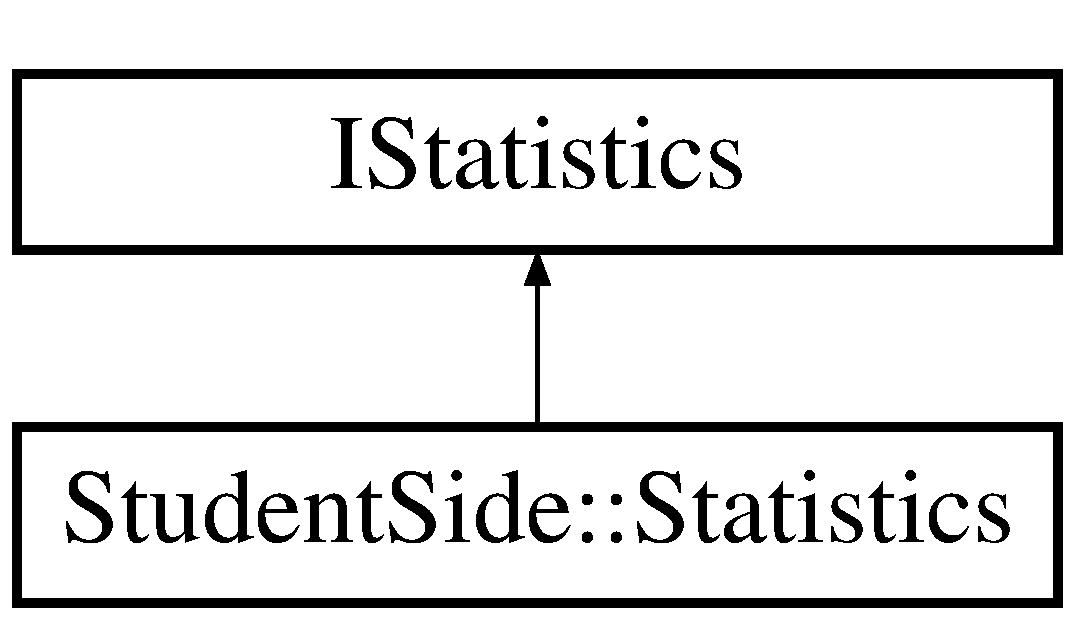
\includegraphics[height=2.000000cm]{class_student_side_1_1_statistics}
\end{center}
\end{figure}
\subsection*{Public Member Functions}
\begin{DoxyCompactItemize}
\item 
\hyperlink{class_student_side_1_1_statistics_a72567fde7744c67397c116f16fe57aed}{Statistics} ()
\begin{DoxyCompactList}\small\item\em \hyperlink{class_student_side_1_1_statistics}{Statistics} contructor. \end{DoxyCompactList}\item 
\hyperlink{class_student_side_1_1_statistics_aa49cd3fc5b2a5c4de8eea5ed690ffb77}{$\sim$\-Statistics} ()
\begin{DoxyCompactList}\small\item\em Destructor. \end{DoxyCompactList}\item 
void \hyperlink{class_student_side_1_1_statistics_a28c61977ebb56858f1cfe02ea58e22a5}{more\-Passengers} (int num) override
\begin{DoxyCompactList}\small\item\em Notifies for the player if new passengers have been added to the game. \end{DoxyCompactList}\item 
void \hyperlink{class_student_side_1_1_statistics_a95d0c05379ea6127c5d60b329e57bb97}{nysse\-Removed} () override
\begin{DoxyCompactList}\small\item\em Notifies for the player if nysse has been removed. \end{DoxyCompactList}\item 
void \hyperlink{class_student_side_1_1_statistics_af7fbe87b0c1ae4bab650ba8c53a3f677}{new\-Nysse} () override
\begin{DoxyCompactList}\small\item\em Notifies for the player if new nysse is added to the game. \end{DoxyCompactList}\item 
void \hyperlink{class_student_side_1_1_statistics_a2d7ba3c86539914571f493736d274ef0}{nysse\-Left} () override
\begin{DoxyCompactList}\small\item\em Notifies for the player if nysse has left the game area. \end{DoxyCompactList}\item 
void \hyperlink{class_student_side_1_1_statistics_ac111b2a2a9fc04b344eee9976c141d41}{Addpoints} (std\-::shared\-\_\-ptr$<$ Interface\-::\-I\-Actor $>$ actor)
\begin{DoxyCompactList}\small\item\em adds points according to which actor has been removed \end{DoxyCompactList}\item 
int \hyperlink{class_student_side_1_1_statistics_a81dff48a0178f5f66c0b01def8afd788}{give\-Current\-Points} ()
\begin{DoxyCompactList}\small\item\em gives the current points to the mainwindow \end{DoxyCompactList}\item 
int \hyperlink{class_student_side_1_1_statistics_a1578ba18299802cc369d14ea5a907a7b}{give\-Passengers} ()
\begin{DoxyCompactList}\small\item\em gives the amount of passengers removed by the player \end{DoxyCompactList}\item 
int \hyperlink{class_student_side_1_1_statistics_a55a744cc3456dad9d43679bab3b4662b}{give\-Nysses} ()
\begin{DoxyCompactList}\small\item\em gives the amount of nysses removed by the player \end{DoxyCompactList}\end{DoxyCompactItemize}


\subsection{Constructor \& Destructor Documentation}
\hypertarget{class_student_side_1_1_statistics_a72567fde7744c67397c116f16fe57aed}{\index{Student\-Side\-::\-Statistics@{Student\-Side\-::\-Statistics}!Statistics@{Statistics}}
\index{Statistics@{Statistics}!StudentSide::Statistics@{Student\-Side\-::\-Statistics}}
\subsubsection[{Statistics}]{\setlength{\rightskip}{0pt plus 5cm}Student\-Side\-::\-Statistics\-::\-Statistics (
\begin{DoxyParamCaption}
{}
\end{DoxyParamCaption}
)}}\label{class_student_side_1_1_statistics_a72567fde7744c67397c116f16fe57aed}


\hyperlink{class_student_side_1_1_statistics}{Statistics} contructor. 

\hypertarget{class_student_side_1_1_statistics_aa49cd3fc5b2a5c4de8eea5ed690ffb77}{\index{Student\-Side\-::\-Statistics@{Student\-Side\-::\-Statistics}!$\sim$\-Statistics@{$\sim$\-Statistics}}
\index{$\sim$\-Statistics@{$\sim$\-Statistics}!StudentSide::Statistics@{Student\-Side\-::\-Statistics}}
\subsubsection[{$\sim$\-Statistics}]{\setlength{\rightskip}{0pt plus 5cm}Student\-Side\-::\-Statistics\-::$\sim$\-Statistics (
\begin{DoxyParamCaption}
{}
\end{DoxyParamCaption}
)}}\label{class_student_side_1_1_statistics_aa49cd3fc5b2a5c4de8eea5ed690ffb77}


Destructor. 



\subsection{Member Function Documentation}
\hypertarget{class_student_side_1_1_statistics_ac111b2a2a9fc04b344eee9976c141d41}{\index{Student\-Side\-::\-Statistics@{Student\-Side\-::\-Statistics}!Addpoints@{Addpoints}}
\index{Addpoints@{Addpoints}!StudentSide::Statistics@{Student\-Side\-::\-Statistics}}
\subsubsection[{Addpoints}]{\setlength{\rightskip}{0pt plus 5cm}void Student\-Side\-::\-Statistics\-::\-Addpoints (
\begin{DoxyParamCaption}
\item[{std\-::shared\-\_\-ptr$<$ Interface\-::\-I\-Actor $>$}]{actor}
\end{DoxyParamCaption}
)}}\label{class_student_side_1_1_statistics_ac111b2a2a9fc04b344eee9976c141d41}


adds points according to which actor has been removed 


\begin{DoxyParams}{Parameters}
{\em actor} & Sharedpointer to Interface of \hyperlink{class_student_side_1_1_actor}{Actor} \\
\hline
\end{DoxyParams}
\begin{DoxyPrecond}{Precondition}
actor is not nullptr 
\end{DoxyPrecond}
\begin{DoxyPostcond}{Postcondition}
Exception guaranteed\-: nothrow 
\end{DoxyPostcond}
\hypertarget{class_student_side_1_1_statistics_a81dff48a0178f5f66c0b01def8afd788}{\index{Student\-Side\-::\-Statistics@{Student\-Side\-::\-Statistics}!give\-Current\-Points@{give\-Current\-Points}}
\index{give\-Current\-Points@{give\-Current\-Points}!StudentSide::Statistics@{Student\-Side\-::\-Statistics}}
\subsubsection[{give\-Current\-Points}]{\setlength{\rightskip}{0pt plus 5cm}int Student\-Side\-::\-Statistics\-::give\-Current\-Points (
\begin{DoxyParamCaption}
{}
\end{DoxyParamCaption}
)}}\label{class_student_side_1_1_statistics_a81dff48a0178f5f66c0b01def8afd788}


gives the current points to the mainwindow 

\begin{DoxyReturn}{Returns}
amount of points saved in variable points 
\end{DoxyReturn}
\begin{DoxyPrecond}{Precondition}
-\/ 
\end{DoxyPrecond}
\begin{DoxyPostcond}{Postcondition}
Exception guaranteed\-: basic 
\end{DoxyPostcond}
\hypertarget{class_student_side_1_1_statistics_a55a744cc3456dad9d43679bab3b4662b}{\index{Student\-Side\-::\-Statistics@{Student\-Side\-::\-Statistics}!give\-Nysses@{give\-Nysses}}
\index{give\-Nysses@{give\-Nysses}!StudentSide::Statistics@{Student\-Side\-::\-Statistics}}
\subsubsection[{give\-Nysses}]{\setlength{\rightskip}{0pt plus 5cm}int Student\-Side\-::\-Statistics\-::give\-Nysses (
\begin{DoxyParamCaption}
{}
\end{DoxyParamCaption}
)}}\label{class_student_side_1_1_statistics_a55a744cc3456dad9d43679bab3b4662b}


gives the amount of nysses removed by the player 

\begin{DoxyReturn}{Returns}
the amount of passengers saved in nysses 
\end{DoxyReturn}
\begin{DoxyPrecond}{Precondition}
-\/ 
\end{DoxyPrecond}
\begin{DoxyPostcond}{Postcondition}
Exception guaranteed\-: basic 
\end{DoxyPostcond}
\hypertarget{class_student_side_1_1_statistics_a1578ba18299802cc369d14ea5a907a7b}{\index{Student\-Side\-::\-Statistics@{Student\-Side\-::\-Statistics}!give\-Passengers@{give\-Passengers}}
\index{give\-Passengers@{give\-Passengers}!StudentSide::Statistics@{Student\-Side\-::\-Statistics}}
\subsubsection[{give\-Passengers}]{\setlength{\rightskip}{0pt plus 5cm}int Student\-Side\-::\-Statistics\-::give\-Passengers (
\begin{DoxyParamCaption}
{}
\end{DoxyParamCaption}
)}}\label{class_student_side_1_1_statistics_a1578ba18299802cc369d14ea5a907a7b}


gives the amount of passengers removed by the player 

\begin{DoxyReturn}{Returns}
the amount of passengers saved in passengers 
\end{DoxyReturn}
\begin{DoxyPrecond}{Precondition}
-\/ 
\end{DoxyPrecond}
\begin{DoxyPostcond}{Postcondition}
Exception guaranteed\-: basic 
\end{DoxyPostcond}
\hypertarget{class_student_side_1_1_statistics_a28c61977ebb56858f1cfe02ea58e22a5}{\index{Student\-Side\-::\-Statistics@{Student\-Side\-::\-Statistics}!more\-Passengers@{more\-Passengers}}
\index{more\-Passengers@{more\-Passengers}!StudentSide::Statistics@{Student\-Side\-::\-Statistics}}
\subsubsection[{more\-Passengers}]{\setlength{\rightskip}{0pt plus 5cm}void Student\-Side\-::\-Statistics\-::more\-Passengers (
\begin{DoxyParamCaption}
\item[{int}]{num}
\end{DoxyParamCaption}
)\hspace{0.3cm}{\ttfamily [override]}}}\label{class_student_side_1_1_statistics_a28c61977ebb56858f1cfe02ea58e22a5}


Notifies for the player if new passengers have been added to the game. 


\begin{DoxyParams}{Parameters}
{\em num} & Number of passengers in the map \\
\hline
\end{DoxyParams}
\begin{DoxyPrecond}{Precondition}
num must be positive value above zero 
\end{DoxyPrecond}
\begin{DoxyPostcond}{Postcondition}
Exception guaranteed\-: nothrow 
\end{DoxyPostcond}
\hypertarget{class_student_side_1_1_statistics_af7fbe87b0c1ae4bab650ba8c53a3f677}{\index{Student\-Side\-::\-Statistics@{Student\-Side\-::\-Statistics}!new\-Nysse@{new\-Nysse}}
\index{new\-Nysse@{new\-Nysse}!StudentSide::Statistics@{Student\-Side\-::\-Statistics}}
\subsubsection[{new\-Nysse}]{\setlength{\rightskip}{0pt plus 5cm}void Student\-Side\-::\-Statistics\-::new\-Nysse (
\begin{DoxyParamCaption}
{}
\end{DoxyParamCaption}
)\hspace{0.3cm}{\ttfamily [override]}}}\label{class_student_side_1_1_statistics_af7fbe87b0c1ae4bab650ba8c53a3f677}


Notifies for the player if new nysse is added to the game. 

\begin{DoxyPrecond}{Precondition}
-\/ 
\end{DoxyPrecond}
\begin{DoxyPostcond}{Postcondition}
Exception guaranteed\-: nothrow 
\end{DoxyPostcond}
\hypertarget{class_student_side_1_1_statistics_a2d7ba3c86539914571f493736d274ef0}{\index{Student\-Side\-::\-Statistics@{Student\-Side\-::\-Statistics}!nysse\-Left@{nysse\-Left}}
\index{nysse\-Left@{nysse\-Left}!StudentSide::Statistics@{Student\-Side\-::\-Statistics}}
\subsubsection[{nysse\-Left}]{\setlength{\rightskip}{0pt plus 5cm}void Student\-Side\-::\-Statistics\-::nysse\-Left (
\begin{DoxyParamCaption}
{}
\end{DoxyParamCaption}
)\hspace{0.3cm}{\ttfamily [override]}}}\label{class_student_side_1_1_statistics_a2d7ba3c86539914571f493736d274ef0}


Notifies for the player if nysse has left the game area. 

\begin{DoxyPrecond}{Precondition}
-\/ 
\end{DoxyPrecond}
\begin{DoxyPostcond}{Postcondition}
Exception guaranteed\-: nothrow 
\end{DoxyPostcond}
\hypertarget{class_student_side_1_1_statistics_a95d0c05379ea6127c5d60b329e57bb97}{\index{Student\-Side\-::\-Statistics@{Student\-Side\-::\-Statistics}!nysse\-Removed@{nysse\-Removed}}
\index{nysse\-Removed@{nysse\-Removed}!StudentSide::Statistics@{Student\-Side\-::\-Statistics}}
\subsubsection[{nysse\-Removed}]{\setlength{\rightskip}{0pt plus 5cm}void Student\-Side\-::\-Statistics\-::nysse\-Removed (
\begin{DoxyParamCaption}
{}
\end{DoxyParamCaption}
)\hspace{0.3cm}{\ttfamily [override]}}}\label{class_student_side_1_1_statistics_a95d0c05379ea6127c5d60b329e57bb97}


Notifies for the player if nysse has been removed. 

\begin{DoxyPrecond}{Precondition}
-\/ 
\end{DoxyPrecond}
\begin{DoxyPostcond}{Postcondition}
Exception guaranteed\-: nothrow 
\end{DoxyPostcond}


The documentation for this class was generated from the following files\-:\begin{DoxyCompactItemize}
\item 
Game/\hyperlink{statistics_8hh}{statistics.\-hh}\item 
Game/\hyperlink{statistics_8cpp}{statistics.\-cpp}\end{DoxyCompactItemize}

\hypertarget{class_student_side_1_1_vehicle}{\section{Student\-Side\-:\-:Vehicle Class Reference}
\label{class_student_side_1_1_vehicle}\index{Student\-Side\-::\-Vehicle@{Student\-Side\-::\-Vehicle}}
}


{\ttfamily \#include $<$vehicle.\-hh$>$}

Inheritance diagram for Student\-Side\-:\-:Vehicle\-:\begin{figure}[H]
\begin{center}
\leavevmode
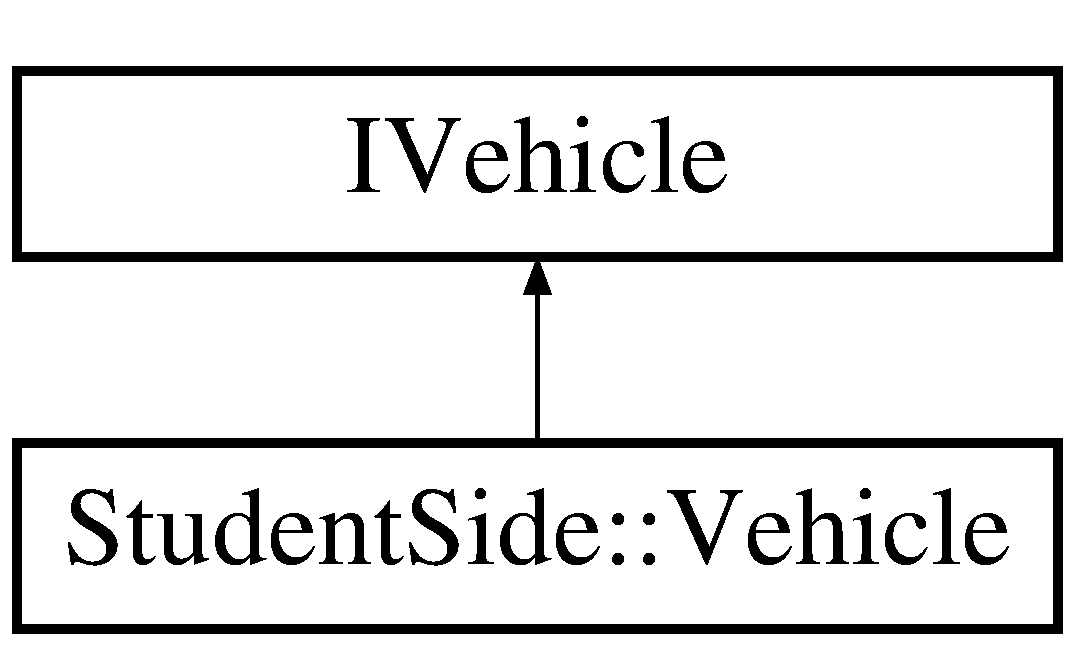
\includegraphics[height=2.000000cm]{class_student_side_1_1_vehicle}
\end{center}
\end{figure}
\subsection*{Public Member Functions}
\begin{DoxyCompactItemize}
\item 
\hyperlink{class_student_side_1_1_vehicle_a0c1ae4b0988ff51bb4ac8f3064e9eb4c}{Vehicle} ()
\begin{DoxyCompactList}\small\item\em \hyperlink{class_student_side_1_1_vehicle}{Vehicle} contructor. \end{DoxyCompactList}\item 
\hyperlink{class_student_side_1_1_vehicle_a3f7640989e79392692aa0cedaa0e4328}{$\sim$\-Vehicle} ()
\begin{DoxyCompactList}\small\item\em Destructor. \end{DoxyCompactList}\item 
std\-::string \hyperlink{class_student_side_1_1_vehicle_afc51d4f1db2c7846f471eba5b03c1d19}{get\-Name} () const override
\begin{DoxyCompactList}\small\item\em get\-Name returns the name of the vehicle \end{DoxyCompactList}\item 
std\-::vector$<$ std\-::shared\-\_\-ptr\\*
$<$ Interface\-::\-I\-Passenger $>$ $>$ \hyperlink{class_student_side_1_1_vehicle_a24c2cece6d5d46979fe9a842d72b06ed}{get\-Passengers} () const override
\begin{DoxyCompactList}\small\item\em get\-Passengers returns vector containing passengers \end{DoxyCompactList}\item 
void \hyperlink{class_student_side_1_1_vehicle_adb754d632a1cfd913adb2fb5862bf376}{add\-Passenger} (std\-::shared\-\_\-ptr$<$ Interface\-::\-I\-Passenger $>$ passenger) override
\begin{DoxyCompactList}\small\item\em add\-Passenger adds passenger to vehicle \end{DoxyCompactList}\item 
void \hyperlink{class_student_side_1_1_vehicle_a6373888a6965dbdb880d8513f9706d60}{remove\-Passenger} (std\-::shared\-\_\-ptr$<$ Interface\-::\-I\-Passenger $>$ passenger) override
\begin{DoxyCompactList}\small\item\em remove\-Passenger removes passenger form vehicle \end{DoxyCompactList}\end{DoxyCompactItemize}


\subsection{Constructor \& Destructor Documentation}
\hypertarget{class_student_side_1_1_vehicle_a0c1ae4b0988ff51bb4ac8f3064e9eb4c}{\index{Student\-Side\-::\-Vehicle@{Student\-Side\-::\-Vehicle}!Vehicle@{Vehicle}}
\index{Vehicle@{Vehicle}!StudentSide::Vehicle@{Student\-Side\-::\-Vehicle}}
\subsubsection[{Vehicle}]{\setlength{\rightskip}{0pt plus 5cm}Student\-Side\-::\-Vehicle\-::\-Vehicle (
\begin{DoxyParamCaption}
{}
\end{DoxyParamCaption}
)}}\label{class_student_side_1_1_vehicle_a0c1ae4b0988ff51bb4ac8f3064e9eb4c}


\hyperlink{class_student_side_1_1_vehicle}{Vehicle} contructor. 

\hypertarget{class_student_side_1_1_vehicle_a3f7640989e79392692aa0cedaa0e4328}{\index{Student\-Side\-::\-Vehicle@{Student\-Side\-::\-Vehicle}!$\sim$\-Vehicle@{$\sim$\-Vehicle}}
\index{$\sim$\-Vehicle@{$\sim$\-Vehicle}!StudentSide::Vehicle@{Student\-Side\-::\-Vehicle}}
\subsubsection[{$\sim$\-Vehicle}]{\setlength{\rightskip}{0pt plus 5cm}Student\-Side\-::\-Vehicle\-::$\sim$\-Vehicle (
\begin{DoxyParamCaption}
{}
\end{DoxyParamCaption}
)}}\label{class_student_side_1_1_vehicle_a3f7640989e79392692aa0cedaa0e4328}


Destructor. 



\subsection{Member Function Documentation}
\hypertarget{class_student_side_1_1_vehicle_adb754d632a1cfd913adb2fb5862bf376}{\index{Student\-Side\-::\-Vehicle@{Student\-Side\-::\-Vehicle}!add\-Passenger@{add\-Passenger}}
\index{add\-Passenger@{add\-Passenger}!StudentSide::Vehicle@{Student\-Side\-::\-Vehicle}}
\subsubsection[{add\-Passenger}]{\setlength{\rightskip}{0pt plus 5cm}void Student\-Side\-::\-Vehicle\-::add\-Passenger (
\begin{DoxyParamCaption}
\item[{std\-::shared\-\_\-ptr$<$ Interface\-::\-I\-Passenger $>$}]{passenger}
\end{DoxyParamCaption}
)\hspace{0.3cm}{\ttfamily [override]}}}\label{class_student_side_1_1_vehicle_adb754d632a1cfd913adb2fb5862bf376}


add\-Passenger adds passenger to vehicle 


\begin{DoxyParams}{Parameters}
{\em passenger} & Passenger actor \\
\hline
\end{DoxyParams}
\begin{DoxyPrecond}{Precondition}
Passenger to be added cannot be null 
\end{DoxyPrecond}
\begin{DoxyPostcond}{Postcondition}
Exception guaranteed\-: minimum 
\end{DoxyPostcond}
\hypertarget{class_student_side_1_1_vehicle_afc51d4f1db2c7846f471eba5b03c1d19}{\index{Student\-Side\-::\-Vehicle@{Student\-Side\-::\-Vehicle}!get\-Name@{get\-Name}}
\index{get\-Name@{get\-Name}!StudentSide::Vehicle@{Student\-Side\-::\-Vehicle}}
\subsubsection[{get\-Name}]{\setlength{\rightskip}{0pt plus 5cm}std\-::string Student\-Side\-::\-Vehicle\-::get\-Name (
\begin{DoxyParamCaption}
{}
\end{DoxyParamCaption}
) const\hspace{0.3cm}{\ttfamily [override]}}}\label{class_student_side_1_1_vehicle_afc51d4f1db2c7846f471eba5b03c1d19}


get\-Name returns the name of the vehicle 

\begin{DoxyReturn}{Returns}
the name of vehicle 
\end{DoxyReturn}
\begin{DoxyPrecond}{Precondition}
-\/ 
\end{DoxyPrecond}
\begin{DoxyPostcond}{Postcondition}
Exception guaranteed\-: basic 
\end{DoxyPostcond}
\hypertarget{class_student_side_1_1_vehicle_a24c2cece6d5d46979fe9a842d72b06ed}{\index{Student\-Side\-::\-Vehicle@{Student\-Side\-::\-Vehicle}!get\-Passengers@{get\-Passengers}}
\index{get\-Passengers@{get\-Passengers}!StudentSide::Vehicle@{Student\-Side\-::\-Vehicle}}
\subsubsection[{get\-Passengers}]{\setlength{\rightskip}{0pt plus 5cm}std\-::vector$<$ std\-::shared\-\_\-ptr$<$ Interface\-::\-I\-Passenger $>$ $>$ Student\-Side\-::\-Vehicle\-::get\-Passengers (
\begin{DoxyParamCaption}
{}
\end{DoxyParamCaption}
) const\hspace{0.3cm}{\ttfamily [override]}}}\label{class_student_side_1_1_vehicle_a24c2cece6d5d46979fe9a842d72b06ed}


get\-Passengers returns vector containing passengers 

\begin{DoxyReturn}{Returns}
vector containing passengers 
\end{DoxyReturn}
\begin{DoxyPrecond}{Precondition}
-\/ 
\end{DoxyPrecond}
\begin{DoxyPostcond}{Postcondition}
Exception guaranteed\-: basic 
\end{DoxyPostcond}
\hypertarget{class_student_side_1_1_vehicle_a6373888a6965dbdb880d8513f9706d60}{\index{Student\-Side\-::\-Vehicle@{Student\-Side\-::\-Vehicle}!remove\-Passenger@{remove\-Passenger}}
\index{remove\-Passenger@{remove\-Passenger}!StudentSide::Vehicle@{Student\-Side\-::\-Vehicle}}
\subsubsection[{remove\-Passenger}]{\setlength{\rightskip}{0pt plus 5cm}void Student\-Side\-::\-Vehicle\-::remove\-Passenger (
\begin{DoxyParamCaption}
\item[{std\-::shared\-\_\-ptr$<$ Interface\-::\-I\-Passenger $>$}]{passenger}
\end{DoxyParamCaption}
)\hspace{0.3cm}{\ttfamily [override]}}}\label{class_student_side_1_1_vehicle_a6373888a6965dbdb880d8513f9706d60}


remove\-Passenger removes passenger form vehicle 


\begin{DoxyParams}{Parameters}
{\em passenger} & \\
\hline
\end{DoxyParams}
\begin{DoxyPrecond}{Precondition}
Passenger to be added cannot be null 
\end{DoxyPrecond}
\begin{DoxyPostcond}{Postcondition}
Exception guaranteed\-: Strong 
\end{DoxyPostcond}


The documentation for this class was generated from the following files\-:\begin{DoxyCompactItemize}
\item 
Game/\hyperlink{vehicle_8hh}{vehicle.\-hh}\item 
Game/\hyperlink{vehicle_8cpp}{vehicle.\-cpp}\end{DoxyCompactItemize}

\chapter{File Documentation}
\hypertarget{actor_8cpp}{\section{actor.\-cpp File Reference}
\label{actor_8cpp}\index{actor.\-cpp@{actor.\-cpp}}
}
{\ttfamily \#include \char`\"{}actor.\-hh\char`\"{}}\\*
\subsection*{Namespaces}
\begin{DoxyCompactItemize}
\item 
\hyperlink{namespace_student_side}{Student\-Side}
\begin{DoxyCompactList}\small\item\em Studenside namespace. \end{DoxyCompactList}\end{DoxyCompactItemize}

\hypertarget{actor_8hh}{\section{actor.\-hh File Reference}
\label{actor_8hh}\index{actor.\-hh@{actor.\-hh}}
}


The Actor class.  


{\ttfamily \#include \char`\"{}interfaces/iactor.\-hh\char`\"{}}\\*
{\ttfamily \#include \char`\"{}core/location.\-hh\char`\"{}}\\*
{\ttfamily \#include \char`\"{}errors/gameerror.\-hh\char`\"{}}\\*
{\ttfamily \#include $<$memory$>$}\\*
\subsection*{Classes}
\begin{DoxyCompactItemize}
\item 
class \hyperlink{class_student_side_1_1_actor}{Student\-Side\-::\-Actor}
\end{DoxyCompactItemize}
\subsection*{Namespaces}
\begin{DoxyCompactItemize}
\item 
\hyperlink{namespace_student_side}{Student\-Side}
\end{DoxyCompactItemize}


\subsection{Detailed Description}
The Actor class. 
\hypertarget{actoritem_8cpp}{\section{Game/actoritem.cpp File Reference}
\label{actoritem_8cpp}\index{Game/actoritem.\-cpp@{Game/actoritem.\-cpp}}
}
{\ttfamily \#include \char`\"{}actoritem.\-hh\char`\"{}}\\*
{\ttfamily \#include $<$Q\-Debug$>$}\\*
{\ttfamily \#include $<$Q\-Image$>$}\\*
{\ttfamily \#include $<$Q\-Pixmap$>$}\\*
{\ttfamily \#include $<$assert.\-h$>$}\\*
\subsection*{Namespaces}
\begin{DoxyCompactItemize}
\item 
\hyperlink{namespace_student_side}{Student\-Side}
\begin{DoxyCompactList}\small\item\em namespace Studen\-Side, Students own imlplementations to project \end{DoxyCompactList}\end{DoxyCompactItemize}

\hypertarget{actoritem_8hh}{\section{actoritem.\-hh File Reference}
\label{actoritem_8hh}\index{actoritem.\-hh@{actoritem.\-hh}}
}


The Actor\-Item class.  


{\ttfamily \#include $<$Q\-Graphics\-Item$>$}\\*
{\ttfamily \#include $<$Q\-Graphics\-Pixmap\-Item$>$}\\*
{\ttfamily \#include $<$Q\-Graphics\-Scene$>$}\\*
{\ttfamily \#include $<$Q\-Painter$>$}\\*
\subsection*{Classes}
\begin{DoxyCompactItemize}
\item 
class \hyperlink{class_student_side_1_1_actor_item}{Student\-Side\-::\-Actor\-Item}
\end{DoxyCompactItemize}
\subsection*{Namespaces}
\begin{DoxyCompactItemize}
\item 
\hyperlink{namespace_student_side}{Student\-Side}
\end{DoxyCompactItemize}
\subsection*{Variables}
\begin{DoxyCompactItemize}
\item 
const Q\-String \hyperlink{actoritem_8hh_aa4b129297bf7c3a2ab33895c4ec37ade}{N\-Y\-S\-S\-E\-\_\-\-S\-T\-O\-P} = \char`\"{}\-:/../pics/pics/Nysse\-Stop.\-png\char`\"{}
\begin{DoxyCompactList}\small\item\em Pic of stopsign. \end{DoxyCompactList}\item 
const Q\-String \hyperlink{actoritem_8hh_aedf8524adc61b4d09d86db4fa2f207d2}{B\-U\-S\-S\-I} = \char`\"{}\-://../pics/pics/bussi.\-png\char`\"{}
\begin{DoxyCompactList}\small\item\em pic of buss \end{DoxyCompactList}\item 
const Q\-String \hyperlink{actoritem_8hh_a919ee1b297d205cded0f0dc03ade1cfd}{H\-U\-M\-A\-N} = \char`\"{}\-://../pics/pics/huma.\-png\char`\"{}
\begin{DoxyCompactList}\small\item\em pic of passenger \end{DoxyCompactList}\item 
const int \hyperlink{actoritem_8hh_abd028a1a48c574e726a4a904fff0a08c}{D\-I\-M\-\_\-\-S\-T\-O\-P} = 10
\item 
const int \hyperlink{actoritem_8hh_a0206546ca28fb9fca0c00861c5843dd5}{D\-I\-M\-\_\-\-B\-U\-S\-S} = 15
\item 
const int \hyperlink{actoritem_8hh_a94bb4115dc75d86789f2424ba4efcbdc}{D\-I\-M\-\_\-\-P\-A\-S\-S\-E\-N\-G\-E\-R} = 30
\item 
const int \hyperlink{actoritem_8hh_a65e7f70d9c573d5bfd13804a406fc067}{B\-U\-S\-S\-\_\-\-S\-T\-O\-P} = 0
\item 
const int \hyperlink{actoritem_8hh_a184d5b62435541e060c4dd4f179bec92}{N\-Y\-S\-S\-E} = 1
\item 
const int \hyperlink{actoritem_8hh_ad93711fcc7685c6b7a6530eda7984a55}{P\-A\-S\-S\-E\-N\-G\-E\-R} = 2
\item 
const int \hyperlink{actoritem_8hh_a9649ab8139c4c2ea5c93625b30d92a05}{W\-I\-D\-T\-H} = 9
\item 
const int \hyperlink{actoritem_8hh_af728b7647e0b8c49832983a31f9a2e9b}{H\-E\-I\-G\-H\-T} = 9
\end{DoxyCompactItemize}


\subsection{Detailed Description}
The Actor\-Item class. 

\subsection{Variable Documentation}
\hypertarget{actoritem_8hh_a65e7f70d9c573d5bfd13804a406fc067}{\index{actoritem.\-hh@{actoritem.\-hh}!B\-U\-S\-S\-\_\-\-S\-T\-O\-P@{B\-U\-S\-S\-\_\-\-S\-T\-O\-P}}
\index{B\-U\-S\-S\-\_\-\-S\-T\-O\-P@{B\-U\-S\-S\-\_\-\-S\-T\-O\-P}!actoritem.hh@{actoritem.\-hh}}
\subsubsection[{B\-U\-S\-S\-\_\-\-S\-T\-O\-P}]{\setlength{\rightskip}{0pt plus 5cm}const int B\-U\-S\-S\-\_\-\-S\-T\-O\-P = 0}}\label{actoritem_8hh_a65e7f70d9c573d5bfd13804a406fc067}
\hypertarget{actoritem_8hh_aedf8524adc61b4d09d86db4fa2f207d2}{\index{actoritem.\-hh@{actoritem.\-hh}!B\-U\-S\-S\-I@{B\-U\-S\-S\-I}}
\index{B\-U\-S\-S\-I@{B\-U\-S\-S\-I}!actoritem.hh@{actoritem.\-hh}}
\subsubsection[{B\-U\-S\-S\-I}]{\setlength{\rightskip}{0pt plus 5cm}const Q\-String B\-U\-S\-S\-I = \char`\"{}\-://../pics/pics/bussi.\-png\char`\"{}}}\label{actoritem_8hh_aedf8524adc61b4d09d86db4fa2f207d2}


pic of buss 

\hypertarget{actoritem_8hh_a0206546ca28fb9fca0c00861c5843dd5}{\index{actoritem.\-hh@{actoritem.\-hh}!D\-I\-M\-\_\-\-B\-U\-S\-S@{D\-I\-M\-\_\-\-B\-U\-S\-S}}
\index{D\-I\-M\-\_\-\-B\-U\-S\-S@{D\-I\-M\-\_\-\-B\-U\-S\-S}!actoritem.hh@{actoritem.\-hh}}
\subsubsection[{D\-I\-M\-\_\-\-B\-U\-S\-S}]{\setlength{\rightskip}{0pt plus 5cm}const int D\-I\-M\-\_\-\-B\-U\-S\-S = 15}}\label{actoritem_8hh_a0206546ca28fb9fca0c00861c5843dd5}
\hypertarget{actoritem_8hh_a94bb4115dc75d86789f2424ba4efcbdc}{\index{actoritem.\-hh@{actoritem.\-hh}!D\-I\-M\-\_\-\-P\-A\-S\-S\-E\-N\-G\-E\-R@{D\-I\-M\-\_\-\-P\-A\-S\-S\-E\-N\-G\-E\-R}}
\index{D\-I\-M\-\_\-\-P\-A\-S\-S\-E\-N\-G\-E\-R@{D\-I\-M\-\_\-\-P\-A\-S\-S\-E\-N\-G\-E\-R}!actoritem.hh@{actoritem.\-hh}}
\subsubsection[{D\-I\-M\-\_\-\-P\-A\-S\-S\-E\-N\-G\-E\-R}]{\setlength{\rightskip}{0pt plus 5cm}const int D\-I\-M\-\_\-\-P\-A\-S\-S\-E\-N\-G\-E\-R = 30}}\label{actoritem_8hh_a94bb4115dc75d86789f2424ba4efcbdc}
\hypertarget{actoritem_8hh_abd028a1a48c574e726a4a904fff0a08c}{\index{actoritem.\-hh@{actoritem.\-hh}!D\-I\-M\-\_\-\-S\-T\-O\-P@{D\-I\-M\-\_\-\-S\-T\-O\-P}}
\index{D\-I\-M\-\_\-\-S\-T\-O\-P@{D\-I\-M\-\_\-\-S\-T\-O\-P}!actoritem.hh@{actoritem.\-hh}}
\subsubsection[{D\-I\-M\-\_\-\-S\-T\-O\-P}]{\setlength{\rightskip}{0pt plus 5cm}const int D\-I\-M\-\_\-\-S\-T\-O\-P = 10}}\label{actoritem_8hh_abd028a1a48c574e726a4a904fff0a08c}
\hypertarget{actoritem_8hh_af728b7647e0b8c49832983a31f9a2e9b}{\index{actoritem.\-hh@{actoritem.\-hh}!H\-E\-I\-G\-H\-T@{H\-E\-I\-G\-H\-T}}
\index{H\-E\-I\-G\-H\-T@{H\-E\-I\-G\-H\-T}!actoritem.hh@{actoritem.\-hh}}
\subsubsection[{H\-E\-I\-G\-H\-T}]{\setlength{\rightskip}{0pt plus 5cm}const int H\-E\-I\-G\-H\-T = 9}}\label{actoritem_8hh_af728b7647e0b8c49832983a31f9a2e9b}
\hypertarget{actoritem_8hh_a919ee1b297d205cded0f0dc03ade1cfd}{\index{actoritem.\-hh@{actoritem.\-hh}!H\-U\-M\-A\-N@{H\-U\-M\-A\-N}}
\index{H\-U\-M\-A\-N@{H\-U\-M\-A\-N}!actoritem.hh@{actoritem.\-hh}}
\subsubsection[{H\-U\-M\-A\-N}]{\setlength{\rightskip}{0pt plus 5cm}const Q\-String H\-U\-M\-A\-N = \char`\"{}\-://../pics/pics/huma.\-png\char`\"{}}}\label{actoritem_8hh_a919ee1b297d205cded0f0dc03ade1cfd}


pic of passenger 

\hypertarget{actoritem_8hh_a184d5b62435541e060c4dd4f179bec92}{\index{actoritem.\-hh@{actoritem.\-hh}!N\-Y\-S\-S\-E@{N\-Y\-S\-S\-E}}
\index{N\-Y\-S\-S\-E@{N\-Y\-S\-S\-E}!actoritem.hh@{actoritem.\-hh}}
\subsubsection[{N\-Y\-S\-S\-E}]{\setlength{\rightskip}{0pt plus 5cm}const int N\-Y\-S\-S\-E = 1}}\label{actoritem_8hh_a184d5b62435541e060c4dd4f179bec92}
\hypertarget{actoritem_8hh_aa4b129297bf7c3a2ab33895c4ec37ade}{\index{actoritem.\-hh@{actoritem.\-hh}!N\-Y\-S\-S\-E\-\_\-\-S\-T\-O\-P@{N\-Y\-S\-S\-E\-\_\-\-S\-T\-O\-P}}
\index{N\-Y\-S\-S\-E\-\_\-\-S\-T\-O\-P@{N\-Y\-S\-S\-E\-\_\-\-S\-T\-O\-P}!actoritem.hh@{actoritem.\-hh}}
\subsubsection[{N\-Y\-S\-S\-E\-\_\-\-S\-T\-O\-P}]{\setlength{\rightskip}{0pt plus 5cm}const Q\-String N\-Y\-S\-S\-E\-\_\-\-S\-T\-O\-P = \char`\"{}\-:/../pics/pics/Nysse\-Stop.\-png\char`\"{}}}\label{actoritem_8hh_aa4b129297bf7c3a2ab33895c4ec37ade}


Pic of stopsign. 

\hypertarget{actoritem_8hh_ad93711fcc7685c6b7a6530eda7984a55}{\index{actoritem.\-hh@{actoritem.\-hh}!P\-A\-S\-S\-E\-N\-G\-E\-R@{P\-A\-S\-S\-E\-N\-G\-E\-R}}
\index{P\-A\-S\-S\-E\-N\-G\-E\-R@{P\-A\-S\-S\-E\-N\-G\-E\-R}!actoritem.hh@{actoritem.\-hh}}
\subsubsection[{P\-A\-S\-S\-E\-N\-G\-E\-R}]{\setlength{\rightskip}{0pt plus 5cm}const int P\-A\-S\-S\-E\-N\-G\-E\-R = 2}}\label{actoritem_8hh_ad93711fcc7685c6b7a6530eda7984a55}
\hypertarget{actoritem_8hh_a9649ab8139c4c2ea5c93625b30d92a05}{\index{actoritem.\-hh@{actoritem.\-hh}!W\-I\-D\-T\-H@{W\-I\-D\-T\-H}}
\index{W\-I\-D\-T\-H@{W\-I\-D\-T\-H}!actoritem.hh@{actoritem.\-hh}}
\subsubsection[{W\-I\-D\-T\-H}]{\setlength{\rightskip}{0pt plus 5cm}const int W\-I\-D\-T\-H = 9}}\label{actoritem_8hh_a9649ab8139c4c2ea5c93625b30d92a05}

\hypertarget{city_8cpp}{\section{city.\-cpp File Reference}
\label{city_8cpp}\index{city.\-cpp@{city.\-cpp}}
}
{\ttfamily \#include \char`\"{}city.\-hh\char`\"{}}\\*
{\ttfamily \#include $<$Q\-Debug$>$}\\*
{\ttfamily \#include $<$vector$>$}\\*
\subsection*{Namespaces}
\begin{DoxyCompactItemize}
\item 
\hyperlink{namespace_student_side}{Student\-Side}
\begin{DoxyCompactList}\small\item\em Studenside namespace. \end{DoxyCompactList}\end{DoxyCompactItemize}

\hypertarget{city_8hh}{\section{Game/city.hh File Reference}
\label{city_8hh}\index{Game/city.\-hh@{Game/city.\-hh}}
}


The City class that defines city operations.  


{\ttfamily \#include \char`\"{}interfaces/icity.\-hh\char`\"{}}\\*
{\ttfamily \#include \char`\"{}mainwindow.\-hh\char`\"{}}\\*
{\ttfamily \#include \char`\"{}actor.\-hh\char`\"{}}\\*
{\ttfamily \#include \char`\"{}vehicle.\-hh\char`\"{}}\\*
{\ttfamily \#include \char`\"{}statistics.\-hh\char`\"{}}\\*
{\ttfamily \#include \char`\"{}errors/gameerror.\-hh\char`\"{}}\\*
{\ttfamily \#include \char`\"{}errors/initerror.\-hh\char`\"{}}\\*
{\ttfamily \#include $<$Q\-Time$>$}\\*
{\ttfamily \#include $<$Q\-Pixmap$>$}\\*
{\ttfamily \#include $<$algorithm$>$}\\*
\subsection*{Classes}
\begin{DoxyCompactItemize}
\item 
class \hyperlink{class_student_side_1_1_city}{Student\-Side\-::\-City}
\end{DoxyCompactItemize}
\subsection*{Namespaces}
\begin{DoxyCompactItemize}
\item 
\hyperlink{namespace_student_side}{Student\-Side}
\begin{DoxyCompactList}\small\item\em namespace Studen\-Side, Students own imlplementations to project \end{DoxyCompactList}\end{DoxyCompactItemize}
\subsection*{Variables}
\begin{DoxyCompactItemize}
\item 
const int \hyperlink{city_8hh_ae64f34fc2d5f71f07cd3b6d6b9518215}{R\-E\-N\-D\-E\-R\-\_\-\-D\-I\-S\-T\-A\-N\-C\-E} = 2000
\item 
const int \hyperlink{city_8hh_ae9a58fdb539145f04f47e77582514552}{P\-A\-S\-S\-E\-N\-G\-E\-R\-\_\-\-R\-E\-N\-D\-E\-R\-\_\-\-M\-I\-N} = -\/500
\item 
const int \hyperlink{city_8hh_a96b3f3c6628cf7255e17e1b12f001e70}{P\-A\-S\-S\-E\-N\-G\-E\-R\-\_\-\-R\-E\-N\-D\-E\-R\-\_\-\-M\-A\-X} = 1050
\item 
const int \hyperlink{city_8hh_aedc95de80b52c2e078fac78e2c7a8df8}{D\-I\-S\-T\-A\-N\-C\-E\-\_\-\-T\-O\-\_\-\-I\-N\-T\-E\-R\-A\-C\-T} = 25
\end{DoxyCompactItemize}


\subsection{Detailed Description}
The City class that defines city operations. 

\subsection{Variable Documentation}
\hypertarget{city_8hh_aedc95de80b52c2e078fac78e2c7a8df8}{\index{city.\-hh@{city.\-hh}!D\-I\-S\-T\-A\-N\-C\-E\-\_\-\-T\-O\-\_\-\-I\-N\-T\-E\-R\-A\-C\-T@{D\-I\-S\-T\-A\-N\-C\-E\-\_\-\-T\-O\-\_\-\-I\-N\-T\-E\-R\-A\-C\-T}}
\index{D\-I\-S\-T\-A\-N\-C\-E\-\_\-\-T\-O\-\_\-\-I\-N\-T\-E\-R\-A\-C\-T@{D\-I\-S\-T\-A\-N\-C\-E\-\_\-\-T\-O\-\_\-\-I\-N\-T\-E\-R\-A\-C\-T}!city.hh@{city.\-hh}}
\subsubsection[{D\-I\-S\-T\-A\-N\-C\-E\-\_\-\-T\-O\-\_\-\-I\-N\-T\-E\-R\-A\-C\-T}]{\setlength{\rightskip}{0pt plus 5cm}const int D\-I\-S\-T\-A\-N\-C\-E\-\_\-\-T\-O\-\_\-\-I\-N\-T\-E\-R\-A\-C\-T = 25}}\label{city_8hh_aedc95de80b52c2e078fac78e2c7a8df8}
\hypertarget{city_8hh_a96b3f3c6628cf7255e17e1b12f001e70}{\index{city.\-hh@{city.\-hh}!P\-A\-S\-S\-E\-N\-G\-E\-R\-\_\-\-R\-E\-N\-D\-E\-R\-\_\-\-M\-A\-X@{P\-A\-S\-S\-E\-N\-G\-E\-R\-\_\-\-R\-E\-N\-D\-E\-R\-\_\-\-M\-A\-X}}
\index{P\-A\-S\-S\-E\-N\-G\-E\-R\-\_\-\-R\-E\-N\-D\-E\-R\-\_\-\-M\-A\-X@{P\-A\-S\-S\-E\-N\-G\-E\-R\-\_\-\-R\-E\-N\-D\-E\-R\-\_\-\-M\-A\-X}!city.hh@{city.\-hh}}
\subsubsection[{P\-A\-S\-S\-E\-N\-G\-E\-R\-\_\-\-R\-E\-N\-D\-E\-R\-\_\-\-M\-A\-X}]{\setlength{\rightskip}{0pt plus 5cm}const int P\-A\-S\-S\-E\-N\-G\-E\-R\-\_\-\-R\-E\-N\-D\-E\-R\-\_\-\-M\-A\-X = 1050}}\label{city_8hh_a96b3f3c6628cf7255e17e1b12f001e70}
\hypertarget{city_8hh_ae9a58fdb539145f04f47e77582514552}{\index{city.\-hh@{city.\-hh}!P\-A\-S\-S\-E\-N\-G\-E\-R\-\_\-\-R\-E\-N\-D\-E\-R\-\_\-\-M\-I\-N@{P\-A\-S\-S\-E\-N\-G\-E\-R\-\_\-\-R\-E\-N\-D\-E\-R\-\_\-\-M\-I\-N}}
\index{P\-A\-S\-S\-E\-N\-G\-E\-R\-\_\-\-R\-E\-N\-D\-E\-R\-\_\-\-M\-I\-N@{P\-A\-S\-S\-E\-N\-G\-E\-R\-\_\-\-R\-E\-N\-D\-E\-R\-\_\-\-M\-I\-N}!city.hh@{city.\-hh}}
\subsubsection[{P\-A\-S\-S\-E\-N\-G\-E\-R\-\_\-\-R\-E\-N\-D\-E\-R\-\_\-\-M\-I\-N}]{\setlength{\rightskip}{0pt plus 5cm}const int P\-A\-S\-S\-E\-N\-G\-E\-R\-\_\-\-R\-E\-N\-D\-E\-R\-\_\-\-M\-I\-N = -\/500}}\label{city_8hh_ae9a58fdb539145f04f47e77582514552}
\hypertarget{city_8hh_ae64f34fc2d5f71f07cd3b6d6b9518215}{\index{city.\-hh@{city.\-hh}!R\-E\-N\-D\-E\-R\-\_\-\-D\-I\-S\-T\-A\-N\-C\-E@{R\-E\-N\-D\-E\-R\-\_\-\-D\-I\-S\-T\-A\-N\-C\-E}}
\index{R\-E\-N\-D\-E\-R\-\_\-\-D\-I\-S\-T\-A\-N\-C\-E@{R\-E\-N\-D\-E\-R\-\_\-\-D\-I\-S\-T\-A\-N\-C\-E}!city.hh@{city.\-hh}}
\subsubsection[{R\-E\-N\-D\-E\-R\-\_\-\-D\-I\-S\-T\-A\-N\-C\-E}]{\setlength{\rightskip}{0pt plus 5cm}const int R\-E\-N\-D\-E\-R\-\_\-\-D\-I\-S\-T\-A\-N\-C\-E = 2000}}\label{city_8hh_ae64f34fc2d5f71f07cd3b6d6b9518215}

\hypertarget{creategame_8cpp}{\section{Game/creategame.cpp File Reference}
\label{creategame_8cpp}\index{Game/creategame.\-cpp@{Game/creategame.\-cpp}}
}
{\ttfamily \#include \char`\"{}creategame.\-hh\char`\"{}}\\*
{\ttfamily \#include \char`\"{}city.\-hh\char`\"{}}\\*
{\ttfamily \#include \char`\"{}Q\-Image\char`\"{}}\\*
{\ttfamily \#include $<$memory$>$}\\*

\hypertarget{dialoggamesettings_8cpp}{\section{dialoggamesettings.\-cpp File Reference}
\label{dialoggamesettings_8cpp}\index{dialoggamesettings.\-cpp@{dialoggamesettings.\-cpp}}
}
{\ttfamily \#include \char`\"{}dialoggamesettings.\-hh\char`\"{}}\\*
{\ttfamily \#include \char`\"{}ui\-\_\-dialoggamesettings.\-h\char`\"{}}\\*
\subsection*{Namespaces}
\begin{DoxyCompactItemize}
\item 
\hyperlink{namespace_student_side}{Student\-Side}
\end{DoxyCompactItemize}

\hypertarget{dialoggamesettings_8hh}{\section{Game/dialoggamesettings.hh File Reference}
\label{dialoggamesettings_8hh}\index{Game/dialoggamesettings.\-hh@{Game/dialoggamesettings.\-hh}}
}
{\ttfamily \#include $<$Q\-Dialog$>$}\\*
\subsection*{Classes}
\begin{DoxyCompactItemize}
\item 
class \hyperlink{class_student_side_1_1_dialog_game_settings}{Student\-Side\-::\-Dialog\-Game\-Settings}
\begin{DoxyCompactList}\small\item\em The Dialog\-Gane\-Settings class sets up dialog window to get pre settings for the main game. \end{DoxyCompactList}\end{DoxyCompactItemize}
\subsection*{Namespaces}
\begin{DoxyCompactItemize}
\item 
\hyperlink{namespace_ui}{Ui}
\begin{DoxyCompactList}\small\item\em namespace \hyperlink{namespace_ui}{Ui} for dialog window class \end{DoxyCompactList}\item 
\hyperlink{namespace_student_side}{Student\-Side}
\begin{DoxyCompactList}\small\item\em namespace Studen\-Side, Students own imlplementations to project \end{DoxyCompactList}\end{DoxyCompactItemize}
\subsection*{Variables}
\begin{DoxyCompactItemize}
\item 
const int \hyperlink{dialoggamesettings_8hh_a8b40e2e7fdfe4c765aa9aaa6fec9b431}{O\-N\-E\-\_\-\-M\-I\-N\-U\-T\-E} = 60
\item 
const int \hyperlink{dialoggamesettings_8hh_aedc05529ef6072630839aed27d71b5ae}{T\-W\-O\-\_\-\-M\-I\-N\-U\-T\-E} = 120
\end{DoxyCompactItemize}


\subsection{Variable Documentation}
\hypertarget{dialoggamesettings_8hh_a8b40e2e7fdfe4c765aa9aaa6fec9b431}{\index{dialoggamesettings.\-hh@{dialoggamesettings.\-hh}!O\-N\-E\-\_\-\-M\-I\-N\-U\-T\-E@{O\-N\-E\-\_\-\-M\-I\-N\-U\-T\-E}}
\index{O\-N\-E\-\_\-\-M\-I\-N\-U\-T\-E@{O\-N\-E\-\_\-\-M\-I\-N\-U\-T\-E}!dialoggamesettings.hh@{dialoggamesettings.\-hh}}
\subsubsection[{O\-N\-E\-\_\-\-M\-I\-N\-U\-T\-E}]{\setlength{\rightskip}{0pt plus 5cm}const int O\-N\-E\-\_\-\-M\-I\-N\-U\-T\-E = 60}}\label{dialoggamesettings_8hh_a8b40e2e7fdfe4c765aa9aaa6fec9b431}
\hypertarget{dialoggamesettings_8hh_aedc05529ef6072630839aed27d71b5ae}{\index{dialoggamesettings.\-hh@{dialoggamesettings.\-hh}!T\-W\-O\-\_\-\-M\-I\-N\-U\-T\-E@{T\-W\-O\-\_\-\-M\-I\-N\-U\-T\-E}}
\index{T\-W\-O\-\_\-\-M\-I\-N\-U\-T\-E@{T\-W\-O\-\_\-\-M\-I\-N\-U\-T\-E}!dialoggamesettings.hh@{dialoggamesettings.\-hh}}
\subsubsection[{T\-W\-O\-\_\-\-M\-I\-N\-U\-T\-E}]{\setlength{\rightskip}{0pt plus 5cm}const int T\-W\-O\-\_\-\-M\-I\-N\-U\-T\-E = 120}}\label{dialoggamesettings_8hh_aedc05529ef6072630839aed27d71b5ae}

\hypertarget{gameengine_8cpp}{\section{gameengine.\-cpp File Reference}
\label{gameengine_8cpp}\index{gameengine.\-cpp@{gameengine.\-cpp}}
}
{\ttfamily \#include \char`\"{}gameengine.\-hh\char`\"{}}\\*
{\ttfamily \#include \char`\"{}ui\-\_\-mainwindow.\-h\char`\"{}}\\*
{\ttfamily \#include $<$memory$>$}\\*
{\ttfamily \#include $<$Q\-Image$>$}\\*
{\ttfamily \#include $<$Q\-Debug$>$}\\*
{\ttfamily \#include $<$Q\-Object$>$}\\*
{\ttfamily \#include $<$Q\-Push\-Button$>$}\\*
\subsection*{Namespaces}
\begin{DoxyCompactItemize}
\item 
\hyperlink{namespace_student_side}{Student\-Side}
\begin{DoxyCompactList}\small\item\em Studenside namespace. \end{DoxyCompactList}\end{DoxyCompactItemize}

\hypertarget{gameengine_8hh}{\section{gameengine.\-hh File Reference}
\label{gameengine_8hh}\index{gameengine.\-hh@{gameengine.\-hh}}
}
{\ttfamily \#include \char`\"{}dialoggamesettings.\-hh\char`\"{}}\\*
{\ttfamily \#include \char`\"{}creategame.\-hh\char`\"{}}\\*
{\ttfamily \#include \char`\"{}city.\-hh\char`\"{}}\\*
{\ttfamily \#include \char`\"{}../\-Course/\-Course\-Lib/core/logic.\-hh\char`\"{}}\\*
{\ttfamily \#include $<$Q\-Image$>$}\\*
{\ttfamily \#include \char`\"{}playeractor.\-hh\char`\"{}}\\*
{\ttfamily \#include \char`\"{}Q\-Time\char`\"{}}\\*
{\ttfamily \#include \char`\"{}core/location.\-hh\char`\"{}}\\*
{\ttfamily \#include \char`\"{}statistics.\-hh\char`\"{}}\\*
{\ttfamily \#include \char`\"{}errors/initerror.\-hh\char`\"{}}\\*
\subsection*{Classes}
\begin{DoxyCompactItemize}
\item 
class \hyperlink{class_student_side_1_1_game_engine}{Student\-Side\-::\-Game\-Engine}
\begin{DoxyCompactList}\small\item\em The Init\-Game\-Engine class is for setting the game up. It launches dialog window for settings and initializes gamewindow. \end{DoxyCompactList}\end{DoxyCompactItemize}
\subsection*{Namespaces}
\begin{DoxyCompactItemize}
\item 
\hyperlink{namespace_student_side}{Student\-Side}
\end{DoxyCompactItemize}
\subsection*{Variables}
\begin{DoxyCompactItemize}
\item 
const Q\-String \hyperlink{gameengine_8hh_ad6494001dd20d6bedc7543fec6c695ba}{big\-Map} = \char`\"{}\-:/offlinedata/offlinedata/kartta\-\_\-iso\-\_\-1095x592.\-png\char`\"{}
\item 
const Q\-String \hyperlink{gameengine_8hh_af60fadacdd8d88e839ee0eae05d28518}{small\-Map} = \char`\"{}\-:/offlinedata/offlinedata/kartta\-\_\-pieni\-\_\-500x500.\-png\char`\"{}
\end{DoxyCompactItemize}


\subsection{Variable Documentation}
\hypertarget{gameengine_8hh_ad6494001dd20d6bedc7543fec6c695ba}{\index{gameengine.\-hh@{gameengine.\-hh}!big\-Map@{big\-Map}}
\index{big\-Map@{big\-Map}!gameengine.hh@{gameengine.\-hh}}
\subsubsection[{big\-Map}]{\setlength{\rightskip}{0pt plus 5cm}const Q\-String big\-Map = \char`\"{}\-:/offlinedata/offlinedata/kartta\-\_\-iso\-\_\-1095x592.\-png\char`\"{}}}\label{gameengine_8hh_ad6494001dd20d6bedc7543fec6c695ba}
\hypertarget{gameengine_8hh_af60fadacdd8d88e839ee0eae05d28518}{\index{gameengine.\-hh@{gameengine.\-hh}!small\-Map@{small\-Map}}
\index{small\-Map@{small\-Map}!gameengine.hh@{gameengine.\-hh}}
\subsubsection[{small\-Map}]{\setlength{\rightskip}{0pt plus 5cm}const Q\-String small\-Map = \char`\"{}\-:/offlinedata/offlinedata/kartta\-\_\-pieni\-\_\-500x500.\-png\char`\"{}}}\label{gameengine_8hh_af60fadacdd8d88e839ee0eae05d28518}

\hypertarget{main_8cc}{\section{Game/main.cc File Reference}
\label{main_8cc}\index{Game/main.\-cc@{Game/main.\-cc}}
}
{\ttfamily \#include \char`\"{}gameengine.\-hh\char`\"{}}\\*
{\ttfamily \#include $<$Q\-Application$>$}\\*
\subsection*{Functions}
\begin{DoxyCompactItemize}
\item 
int \hyperlink{main_8cc_a0ddf1224851353fc92bfbff6f499fa97}{main} (int argc, char $\ast$argv\mbox{[}$\,$\mbox{]})
\end{DoxyCompactItemize}


\subsection{Function Documentation}
\hypertarget{main_8cc_a0ddf1224851353fc92bfbff6f499fa97}{\index{main.\-cc@{main.\-cc}!main@{main}}
\index{main@{main}!main.cc@{main.\-cc}}
\subsubsection[{main}]{\setlength{\rightskip}{0pt plus 5cm}int main (
\begin{DoxyParamCaption}
\item[{int}]{argc, }
\item[{char $\ast$}]{argv\mbox{[}$\,$\mbox{]}}
\end{DoxyParamCaption}
)}}\label{main_8cc_a0ddf1224851353fc92bfbff6f499fa97}

\hypertarget{mainwindow_8cpp}{\section{mainwindow.\-cpp File Reference}
\label{mainwindow_8cpp}\index{mainwindow.\-cpp@{mainwindow.\-cpp}}
}
{\ttfamily \#include \char`\"{}mainwindow.\-hh\char`\"{}}\\*
{\ttfamily \#include \char`\"{}ui\-\_\-mainwindow.\-h\char`\"{}}\\*
{\ttfamily \#include $<$Q\-Debug$>$}\\*
{\ttfamily \#include $<$Q\-Image$>$}\\*
{\ttfamily \#include \char`\"{}Q\-Timer\char`\"{}}\\*
\subsection*{Namespaces}
\begin{DoxyCompactItemize}
\item 
\hyperlink{namespace_student_side}{Student\-Side}
\end{DoxyCompactItemize}
\subsection*{Variables}
\begin{DoxyCompactItemize}
\item 
const int \hyperlink{mainwindow_8cpp_ae2b4ba534ebba05c378f2389aab70d4b}{P\-A\-D\-D\-I\-N\-G} = 10
\end{DoxyCompactItemize}


\subsection{Variable Documentation}
\hypertarget{mainwindow_8cpp_ae2b4ba534ebba05c378f2389aab70d4b}{\index{mainwindow.\-cpp@{mainwindow.\-cpp}!P\-A\-D\-D\-I\-N\-G@{P\-A\-D\-D\-I\-N\-G}}
\index{P\-A\-D\-D\-I\-N\-G@{P\-A\-D\-D\-I\-N\-G}!mainwindow.cpp@{mainwindow.\-cpp}}
\subsubsection[{P\-A\-D\-D\-I\-N\-G}]{\setlength{\rightskip}{0pt plus 5cm}const int P\-A\-D\-D\-I\-N\-G = 10}}\label{mainwindow_8cpp_ae2b4ba534ebba05c378f2389aab70d4b}

\hypertarget{mainwindow_8hh}{\section{mainwindow.\-hh File Reference}
\label{mainwindow_8hh}\index{mainwindow.\-hh@{mainwindow.\-hh}}
}
{\ttfamily \#include \char`\"{}dialoggamesettings.\-hh\char`\"{}}\\*
{\ttfamily \#include \char`\"{}interfaces/ipassenger.\-hh\char`\"{}}\\*
{\ttfamily \#include \char`\"{}interfaces/ivehicle.\-hh\char`\"{}}\\*
{\ttfamily \#include \char`\"{}interfaces/istop.\-hh\char`\"{}}\\*
{\ttfamily \#include \char`\"{}playeractor.\-hh\char`\"{}}\\*
{\ttfamily \#include \char`\"{}interfaces/iactor.\-hh\char`\"{}}\\*
{\ttfamily \#include \char`\"{}actoritem.\-hh\char`\"{}}\\*
{\ttfamily \#include \char`\"{}actor.\-hh\char`\"{}}\\*
{\ttfamily \#include \char`\"{}statistics.\-hh\char`\"{}}\\*
{\ttfamily \#include \char`\"{}actors/nysse.\-hh\char`\"{}}\\*
{\ttfamily \#include \char`\"{}nukeactor.\-hh\char`\"{}}\\*
{\ttfamily \#include $<$Q\-Main\-Window$>$}\\*
{\ttfamily \#include $<$Q\-Graphics\-Scene$>$}\\*
{\ttfamily \#include $<$Q\-Timer$>$}\\*
{\ttfamily \#include $<$iostream$>$}\\*
{\ttfamily \#include $<$memory$>$}\\*
{\ttfamily \#include $<$Q\-Vector$>$}\\*
{\ttfamily \#include $<$Q\-Pixmap$>$}\\*
{\ttfamily \#include $<$Q\-Map$>$}\\*
{\ttfamily \#include $<$Q\-Message\-Box$>$}\\*
{\ttfamily \#include $<$Q\-Menu$>$}\\*
\subsection*{Classes}
\begin{DoxyCompactItemize}
\item 
class \hyperlink{class_student_side_1_1_mainwindow}{Student\-Side\-::\-Mainwindow}
\begin{DoxyCompactList}\small\item\em The mainwindow class. \end{DoxyCompactList}\end{DoxyCompactItemize}
\subsection*{Namespaces}
\begin{DoxyCompactItemize}
\item 
\hyperlink{namespace_ui}{Ui}
\item 
\hyperlink{namespace_student_side}{Student\-Side}
\begin{DoxyCompactList}\small\item\em Studenside namespace. \end{DoxyCompactList}\end{DoxyCompactItemize}
\subsection*{Variables}
\begin{DoxyCompactItemize}
\item 
const Q\-String \hyperlink{mainwindow_8hh_afad7eb5ce267412e261321798f276542}{R\-U\-L\-E\-S} = \char`\"{}\-://../datafiles/datafiles/rules.\-txt\char`\"{}
\item 
const Q\-String \hyperlink{mainwindow_8hh_add086dddfd1041a943afc24d4fc5217e}{A\-B\-O\-U\-T} = \char`\"{}\-://../datafiles/datafiles/about.\-txt\char`\"{}
\item 
const Q\-String \hyperlink{mainwindow_8hh_a0012746528a3f7abc7de472e05a9e30c}{S\-C\-O\-R\-E\-S} = \char`\"{}\-://../scores.\-csv\char`\"{}
\item 
const int \hyperlink{mainwindow_8hh_ad18a55885568d3324c55bdefa31112ba}{P\-L\-A\-Y\-E\-R} = 3
\item 
const int \hyperlink{mainwindow_8hh_a50077804d4a057181d4f05a294a15ca1}{S\-E\-C\-O\-N\-D} = 1000
\item 
const int \hyperlink{mainwindow_8hh_a119c8f137ad0941c9930319665d01abb}{W\-I\-D\-T\-H\-\_\-\-M\-A\-I\-N} = 1095
\item 
const int \hyperlink{mainwindow_8hh_a8a9a3d327e245d16d8af8d57ac0428fc}{H\-E\-I\-G\-H\-T\-\_\-\-M\-A\-I\-N} = 592
\item 
const int \hyperlink{mainwindow_8hh_adf877364b47d0f0beade7967f248355c}{P\-O\-I\-N\-T\-S} = 10
\item 
const int \hyperlink{mainwindow_8hh_a01bc9f3900a2569418be75ff477c6462}{X\-\_\-\-C\-O\-M\-P} = 355
\item 
const int \hyperlink{mainwindow_8hh_a33040b291915efa0c17ff1a72a00a119}{Y\-\_\-\-C\-O\-M\-P} = 547
\end{DoxyCompactItemize}


\subsection{Variable Documentation}
\hypertarget{mainwindow_8hh_add086dddfd1041a943afc24d4fc5217e}{\index{mainwindow.\-hh@{mainwindow.\-hh}!A\-B\-O\-U\-T@{A\-B\-O\-U\-T}}
\index{A\-B\-O\-U\-T@{A\-B\-O\-U\-T}!mainwindow.hh@{mainwindow.\-hh}}
\subsubsection[{A\-B\-O\-U\-T}]{\setlength{\rightskip}{0pt plus 5cm}const Q\-String A\-B\-O\-U\-T = \char`\"{}\-://../datafiles/datafiles/about.\-txt\char`\"{}}}\label{mainwindow_8hh_add086dddfd1041a943afc24d4fc5217e}
\hypertarget{mainwindow_8hh_a8a9a3d327e245d16d8af8d57ac0428fc}{\index{mainwindow.\-hh@{mainwindow.\-hh}!H\-E\-I\-G\-H\-T\-\_\-\-M\-A\-I\-N@{H\-E\-I\-G\-H\-T\-\_\-\-M\-A\-I\-N}}
\index{H\-E\-I\-G\-H\-T\-\_\-\-M\-A\-I\-N@{H\-E\-I\-G\-H\-T\-\_\-\-M\-A\-I\-N}!mainwindow.hh@{mainwindow.\-hh}}
\subsubsection[{H\-E\-I\-G\-H\-T\-\_\-\-M\-A\-I\-N}]{\setlength{\rightskip}{0pt plus 5cm}const int H\-E\-I\-G\-H\-T\-\_\-\-M\-A\-I\-N = 592}}\label{mainwindow_8hh_a8a9a3d327e245d16d8af8d57ac0428fc}
\hypertarget{mainwindow_8hh_ad18a55885568d3324c55bdefa31112ba}{\index{mainwindow.\-hh@{mainwindow.\-hh}!P\-L\-A\-Y\-E\-R@{P\-L\-A\-Y\-E\-R}}
\index{P\-L\-A\-Y\-E\-R@{P\-L\-A\-Y\-E\-R}!mainwindow.hh@{mainwindow.\-hh}}
\subsubsection[{P\-L\-A\-Y\-E\-R}]{\setlength{\rightskip}{0pt plus 5cm}const int P\-L\-A\-Y\-E\-R = 3}}\label{mainwindow_8hh_ad18a55885568d3324c55bdefa31112ba}
\hypertarget{mainwindow_8hh_adf877364b47d0f0beade7967f248355c}{\index{mainwindow.\-hh@{mainwindow.\-hh}!P\-O\-I\-N\-T\-S@{P\-O\-I\-N\-T\-S}}
\index{P\-O\-I\-N\-T\-S@{P\-O\-I\-N\-T\-S}!mainwindow.hh@{mainwindow.\-hh}}
\subsubsection[{P\-O\-I\-N\-T\-S}]{\setlength{\rightskip}{0pt plus 5cm}const int P\-O\-I\-N\-T\-S = 10}}\label{mainwindow_8hh_adf877364b47d0f0beade7967f248355c}
\hypertarget{mainwindow_8hh_afad7eb5ce267412e261321798f276542}{\index{mainwindow.\-hh@{mainwindow.\-hh}!R\-U\-L\-E\-S@{R\-U\-L\-E\-S}}
\index{R\-U\-L\-E\-S@{R\-U\-L\-E\-S}!mainwindow.hh@{mainwindow.\-hh}}
\subsubsection[{R\-U\-L\-E\-S}]{\setlength{\rightskip}{0pt plus 5cm}const Q\-String R\-U\-L\-E\-S = \char`\"{}\-://../datafiles/datafiles/rules.\-txt\char`\"{}}}\label{mainwindow_8hh_afad7eb5ce267412e261321798f276542}
\hypertarget{mainwindow_8hh_a0012746528a3f7abc7de472e05a9e30c}{\index{mainwindow.\-hh@{mainwindow.\-hh}!S\-C\-O\-R\-E\-S@{S\-C\-O\-R\-E\-S}}
\index{S\-C\-O\-R\-E\-S@{S\-C\-O\-R\-E\-S}!mainwindow.hh@{mainwindow.\-hh}}
\subsubsection[{S\-C\-O\-R\-E\-S}]{\setlength{\rightskip}{0pt plus 5cm}const Q\-String S\-C\-O\-R\-E\-S = \char`\"{}\-://../scores.\-csv\char`\"{}}}\label{mainwindow_8hh_a0012746528a3f7abc7de472e05a9e30c}
\hypertarget{mainwindow_8hh_a50077804d4a057181d4f05a294a15ca1}{\index{mainwindow.\-hh@{mainwindow.\-hh}!S\-E\-C\-O\-N\-D@{S\-E\-C\-O\-N\-D}}
\index{S\-E\-C\-O\-N\-D@{S\-E\-C\-O\-N\-D}!mainwindow.hh@{mainwindow.\-hh}}
\subsubsection[{S\-E\-C\-O\-N\-D}]{\setlength{\rightskip}{0pt plus 5cm}const int S\-E\-C\-O\-N\-D = 1000}}\label{mainwindow_8hh_a50077804d4a057181d4f05a294a15ca1}
\hypertarget{mainwindow_8hh_a119c8f137ad0941c9930319665d01abb}{\index{mainwindow.\-hh@{mainwindow.\-hh}!W\-I\-D\-T\-H\-\_\-\-M\-A\-I\-N@{W\-I\-D\-T\-H\-\_\-\-M\-A\-I\-N}}
\index{W\-I\-D\-T\-H\-\_\-\-M\-A\-I\-N@{W\-I\-D\-T\-H\-\_\-\-M\-A\-I\-N}!mainwindow.hh@{mainwindow.\-hh}}
\subsubsection[{W\-I\-D\-T\-H\-\_\-\-M\-A\-I\-N}]{\setlength{\rightskip}{0pt plus 5cm}const int W\-I\-D\-T\-H\-\_\-\-M\-A\-I\-N = 1095}}\label{mainwindow_8hh_a119c8f137ad0941c9930319665d01abb}
\hypertarget{mainwindow_8hh_a01bc9f3900a2569418be75ff477c6462}{\index{mainwindow.\-hh@{mainwindow.\-hh}!X\-\_\-\-C\-O\-M\-P@{X\-\_\-\-C\-O\-M\-P}}
\index{X\-\_\-\-C\-O\-M\-P@{X\-\_\-\-C\-O\-M\-P}!mainwindow.hh@{mainwindow.\-hh}}
\subsubsection[{X\-\_\-\-C\-O\-M\-P}]{\setlength{\rightskip}{0pt plus 5cm}const int X\-\_\-\-C\-O\-M\-P = 355}}\label{mainwindow_8hh_a01bc9f3900a2569418be75ff477c6462}
\hypertarget{mainwindow_8hh_a33040b291915efa0c17ff1a72a00a119}{\index{mainwindow.\-hh@{mainwindow.\-hh}!Y\-\_\-\-C\-O\-M\-P@{Y\-\_\-\-C\-O\-M\-P}}
\index{Y\-\_\-\-C\-O\-M\-P@{Y\-\_\-\-C\-O\-M\-P}!mainwindow.hh@{mainwindow.\-hh}}
\subsubsection[{Y\-\_\-\-C\-O\-M\-P}]{\setlength{\rightskip}{0pt plus 5cm}const int Y\-\_\-\-C\-O\-M\-P = 547}}\label{mainwindow_8hh_a33040b291915efa0c17ff1a72a00a119}

\hypertarget{nukeactor_8cpp}{\section{nukeactor.\-cpp File Reference}
\label{nukeactor_8cpp}\index{nukeactor.\-cpp@{nukeactor.\-cpp}}
}
{\ttfamily \#include \char`\"{}nukeactor.\-hh\char`\"{}}\\*
\subsection*{Namespaces}
\begin{DoxyCompactItemize}
\item 
\hyperlink{namespace_student_side}{Student\-Side}
\begin{DoxyCompactList}\small\item\em Studenside namespace. \end{DoxyCompactList}\end{DoxyCompactItemize}

\hypertarget{nukeactor_8hh}{\section{nukeactor.\-hh File Reference}
\label{nukeactor_8hh}\index{nukeactor.\-hh@{nukeactor.\-hh}}
}
{\ttfamily \#include $<$Q\-Graphics\-Pixmap\-Item$>$}\\*
{\ttfamily \#include \char`\"{}core/location.\-hh\char`\"{}}\\*
\subsection*{Classes}
\begin{DoxyCompactItemize}
\item 
class \hyperlink{class_student_side_1_1_nuke_actor}{Student\-Side\-::\-Nuke\-Actor}
\end{DoxyCompactItemize}
\subsection*{Namespaces}
\begin{DoxyCompactItemize}
\item 
\hyperlink{namespace_student_side}{Student\-Side}
\begin{DoxyCompactList}\small\item\em Studenside namespace. \end{DoxyCompactList}\end{DoxyCompactItemize}
\subsection*{Variables}
\begin{DoxyCompactItemize}
\item 
const Q\-String \hyperlink{nukeactor_8hh_a533b7f84d79dc6971f2d2b7db8c9206e}{N\-U\-K\-E} = \char`\"{}\-://../pics/pics/nuke.\-png\char`\"{}
\item 
const int \hyperlink{nukeactor_8hh_a86069c9a9259fea726afb281654acb9c}{N\-U\-K\-E\-\_\-\-W\-I\-D\-T\-H} = 50
\item 
const int \hyperlink{nukeactor_8hh_aa87a4f879db9b0096ae5c8b47973368c}{N\-U\-K\-E\-\_\-\-H\-E\-I\-G\-H\-T} = 40
\end{DoxyCompactItemize}


\subsection{Variable Documentation}
\hypertarget{nukeactor_8hh_a533b7f84d79dc6971f2d2b7db8c9206e}{\index{nukeactor.\-hh@{nukeactor.\-hh}!N\-U\-K\-E@{N\-U\-K\-E}}
\index{N\-U\-K\-E@{N\-U\-K\-E}!nukeactor.hh@{nukeactor.\-hh}}
\subsubsection[{N\-U\-K\-E}]{\setlength{\rightskip}{0pt plus 5cm}const Q\-String N\-U\-K\-E = \char`\"{}\-://../pics/pics/nuke.\-png\char`\"{}}}\label{nukeactor_8hh_a533b7f84d79dc6971f2d2b7db8c9206e}
\hypertarget{nukeactor_8hh_aa87a4f879db9b0096ae5c8b47973368c}{\index{nukeactor.\-hh@{nukeactor.\-hh}!N\-U\-K\-E\-\_\-\-H\-E\-I\-G\-H\-T@{N\-U\-K\-E\-\_\-\-H\-E\-I\-G\-H\-T}}
\index{N\-U\-K\-E\-\_\-\-H\-E\-I\-G\-H\-T@{N\-U\-K\-E\-\_\-\-H\-E\-I\-G\-H\-T}!nukeactor.hh@{nukeactor.\-hh}}
\subsubsection[{N\-U\-K\-E\-\_\-\-H\-E\-I\-G\-H\-T}]{\setlength{\rightskip}{0pt plus 5cm}const int N\-U\-K\-E\-\_\-\-H\-E\-I\-G\-H\-T = 40}}\label{nukeactor_8hh_aa87a4f879db9b0096ae5c8b47973368c}
\hypertarget{nukeactor_8hh_a86069c9a9259fea726afb281654acb9c}{\index{nukeactor.\-hh@{nukeactor.\-hh}!N\-U\-K\-E\-\_\-\-W\-I\-D\-T\-H@{N\-U\-K\-E\-\_\-\-W\-I\-D\-T\-H}}
\index{N\-U\-K\-E\-\_\-\-W\-I\-D\-T\-H@{N\-U\-K\-E\-\_\-\-W\-I\-D\-T\-H}!nukeactor.hh@{nukeactor.\-hh}}
\subsubsection[{N\-U\-K\-E\-\_\-\-W\-I\-D\-T\-H}]{\setlength{\rightskip}{0pt plus 5cm}const int N\-U\-K\-E\-\_\-\-W\-I\-D\-T\-H = 50}}\label{nukeactor_8hh_a86069c9a9259fea726afb281654acb9c}

\hypertarget{playeractor_8cpp}{\section{playeractor.\-cpp File Reference}
\label{playeractor_8cpp}\index{playeractor.\-cpp@{playeractor.\-cpp}}
}
{\ttfamily \#include \char`\"{}playeractor.\-hh\char`\"{}}\\*
{\ttfamily \#include $<$Q\-Debug$>$}\\*
{\ttfamily \#include $<$Q\-Image$>$}\\*
{\ttfamily \#include $<$Q\-Pixmap$>$}\\*
{\ttfamily \#include $<$assert.\-h$>$}\\*
\subsection*{Namespaces}
\begin{DoxyCompactItemize}
\item 
\hyperlink{namespace_student_side}{Student\-Side}
\begin{DoxyCompactList}\small\item\em Studenside namespace. \end{DoxyCompactList}\end{DoxyCompactItemize}

\hypertarget{playeractor_8hh}{\section{playeractor.\-hh File Reference}
\label{playeractor_8hh}\index{playeractor.\-hh@{playeractor.\-hh}}
}


The player\-Actor class.  


{\ttfamily \#include $<$Q\-Graphics\-Pixmap\-Item$>$}\\*
{\ttfamily \#include $<$Q\-Key\-Event$>$}\\*
{\ttfamily \#include \char`\"{}core/location.\-hh\char`\"{}}\\*
\subsection*{Classes}
\begin{DoxyCompactItemize}
\item 
class \hyperlink{class_student_side_1_1player_actor}{Student\-Side\-::player\-Actor}
\end{DoxyCompactItemize}
\subsection*{Namespaces}
\begin{DoxyCompactItemize}
\item 
\hyperlink{namespace_student_side}{Student\-Side}
\begin{DoxyCompactList}\small\item\em Studenside namespace. \end{DoxyCompactList}\end{DoxyCompactItemize}
\subsection*{Variables}
\begin{DoxyCompactItemize}
\item 
const Q\-String \hyperlink{playeractor_8hh_a107557147f68a15ce055ad192fe2dcda}{T\-I\-M\-O} = \char`\"{}\-://../pics/pics/timo\-Taxi.\-png\char`\"{}
\item 
const int \hyperlink{playeractor_8hh_a48ccf4cb22b8c34182df5bd049684e31}{T\-I\-M\-O\-\_\-\-W\-I\-D\-T\-H} = 70
\item 
const int \hyperlink{playeractor_8hh_a7b95d2de637959a7a822bfe698f29047}{T\-I\-M\-O\-\_\-\-H\-E\-I\-G\-H\-T} = 50
\item 
const int \hyperlink{playeractor_8hh_a7ff2cd4973a888898e16cec021471cb6}{M\-O\-V\-E\-\_\-\-R\-I\-G\-H\-T} = 3
\item 
const int \hyperlink{playeractor_8hh_a8b5763eba7d0e96a8495f2228f98c217}{M\-O\-V\-E\-\_\-\-L\-E\-F\-T} = 3
\item 
const int \hyperlink{playeractor_8hh_a42627545a06762bd7f491644d983be42}{M\-O\-V\-E\-\_\-\-U\-P} = 3
\item 
const int \hyperlink{playeractor_8hh_a487f5793a83001a0b4461c9b3bbe70e6}{M\-O\-V\-E\-\_\-\-D\-O\-W\-N} = 3
\item 
const int \hyperlink{playeractor_8hh_a08f59809094a3224cf5f1e9daa337f83}{U\-P\-\_\-\-B\-O\-R\-D\-E\-R} = 0
\item 
const int \hyperlink{playeractor_8hh_ab70ae800f7779ed0cedcfbb0e808720b}{D\-O\-W\-N\-\_\-\-B\-O\-R\-D\-E\-R} = 590
\item 
const int \hyperlink{playeractor_8hh_a37cd68863d450a90adaea05f765f1b50}{L\-E\-F\-T\-\_\-\-B\-O\-R\-D\-E\-R} = 0
\item 
const int \hyperlink{playeractor_8hh_a9ca2467606fd5574d4852978052b5103}{R\-I\-G\-H\-T\-\_\-\-B\-O\-R\-D\-E\-R} = 1100
\item 
const int \hyperlink{playeractor_8hh_ab64175cb6a0641605a4f41d4458f53a0}{X\-\_\-\-C\-O\-M\-P\-P} = 355
\item 
const int \hyperlink{playeractor_8hh_a3e65f157b7d6cfe2462c18e28aadd7ad}{Y\-\_\-\-C\-O\-M\-P\-P} = 547
\end{DoxyCompactItemize}


\subsection{Detailed Description}
The player\-Actor class. 

\subsection{Variable Documentation}
\hypertarget{playeractor_8hh_ab70ae800f7779ed0cedcfbb0e808720b}{\index{playeractor.\-hh@{playeractor.\-hh}!D\-O\-W\-N\-\_\-\-B\-O\-R\-D\-E\-R@{D\-O\-W\-N\-\_\-\-B\-O\-R\-D\-E\-R}}
\index{D\-O\-W\-N\-\_\-\-B\-O\-R\-D\-E\-R@{D\-O\-W\-N\-\_\-\-B\-O\-R\-D\-E\-R}!playeractor.hh@{playeractor.\-hh}}
\subsubsection[{D\-O\-W\-N\-\_\-\-B\-O\-R\-D\-E\-R}]{\setlength{\rightskip}{0pt plus 5cm}const int D\-O\-W\-N\-\_\-\-B\-O\-R\-D\-E\-R = 590}}\label{playeractor_8hh_ab70ae800f7779ed0cedcfbb0e808720b}
\hypertarget{playeractor_8hh_a37cd68863d450a90adaea05f765f1b50}{\index{playeractor.\-hh@{playeractor.\-hh}!L\-E\-F\-T\-\_\-\-B\-O\-R\-D\-E\-R@{L\-E\-F\-T\-\_\-\-B\-O\-R\-D\-E\-R}}
\index{L\-E\-F\-T\-\_\-\-B\-O\-R\-D\-E\-R@{L\-E\-F\-T\-\_\-\-B\-O\-R\-D\-E\-R}!playeractor.hh@{playeractor.\-hh}}
\subsubsection[{L\-E\-F\-T\-\_\-\-B\-O\-R\-D\-E\-R}]{\setlength{\rightskip}{0pt plus 5cm}const int L\-E\-F\-T\-\_\-\-B\-O\-R\-D\-E\-R = 0}}\label{playeractor_8hh_a37cd68863d450a90adaea05f765f1b50}
\hypertarget{playeractor_8hh_a487f5793a83001a0b4461c9b3bbe70e6}{\index{playeractor.\-hh@{playeractor.\-hh}!M\-O\-V\-E\-\_\-\-D\-O\-W\-N@{M\-O\-V\-E\-\_\-\-D\-O\-W\-N}}
\index{M\-O\-V\-E\-\_\-\-D\-O\-W\-N@{M\-O\-V\-E\-\_\-\-D\-O\-W\-N}!playeractor.hh@{playeractor.\-hh}}
\subsubsection[{M\-O\-V\-E\-\_\-\-D\-O\-W\-N}]{\setlength{\rightskip}{0pt plus 5cm}const int M\-O\-V\-E\-\_\-\-D\-O\-W\-N = 3}}\label{playeractor_8hh_a487f5793a83001a0b4461c9b3bbe70e6}
\hypertarget{playeractor_8hh_a8b5763eba7d0e96a8495f2228f98c217}{\index{playeractor.\-hh@{playeractor.\-hh}!M\-O\-V\-E\-\_\-\-L\-E\-F\-T@{M\-O\-V\-E\-\_\-\-L\-E\-F\-T}}
\index{M\-O\-V\-E\-\_\-\-L\-E\-F\-T@{M\-O\-V\-E\-\_\-\-L\-E\-F\-T}!playeractor.hh@{playeractor.\-hh}}
\subsubsection[{M\-O\-V\-E\-\_\-\-L\-E\-F\-T}]{\setlength{\rightskip}{0pt plus 5cm}const int M\-O\-V\-E\-\_\-\-L\-E\-F\-T = 3}}\label{playeractor_8hh_a8b5763eba7d0e96a8495f2228f98c217}
\hypertarget{playeractor_8hh_a7ff2cd4973a888898e16cec021471cb6}{\index{playeractor.\-hh@{playeractor.\-hh}!M\-O\-V\-E\-\_\-\-R\-I\-G\-H\-T@{M\-O\-V\-E\-\_\-\-R\-I\-G\-H\-T}}
\index{M\-O\-V\-E\-\_\-\-R\-I\-G\-H\-T@{M\-O\-V\-E\-\_\-\-R\-I\-G\-H\-T}!playeractor.hh@{playeractor.\-hh}}
\subsubsection[{M\-O\-V\-E\-\_\-\-R\-I\-G\-H\-T}]{\setlength{\rightskip}{0pt plus 5cm}const int M\-O\-V\-E\-\_\-\-R\-I\-G\-H\-T = 3}}\label{playeractor_8hh_a7ff2cd4973a888898e16cec021471cb6}
\hypertarget{playeractor_8hh_a42627545a06762bd7f491644d983be42}{\index{playeractor.\-hh@{playeractor.\-hh}!M\-O\-V\-E\-\_\-\-U\-P@{M\-O\-V\-E\-\_\-\-U\-P}}
\index{M\-O\-V\-E\-\_\-\-U\-P@{M\-O\-V\-E\-\_\-\-U\-P}!playeractor.hh@{playeractor.\-hh}}
\subsubsection[{M\-O\-V\-E\-\_\-\-U\-P}]{\setlength{\rightskip}{0pt plus 5cm}const int M\-O\-V\-E\-\_\-\-U\-P = 3}}\label{playeractor_8hh_a42627545a06762bd7f491644d983be42}
\hypertarget{playeractor_8hh_a9ca2467606fd5574d4852978052b5103}{\index{playeractor.\-hh@{playeractor.\-hh}!R\-I\-G\-H\-T\-\_\-\-B\-O\-R\-D\-E\-R@{R\-I\-G\-H\-T\-\_\-\-B\-O\-R\-D\-E\-R}}
\index{R\-I\-G\-H\-T\-\_\-\-B\-O\-R\-D\-E\-R@{R\-I\-G\-H\-T\-\_\-\-B\-O\-R\-D\-E\-R}!playeractor.hh@{playeractor.\-hh}}
\subsubsection[{R\-I\-G\-H\-T\-\_\-\-B\-O\-R\-D\-E\-R}]{\setlength{\rightskip}{0pt plus 5cm}const int R\-I\-G\-H\-T\-\_\-\-B\-O\-R\-D\-E\-R = 1100}}\label{playeractor_8hh_a9ca2467606fd5574d4852978052b5103}
\hypertarget{playeractor_8hh_a107557147f68a15ce055ad192fe2dcda}{\index{playeractor.\-hh@{playeractor.\-hh}!T\-I\-M\-O@{T\-I\-M\-O}}
\index{T\-I\-M\-O@{T\-I\-M\-O}!playeractor.hh@{playeractor.\-hh}}
\subsubsection[{T\-I\-M\-O}]{\setlength{\rightskip}{0pt plus 5cm}const Q\-String T\-I\-M\-O = \char`\"{}\-://../pics/pics/timo\-Taxi.\-png\char`\"{}}}\label{playeractor_8hh_a107557147f68a15ce055ad192fe2dcda}
\hypertarget{playeractor_8hh_a7b95d2de637959a7a822bfe698f29047}{\index{playeractor.\-hh@{playeractor.\-hh}!T\-I\-M\-O\-\_\-\-H\-E\-I\-G\-H\-T@{T\-I\-M\-O\-\_\-\-H\-E\-I\-G\-H\-T}}
\index{T\-I\-M\-O\-\_\-\-H\-E\-I\-G\-H\-T@{T\-I\-M\-O\-\_\-\-H\-E\-I\-G\-H\-T}!playeractor.hh@{playeractor.\-hh}}
\subsubsection[{T\-I\-M\-O\-\_\-\-H\-E\-I\-G\-H\-T}]{\setlength{\rightskip}{0pt plus 5cm}const int T\-I\-M\-O\-\_\-\-H\-E\-I\-G\-H\-T = 50}}\label{playeractor_8hh_a7b95d2de637959a7a822bfe698f29047}
\hypertarget{playeractor_8hh_a48ccf4cb22b8c34182df5bd049684e31}{\index{playeractor.\-hh@{playeractor.\-hh}!T\-I\-M\-O\-\_\-\-W\-I\-D\-T\-H@{T\-I\-M\-O\-\_\-\-W\-I\-D\-T\-H}}
\index{T\-I\-M\-O\-\_\-\-W\-I\-D\-T\-H@{T\-I\-M\-O\-\_\-\-W\-I\-D\-T\-H}!playeractor.hh@{playeractor.\-hh}}
\subsubsection[{T\-I\-M\-O\-\_\-\-W\-I\-D\-T\-H}]{\setlength{\rightskip}{0pt plus 5cm}const int T\-I\-M\-O\-\_\-\-W\-I\-D\-T\-H = 70}}\label{playeractor_8hh_a48ccf4cb22b8c34182df5bd049684e31}
\hypertarget{playeractor_8hh_a08f59809094a3224cf5f1e9daa337f83}{\index{playeractor.\-hh@{playeractor.\-hh}!U\-P\-\_\-\-B\-O\-R\-D\-E\-R@{U\-P\-\_\-\-B\-O\-R\-D\-E\-R}}
\index{U\-P\-\_\-\-B\-O\-R\-D\-E\-R@{U\-P\-\_\-\-B\-O\-R\-D\-E\-R}!playeractor.hh@{playeractor.\-hh}}
\subsubsection[{U\-P\-\_\-\-B\-O\-R\-D\-E\-R}]{\setlength{\rightskip}{0pt plus 5cm}const int U\-P\-\_\-\-B\-O\-R\-D\-E\-R = 0}}\label{playeractor_8hh_a08f59809094a3224cf5f1e9daa337f83}
\hypertarget{playeractor_8hh_ab64175cb6a0641605a4f41d4458f53a0}{\index{playeractor.\-hh@{playeractor.\-hh}!X\-\_\-\-C\-O\-M\-P\-P@{X\-\_\-\-C\-O\-M\-P\-P}}
\index{X\-\_\-\-C\-O\-M\-P\-P@{X\-\_\-\-C\-O\-M\-P\-P}!playeractor.hh@{playeractor.\-hh}}
\subsubsection[{X\-\_\-\-C\-O\-M\-P\-P}]{\setlength{\rightskip}{0pt plus 5cm}const int X\-\_\-\-C\-O\-M\-P\-P = 355}}\label{playeractor_8hh_ab64175cb6a0641605a4f41d4458f53a0}
\hypertarget{playeractor_8hh_a3e65f157b7d6cfe2462c18e28aadd7ad}{\index{playeractor.\-hh@{playeractor.\-hh}!Y\-\_\-\-C\-O\-M\-P\-P@{Y\-\_\-\-C\-O\-M\-P\-P}}
\index{Y\-\_\-\-C\-O\-M\-P\-P@{Y\-\_\-\-C\-O\-M\-P\-P}!playeractor.hh@{playeractor.\-hh}}
\subsubsection[{Y\-\_\-\-C\-O\-M\-P\-P}]{\setlength{\rightskip}{0pt plus 5cm}const int Y\-\_\-\-C\-O\-M\-P\-P = 547}}\label{playeractor_8hh_a3e65f157b7d6cfe2462c18e28aadd7ad}

\hypertarget{statistics_8cpp}{\section{statistics.\-cpp File Reference}
\label{statistics_8cpp}\index{statistics.\-cpp@{statistics.\-cpp}}
}
{\ttfamily \#include \char`\"{}statistics.\-hh\char`\"{}}\\*
{\ttfamily \#include $<$Q\-Debug$>$}\\*
{\ttfamily \#include $<$iostream$>$}\\*
{\ttfamily \#include $<$string$>$}\\*
\subsection*{Namespaces}
\begin{DoxyCompactItemize}
\item 
\hyperlink{namespace_student_side}{Student\-Side}
\end{DoxyCompactItemize}

\hypertarget{statistics_8hh}{\section{statistics.\-hh File Reference}
\label{statistics_8hh}\index{statistics.\-hh@{statistics.\-hh}}
}
{\ttfamily \#include \char`\"{}interfaces/istatistics.\-hh\char`\"{}}\\*
{\ttfamily \#include \char`\"{}interfaces/iactor.\-hh\char`\"{}}\\*
{\ttfamily \#include \char`\"{}interfaces/ipassenger.\-hh\char`\"{}}\\*
{\ttfamily \#include $<$memory$>$}\\*
{\ttfamily \#include $<$Q\-Meta\-Type$>$}\\*
\subsection*{Classes}
\begin{DoxyCompactItemize}
\item 
class \hyperlink{class_student_side_1_1_statistics}{Student\-Side\-::\-Statistics}
\end{DoxyCompactItemize}
\subsection*{Namespaces}
\begin{DoxyCompactItemize}
\item 
\hyperlink{namespace_student_side}{Student\-Side}
\begin{DoxyCompactList}\small\item\em Studenside namespace. \end{DoxyCompactList}\end{DoxyCompactItemize}
\subsection*{Variables}
\begin{DoxyCompactItemize}
\item 
const int \hyperlink{statistics_8hh_ac9a5f98765234c28f52a4da93922c103}{P\-O\-I\-N\-T\-S\-\_\-\-F\-R\-O\-M\-\_\-\-P\-A\-S\-S\-E\-N\-G\-E\-R} = 10
\end{DoxyCompactItemize}


\subsection{Variable Documentation}
\hypertarget{statistics_8hh_ac9a5f98765234c28f52a4da93922c103}{\index{statistics.\-hh@{statistics.\-hh}!P\-O\-I\-N\-T\-S\-\_\-\-F\-R\-O\-M\-\_\-\-P\-A\-S\-S\-E\-N\-G\-E\-R@{P\-O\-I\-N\-T\-S\-\_\-\-F\-R\-O\-M\-\_\-\-P\-A\-S\-S\-E\-N\-G\-E\-R}}
\index{P\-O\-I\-N\-T\-S\-\_\-\-F\-R\-O\-M\-\_\-\-P\-A\-S\-S\-E\-N\-G\-E\-R@{P\-O\-I\-N\-T\-S\-\_\-\-F\-R\-O\-M\-\_\-\-P\-A\-S\-S\-E\-N\-G\-E\-R}!statistics.hh@{statistics.\-hh}}
\subsubsection[{P\-O\-I\-N\-T\-S\-\_\-\-F\-R\-O\-M\-\_\-\-P\-A\-S\-S\-E\-N\-G\-E\-R}]{\setlength{\rightskip}{0pt plus 5cm}const int P\-O\-I\-N\-T\-S\-\_\-\-F\-R\-O\-M\-\_\-\-P\-A\-S\-S\-E\-N\-G\-E\-R = 10}}\label{statistics_8hh_ac9a5f98765234c28f52a4da93922c103}

\hypertarget{vehicle_8cpp}{\section{vehicle.\-cpp File Reference}
\label{vehicle_8cpp}\index{vehicle.\-cpp@{vehicle.\-cpp}}
}
{\ttfamily \#include \char`\"{}vehicle.\-hh\char`\"{}}\\*
\subsection*{Namespaces}
\begin{DoxyCompactItemize}
\item 
\hyperlink{namespace_student_side}{Student\-Side}
\end{DoxyCompactItemize}

\hypertarget{vehicle_8hh}{\section{Game/vehicle.hh File Reference}
\label{vehicle_8hh}\index{Game/vehicle.\-hh@{Game/vehicle.\-hh}}
}


The Vehicle class.  


{\ttfamily \#include \char`\"{}interfaces/ivehicle.\-hh\char`\"{}}\\*
{\ttfamily \#include \char`\"{}interfaces/ipassenger.\-hh\char`\"{}}\\*
{\ttfamily \#include \char`\"{}Q\-Debug\char`\"{}}\\*
{\ttfamily \#include \char`\"{}errors/gameerror.\-hh\char`\"{}}\\*
\subsection*{Classes}
\begin{DoxyCompactItemize}
\item 
class \hyperlink{class_student_side_1_1_vehicle}{Student\-Side\-::\-Vehicle}
\end{DoxyCompactItemize}
\subsection*{Namespaces}
\begin{DoxyCompactItemize}
\item 
\hyperlink{namespace_student_side}{Student\-Side}
\begin{DoxyCompactList}\small\item\em namespace Studen\-Side, Students own imlplementations to project \end{DoxyCompactList}\end{DoxyCompactItemize}


\subsection{Detailed Description}
The Vehicle class. 
%--- End generated contents ---

% Index
\newpage
\phantomsection
\addcontentsline{toc}{part}{Index}
\printindex

\end{document}
